\documentclass{article}
\usepackage{ctex}
\usepackage{amsmath}
\usepackage{amssymb}
\usepackage{blindtext} % Package to generate dummy text throughout this template 
\usepackage{graphicx,subfigure}   
\usepackage[sc]{mathpazo} % Use the Palatino font
\usepackage[T1]{fontenc} % Use 8-bit encoding that has 256 glyphs
\linespread{1.05} % Line spacing - Palatino needs more space between lines
\usepackage{microtype} % Slightly tweak font spacing for aesthetics
\usepackage{float}
\usepackage{bookmark}
\usepackage[english]{babel} % Language hyphenation and typographical rules
\usepackage{multirow}
\usepackage{threeparttable}
\usepackage[hmarginratio=1:1,top=32mm,columnsep=20pt]{geometry} % Document margins
\usepackage[hang, small,labelfont=bf,up,textfont=it,up]{caption} % Custom captions under/above floats in tables or figures
\usepackage{booktabs} % Horizontal rules in tables
\usepackage{subfigure}
\usepackage{lettrine} % The lettrine is the first enlarged letter at the beginning of the text

\usepackage{enumitem} % Customized lists
\setlist[itemize]{noitemsep} % Make itemize lists more compact

\usepackage{abstract} % Allows abstract customization
\renewcommand{\abstractnamefont}{\normalfont\bfseries} % Set the "Abstract" text to bold
\renewcommand{\abstracttextfont}{\normalfont\small\itshape} % Set the abstract itself to small italic text

\usepackage{titlesec} % Allows customization of titles
% \titleformat{\section}[block]{\large\scshape}{\thesection.}{1em}{} % Change the look of the section titles
% \titleformat{\subsection}[block]{\large}{\thesubsection.}{1em}{} % Change the look of the section titles

\usepackage{fancyhdr} % Headers and footers
\pagestyle{fancy} % All pages have headers and footers
\fancyhead{} % Blank out the default header
\fancyfoot{} % Blank out the default footer
\fancyhead[C]{面向无线分布式学习的模型分割方法研究} % Custom header text
\fancyfoot[RO,LE]{\thepage} % Custom footer text

\usepackage{titling} % Customizing the title section

\usepackage{hyperref}
\hypersetup{
colorlinks=true,
linkcolor=black
}
% \renewcommand{contentsname}{目录}
\renewcommand\contentsname{目录}
\renewcommand\refname{参考⽂献}
\setlength{\droptitle}{-4\baselineskip} % Move the title up

\pretitle{\begin{center}\Huge\bfseries} % Article title formatting
\posttitle{\end{center}} % Article title closing formatting
\title{面向无线分布式学习的\\模型分割方法研究} % Article title
\author{%
\textsc{石滨溥、叶方舟、陈皓阳} \\[1ex] % Your name
\normalsize University of Zhejiang \\ % Your institution
%\and % Uncomment if 2 authors are required, duplicate these 4 lines if more
%\textsc{Jane Smith}\thanks{Corresponding author} \\[1ex] % Second author's name
%\normalsize University of Utah \\ % Second author's institution
%\normalsize \href{mailto:jane@smith.com}{jane@smith.com} % Second author's email address
}
\date{} % Leave empty to omit a date
% \renewcommand{\maketitlehookd}{%
% \begin{abstract}
% \noindent \blindtext % Dummy abstract text - replace \blindtext with your abstract text
% \end{abstract}
% }

%----------------------------------------------------------------------------------------

\begin{document}

% Print the title
\maketitle
\tableofcontents
\newpage
\section{简介与背景}

随着⼈⼯智能技术的不断发展,语⾳识别、图像识别以及数据预测等应⽤在⽇常⽣活中⽇趋普及。从海量的数据中提取相关的特
征,完成⽬标识别和预测等功能。但在⼀些特殊的领域,数据具有严格的私密性,很难集中获取到所有的数据信息,如银⾏、医院
等,这将导致 AI ⽆法发挥出应有的性能,提升这些领域的数据分析处理能⼒,智慧医疗、智慧⾦融等应⽤⽆法得到实施。分布式学习
机制,如分割学习技术(split learning)的提出解决了这⼀问题,它允许多个终端在不分享原始数据信息的前提下,参与 AI 模型的训
练,并获得与全局训练相近的性能。

近年来随着⽆线通信与移动智能终端技术的不断提升,AI 应⽤在移动智能终端得到普及,如⾃动驾驶。同样地,在移动智能终
端,数据的隐私性和安全性问题更为凸出。分布式学习技术成为实现移动智能终端 AI 应⽤的解决⽅案之⼀。然⽽,不同于传统的分布
式应⽤场景,移动智能终端与参数服务器之间为⽆线通信。与有线通信相⽐,⽆线通信容量受限。⽽随着 AI 模型变⼤,随着设备的增
加, 终端与参数服务器之间需要传输的信息量也在增多,容易引起较⼤的通信时延,将分布式学习应⽤在⽆线环境中,需要解决的问
题是如何提⾼训练效率与减少训练开销。

为了解决上述问题,本项⽬使⽤⽆线分割学习技术,该技术允许⽤户将本地的⼀部分模型卸载⾄边缘服务器计算,⼀⽅⾯,可以
减少本地的计算量,另外⼀⽅⾯可以减少终端与基站交互的数据量。但模型的卸载位置影响着本地的计算时延与传输时延,本地批量
计算的⼤⼩也会对本地的计算时延、传输时延以及训练的速率产⽣影响。与此同时,各终端的模型的卸载量也会影响着服务器计算的
时延。因此我们基于模型卸载⽅案的⽆线联邦学习训练机制,设计了两种模型分割⽅案,我们将在1.1节中描述这两种模型分割⽅案,
并且我们还将其与传统联邦学习进⾏⽐较,确定本地参与计算的训练数据量以及⽆线资源的分配,提⾼训练效率,以充分利⽤边缘计
算优势,解决本地计算与通信资源受限的问题。

\subsection{模型分割}
我们选⽤了模型分割的机制,对于可分割的深度学习模型,将训练模型进⾏分割,分别部署到本地终端与边缘服务器上。本地终
端根据当前的本地数据和标签,并结合边缘服务器的计算能⼒和边缘服务器与终端之间的通信能⼒调整模型分割点,本地终端进⾏⼀
部分模型学习,并将调整好后的模型分割点、分割层参数信息、数据标签传输⾄边缘服务器,边缘服务器按照接收的部分数据训练结
果参数信息、数据标签和模型卸载量进⾏进⼀步计算,并将计算结果输出⾄终端。

\begin{figure}[H]
    \centering
    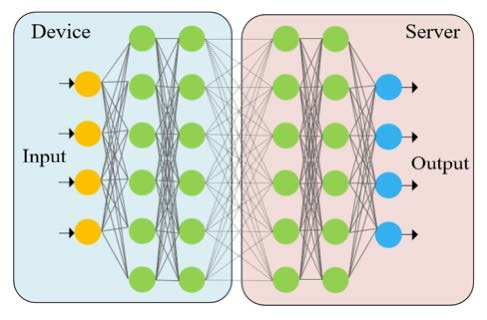
\includegraphics[width=0.75\textwidth]{./figure/0.jpg}  
    \caption*{图1.分割学习的服务器端与客户端的模型分布示例}
\end{figure}

在多本地终端与边缘服务器的情形下,我们有两种⽅案,⼀种是共享本地权重模型,也就是本地终端进⾏部分前向传播,随后将
输出张量和标签传送到边缘服务器端,边缘服务器端进⾏剩余的前向传播与部分反向传播,随后将经过处理的张量传输到本地终端,
本地终端完成剩余的反向传播,随后边缘服务器端得到所有⽤户的完整的梯度信息后进⾏平均,完成对模型参数进⾏更新。另外⼀种
是不共享本地权重模型,即在本地终端只需要进⾏部分的前向传播算法,将计算得到的激活单元的值上传⾄边缘服务器端,服务器接
着进⾏剩余的前向传播与完整的反向传播算法,随后得到本地终端的梯度信息对该本地终端的模型参数进⾏更新。

需要注意的是模型分割机制只能适合层与层之间不耦合的DNN,对于RNN等模型不适⽤。对于监督学习,终端需要将对应的label
信息上传⾄服务器,但该步骤不会泄露数据隐私,数据的标签只是判断的结果。本地终端不需要完整的前向与反向传播算法,将⼤部
分的计算任务卸载⾄边缘服务器端执⾏,节省本地计算资源。另外,终端不需要上传完整的梯度信息,取⽽代之的是部分激活单元的
值,在⼀定程度上减少了数据传输量。

\section{系统模型}
\subsection{模型参数}
⾸先我们假设分割点为$k$,整个神经⽹络的层数为$n$, $Batch\_Size$为每次模型迭代时处理数据量的⼤⼩。

假设进⾏训练的⽹络数据权重为$W=\{w_1,w_2,\dots,w_n\}$ ,其中$w_k$表示的是第$k$层时的模型参数数据量。

随后假设每层的输出的数据量记为$T=\{t_1,t_2,\dots,t_n\}\times Batch\_Size$,其中$t_k$表示的是第$k$层时的输出数据量。

正向传播的计算量$C_f = \{ c_{f1},c_{f2},\dots,c_{fn} \}\times Batch\_Size$,其中$c_{fk}$表示的是第$k$层的正向传播的计算量。

反向传播的计算量$C_f = \{c_{b1},c_{b2},\dots,c_{bn}\}\times Batch\_Size$,其中$c_{fk}$表示的是第$k$层的反向传播的计算量。

\subsection{模型结构}
\subsubsection{共享本地权重模型}
本地终端进⾏部分前向传播,随后将输出张量和标签传送到边缘服务器端,边缘服务器端进⾏剩余的前向传播与部分反向传播,
随后将经过处理的张量传输到本地终端,本地终端完成剩余的反向传播,随后边缘服务器端得到所有⽤户的完整的梯度信息后进⾏平
均,完成对模型参数进⾏更新。这样的⼀个流程完成⼀次迭代,这个过程⼀直持续到收敛。具体细节如图2所示。


\begin{figure}[H]
    \centering
    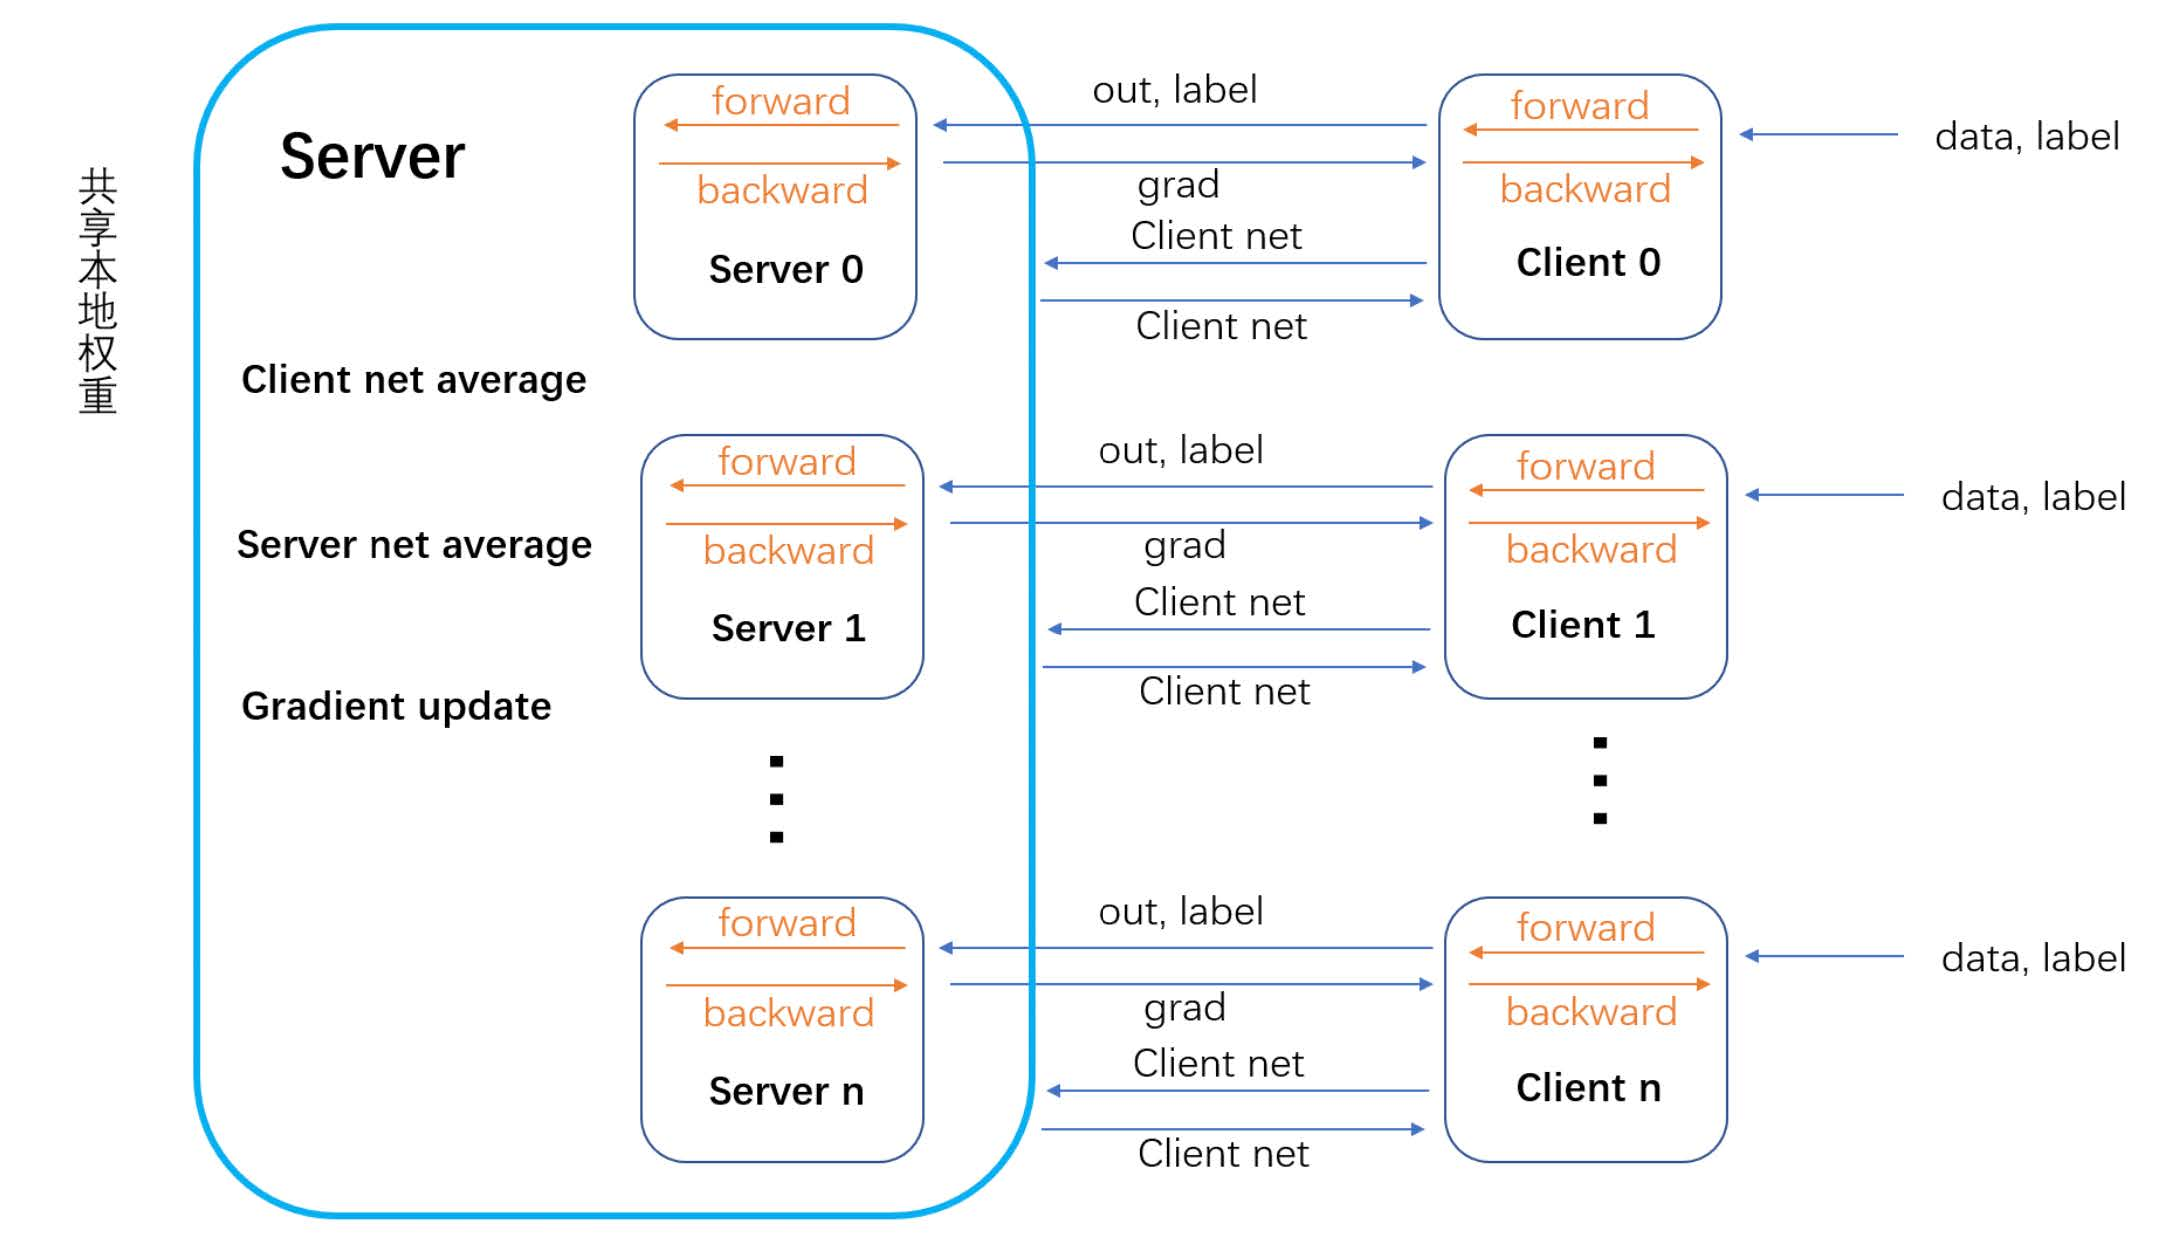
\includegraphics[width=0.85\textwidth]{./figure/1.jpg}  
    \caption*{图2.共享本地权重模型}
\end{figure}


\subsubsection{不共享本地权重模型}
本地终端只需要进⾏部分的前向传播算法,将计算得到的激活单元的值上传⾄边缘服务器端,服务器接着进⾏剩余的前向传播与
完整的反向传播算法,随后得到本地终端的梯度信息,对该本地终端的模型参数进⾏更新。这样的⼀个流程完成⼀次迭代,这个过程
⼀直持续到收敛。具体细节如图3所示。

\begin{figure}[H]
    \centering
    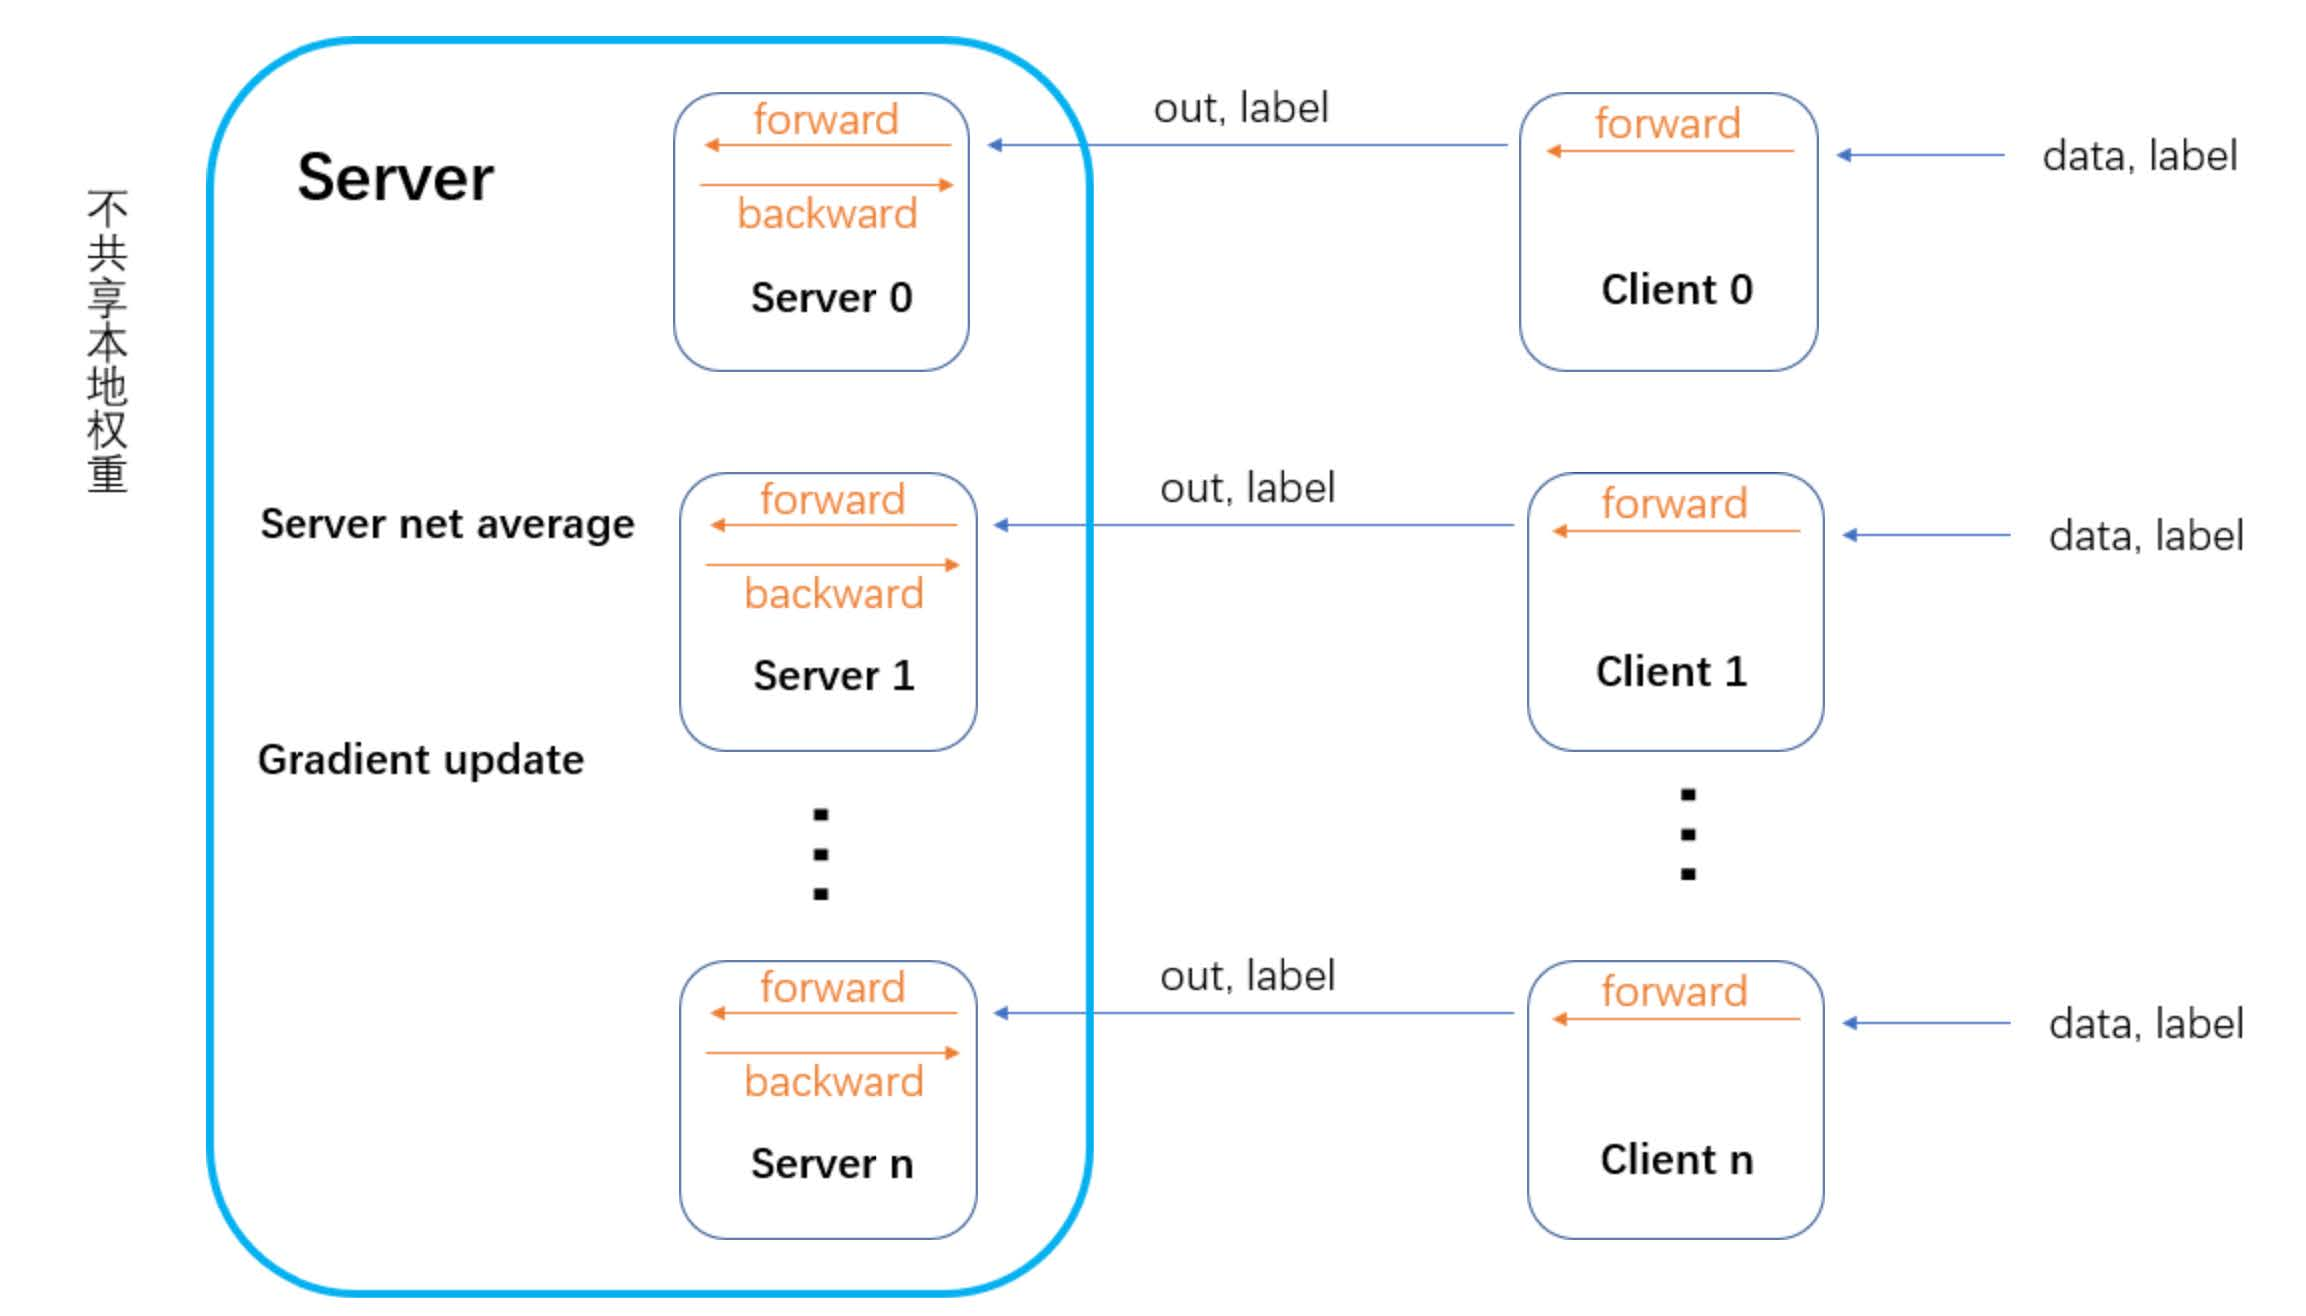
\includegraphics[width=0.85\textwidth]{./figure/2.jpg}  
    \caption*{图3.不共享本地权重模型}
\end{figure}

\subsubsection{传统联邦学习模型}
在本地终端完成完整的前向传播和反向传播,将权重更新参数传到边缘服务器,边缘服务器对其进⾏平均与更新权重,随后更新后的
权重传回本地终端。这样的⼀个流程完成⼀次迭代,这个过程⼀直持续到收敛。具体细节如图4所示。

\begin{figure}[H]
    \centering
    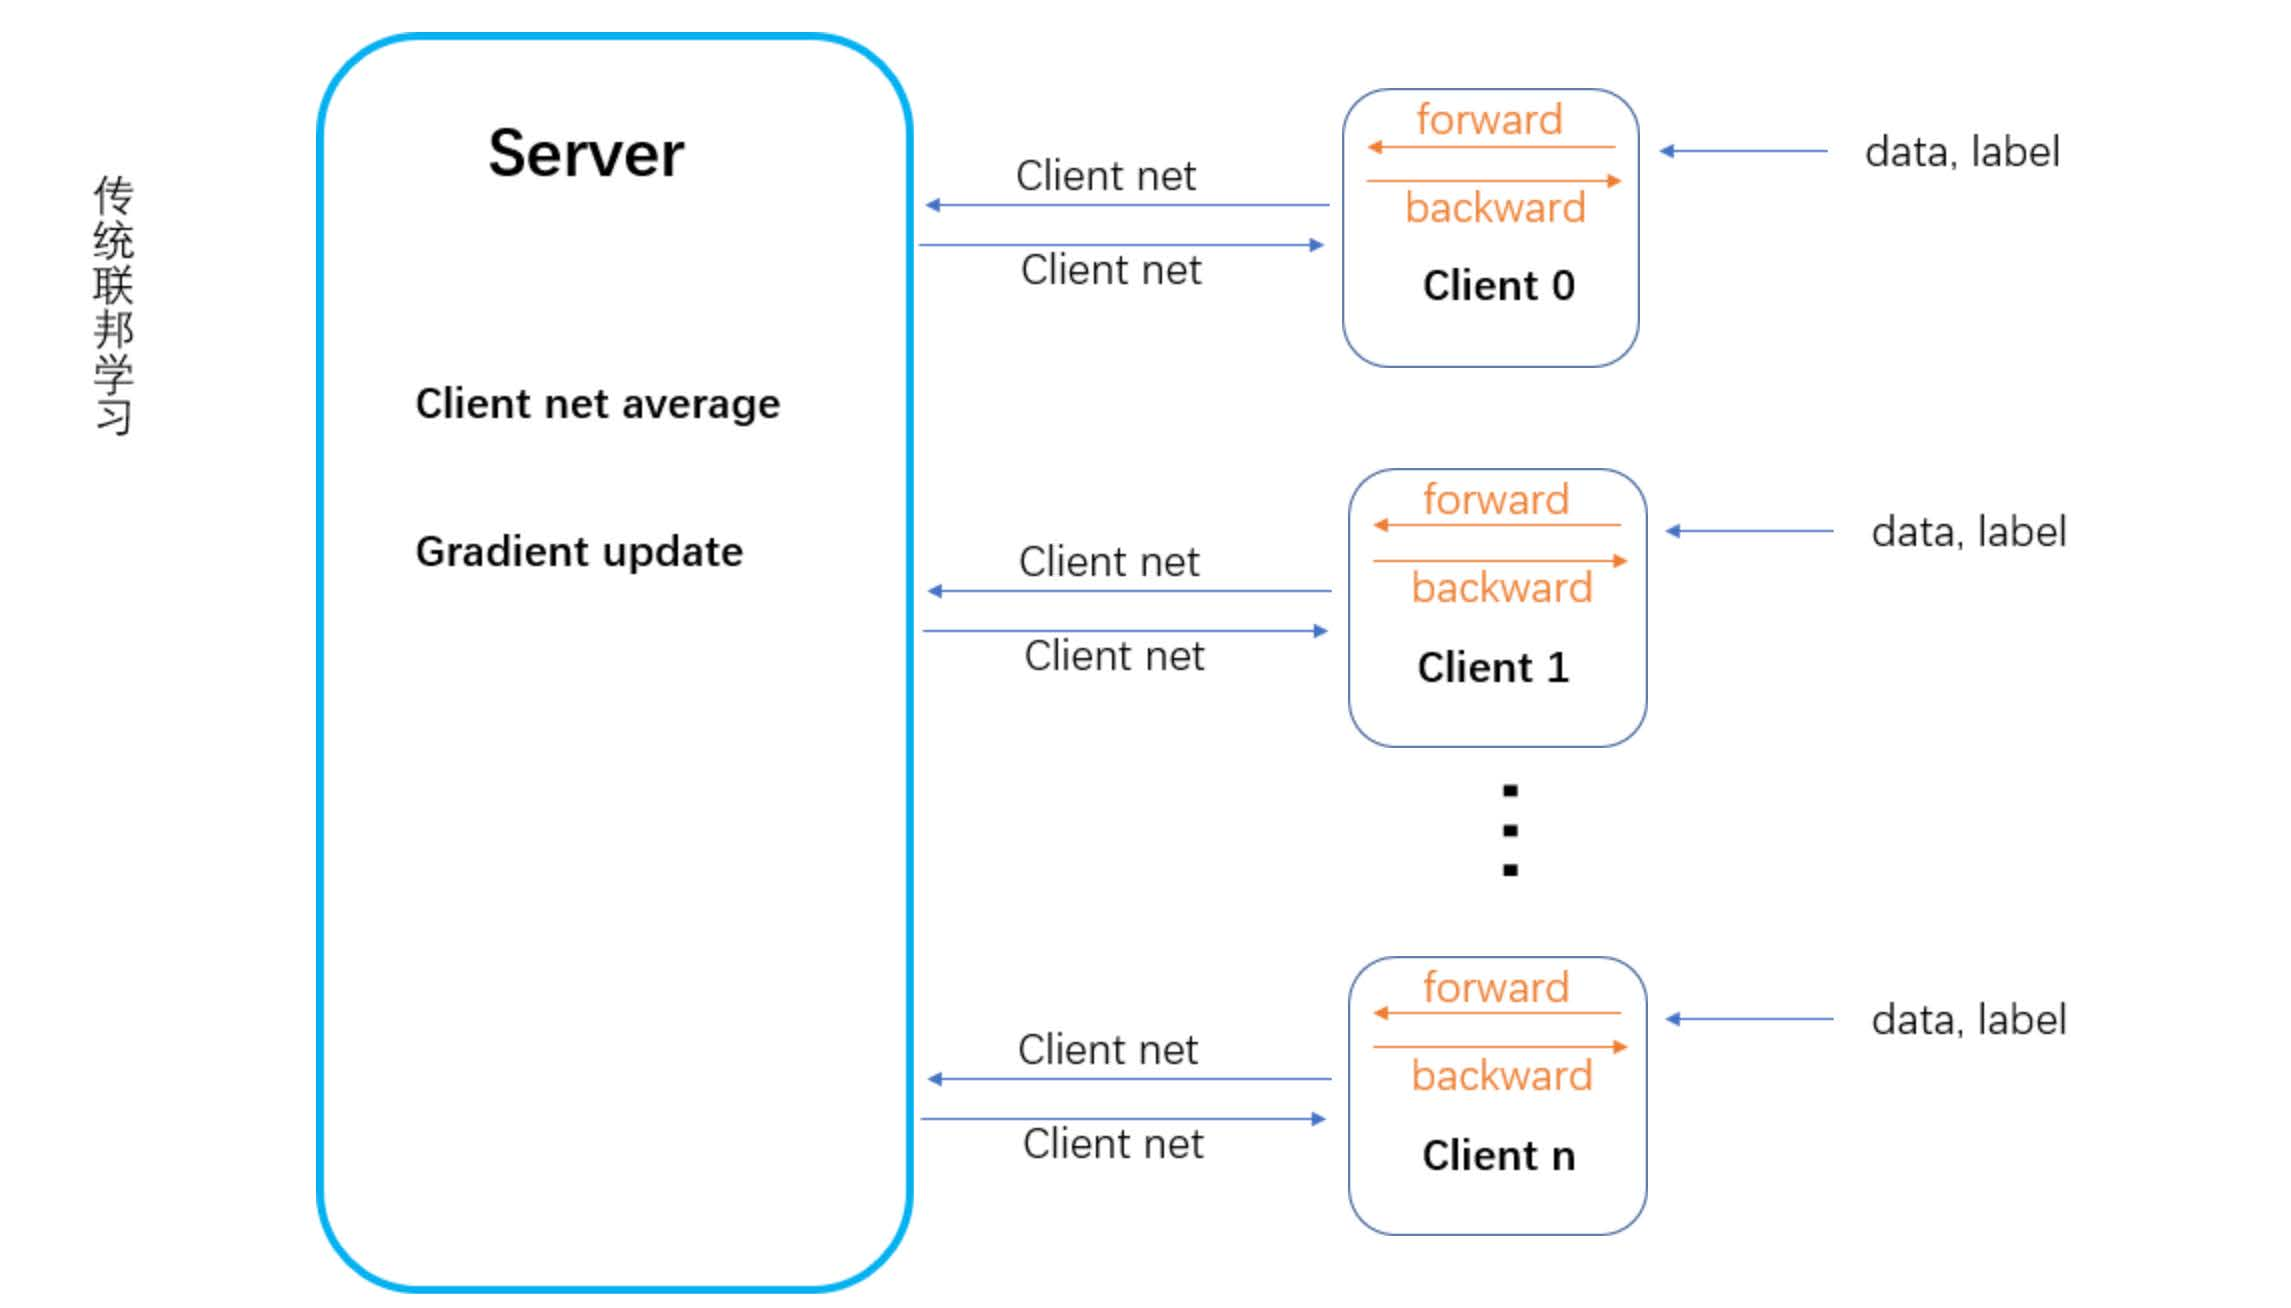
\includegraphics[width=0.85\textwidth]{./figure/3.jpg}  
    \caption*{图4.传统联邦学习模型}
\end{figure}

\section{模型分析与优化}

\subsection{参数分析}
我们对以上两种分割学习的模型进⾏了计算量的分析并且与传统联邦学习进⾏了⽐较。
\subsubsection{共享本地权重模型}
对于单个⽤户⽽⾔,当分割点为时的客户端前向传播的计算数据量$C_{forword}(k)$可以计算为每次传输数据量$(Batch\_Size)$与之前层前向传播的数据量和的乘积。
\begin{equation}
    \centering
    C_{forward}(k)=Batch\_Size\times \sum_{i=1}^k c_{fi}
\end{equation}

当分割点为时的客户端反向传播的计算数据量$C_{backword}(k)$可以计算为每次传输数据量$(Batch\_Size)$与之前层反向传播的数据量和的乘积。
\begin{equation}
    \centering
    C_{backward}(k)=Batch\_Size\times \sum_{i=1}^k c_{bi}
\end{equation}

因此我们可以得到当分割点为时的客户端的本地总体计算量$C_{client}(k)$为当分割点为$k$时的客户端前向传播的计算数据量与当分割点
为$k$时的客户端反向传播的计算数据量之和。
\begin{align}
    C_{client}(k) & =C_{forward}(k)+C_{backward}(k) \notag\\
    & =Batch\_Size\times (\sum_{i=1}^k c_{fi}+\sum_{i=1}^k c_{bi})
\end{align}

设单个⽤户到服务器端的总传输量为$T_{all}(k)$,其中训练数据传输量为$T_{data}(k)$,标签传输量为$T_{label}(k)$,梯度回传数据量为$T_{grad}(k)$,网络权重梯度传输量为$T_{net}(k)$,因此有:
\begin{equation}
    \centering
    T_{data}(k)=Batch\_Size\times t_k
\end{equation}

\begin{equation}
    \centering
    T_{label}(k) = Batch\_Size
\end{equation}

\begin{equation}
    \centering
    T_{grad}(k) = Batch\_Size \times t_k
\end{equation}

\begin{equation}
    \centering
    T_{net}(k)=2\sum_{i=1}^k w_i
\end{equation}

所以,
\begin{align}
    T_{all}(k) & = T_{data}(k)+T_{label}(k)+ T_{grad}(k)+T_{net}(k) \notag\\
    & = Batch\_Size \times (2t_k+1)+2\sum_{i=1}^k w_i
\end{align}

\subsubsection{不共享本地权重模型}
对于单个⽤户⽽⾔,当分割点为$k$时的客户端的本地总体计算量$C_{client}(k)$等于客户端前向传播的计算数据量$C_{forward}(k)$,即,
\begin{equation}
    C_{client}(k) = C_{forward}(k)=Batch\_Size\times \sum_{i=1}^k c_{fi}
\end{equation}

对于传输量,
\begin{equation}
    T_{data}(k)=Batch\_Size\times t_k
\end{equation}

\begin{equation}
    T_{label}(k) = Batch\_Size
\end{equation}

因此单个⽤户到服务器端的传输量为,
\begin{align}
    T_{all}(k) & = T_{data}(k)+T_{label}(k) \notag\\
    & = Batch\_Size \times (t_k+1)
\end{align}

\subsubsection{传统联邦学习}
对于单个⽤户⽽⾔,本地总体计算量$C_{client}$为客户端全部模型前向传播的计算数据量与客户端反向传播的计算数据量之和,即,
\begin{equation}
    \centering
    C_{forward}=Batch\_Size\times \sum_{i=1}^n c_{fi}
\end{equation}

\begin{equation}
    \centering
    C_{backward}=Batch\_Size\times \sum_{i=1}^n c_{bi}
\end{equation}

\begin{align}
    C_{client} & =C_{forward}+C_{backward} \notag\\
    & = Batch\_Size \times (\sum_{i=1}^n c_{fi}+\sum_{i=1}^n c_{bi})
\end{align}


对于传输量,传统联邦学习只传输了网络模型梯度数据,因此传输总量等于传输整个模型梯度数据,即,
\begin{equation}
    T_{all}(k)=T_{net}=2\sum_{i=1}^n w_i    
\end{equation}

\subsubsection{三种模型分析结论}

\begin{table}[H]
    \caption*{表1.三种模型方式的不同开销对比}
    \centering
    \begin{tabular}{lll}
    \toprule
    模型方法 & 单⽤户计算开销单 & 单⽤户传输开销\\
    \midrule
    共享本地权重(分割点为$k$) & $Batch\_Size(\sum_{i=1}^k c_{fi}+\sum_{i=1}^k c_{bi})$ & $Batch\_Size(2t_k+1)+2\sum_{i=1}^k w_i$\\
    不共享本地权重(分割点为$k$) & $Batch\_Size \sum_{i=1}^k c_{fi}$ & $Batch\_Size (t_k+1)$\\
    传统联邦学习 & $Batch\_Size (\sum_{i=1}^n c_{fi}+\sum_{i=1}^n c_{bi})$ & $2\sum_{i=1}^n w_i$\\
    \bottomrule
    \end{tabular}
\end{table}

\subsection{分割点优化}

模型卸载量影响着本地计算的时延以及数据上传的时延,终端卸载的模型规模越⼤,本地计算的时延越⼩,但此时增加了边缘服
务器的计算任务。反之,当终端的卸载模型规模越⼩,本地要承担计算量变多。计算量和通信传输量来的⼤⼩也可以直观的反映传输
的开销,因此我们可以使⽤传输所需的数据量的⼤⼩来估计传输的效率。我们可以设⽴⼀个评估函数来表示训练开销,训练开销是本
地计算量和数据传输量两部分的加权和,可以表示为,
\begin{equation}
    V=\alpha C+\beta T 
\end{equation}

其中$C$是本地计算量,$T$为传输量,$\alpha,\beta$为系数权重,根据本地计算能力和和服务器通信能力确定,⽤于平衡本地计算量和传输量的⼤⼩。

因此在共享本地权重的模型中,我们可以计算出其单步总开销为,
\begin{equation}
    V=\alpha \times Batch\_Size \times (\sum_{i=1}^k c_{fi}+\sum_{i=1}^k c_{bi})+\beta \times (Batch\_Size \times (2t_k+1)+2\sum_{i=1}^k w_i)
\end{equation}

同理,在不共享本地权重的模型中,我们可以计算出其单步总开销为,
\begin{equation}
    V=\alpha \times Batch\_Size \times \sum_{i=1}^k c_{fi}+\beta \times Batch\_Size \times (t_k+1)
\end{equation}


⽽传统的联邦学习模型中,我们可以得到单步总开销为,
\begin{equation}
    V=\alpha \times Batch\_Size \times (\sum_{i=1}^n c_{fi}+\sum_{i=1}^n c_{bi})+\beta \times 2\sum_{i=1}^n w_i
\end{equation}

可以从中看出不共享本地权重的模型分割⽅法,虽然牺牲了⼀点模型训练性能,但可以进⼀步减少数据传输量以及本地运算量。此外我们需要最
⼩化这个学习开销,得到最优的分割点,得到最优的分割⽅案。

\section{仿真设计}
\subsection{深度学习模型设计}
我们采⽤的神经⽹络模型是$LeNet$,数据集采⽤的是$MNIST$⼿写数字识别数据集。其中我们的$LeNet$模型具体参数如图5所示,其中前6层是两遍的卷积和池化,然后展平数据后,最后通过三层全连接神经网络。

本文设置测试点为每迭代一次,测试一次测试集损失和准确率,训练$Batch\_Size$设置为$500$大小,用户个数为$10$,迭代$800$个批次。并设置好随机种子不变以保证每次迭代运算相同。
\begin{figure}[H]
    \centering
    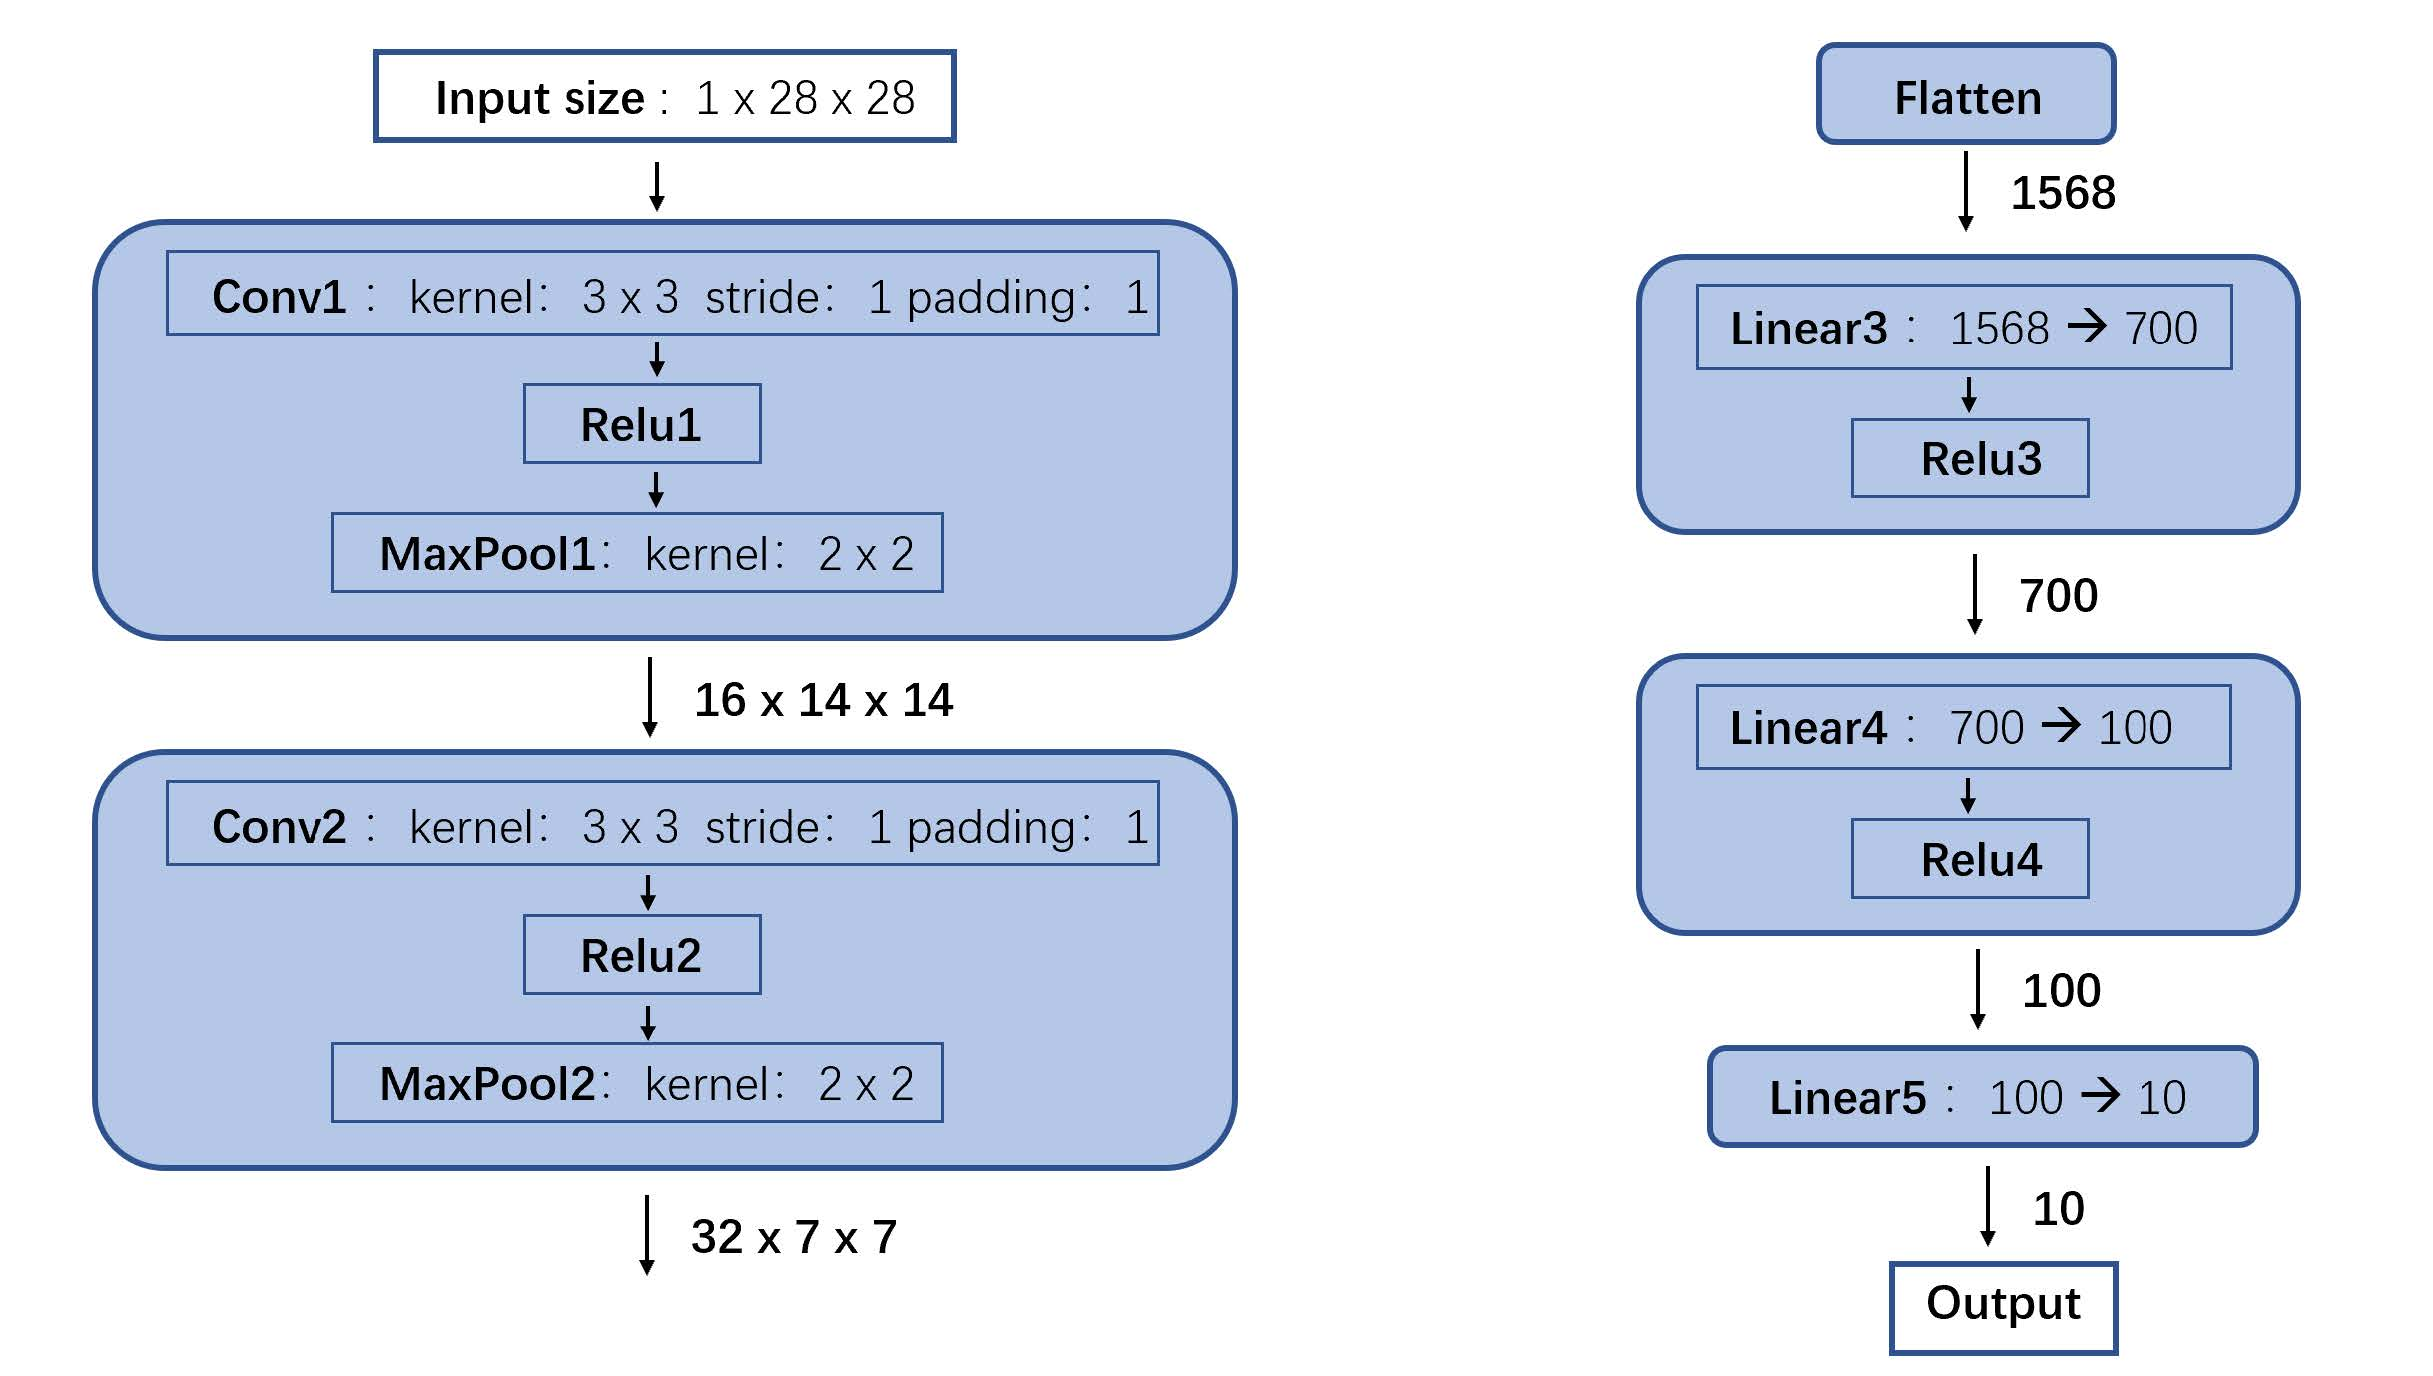
\includegraphics[width=0.85\textwidth]{./figure/4.jpg}  
    \caption*{图5.深度学习网络仿真模型}
\end{figure}

其中每⼀层的⽹络数据权重$W$,输出数据量$T$,每层正向传播的计算量$C_{forward}$,反向传播的计算量$C_{backward}$,如下表所示,

\begin{table}[H]
    \caption*{表2.仿真学习模型的计算量和传输量}
    \centering
    \begin{threeparttable}
    \begin{tabular}{lllll}
    \toprule
    Layer Name & $W$ & $T$ & $C_{forward}/Device$ & $C_{backward}/Device$\\
    \midrule
    Conv1 & 160 & 12544 & 250880 & 250880 \\
    Relu1 & 0 & 12544 & 0 & 0\\
    MaxPool1 & 0 & 3136 & 0 & 0\\
    Conv2 & 4640 & 6272 & 909440 & 909440\\
    Relu2 & 0 & 6276 & 0 & 0\\
    MaxPool2 & 0 & 1568 & 0 & 0\\
    Flatten & 0 & 1568 & 0 & 0\\
    Linear3 & 1098300 & 700 & 1097600 & 1097600\\
    Relu3 & 0 & 700 & 0 & 0\\
    Linear4 & 70100 & 100 & 70000 & 70000\\
    Relu4 & 0 & 100 & 0 & 0\\
    Linear5 & 1010 & 10 & 1000 & 1000\\
    \bottomrule
    \end{tabular}
    \begin{tablenotes}[c]
        \footnotesize
        \item $W$: 需要传输的每层的网络数据权重。
        \item $T$: 网络分割点之后的截面数据量,需要从用户传输到主机的数据量。
        \item $C_{forward}/Device$: 在用户端正向传播的计算量,这里以浮点计算为主要考虑目标。
        \item $C_{backward}/Device$: 在用户端反向传播的计算量,本文认为其和正向传播计算量一致。
        \item 相对与卷积层和全连接层,池化层和激活函数运算量可以忽略。
    \end{tablenotes}
    \end{threeparttable}
    \end{table}
    
\subsection{仿真结果}
本文设置测试点为每迭代一次,测试一次测试集损失和准确率,训练$Batch\_Size$设置为$500$大小,用户个数为$10$,迭代$800$个批次。并设置好随机种子不变以保证每次迭代运算相同。

\subsubsection{迭代次数相关}
下图图6是随训练损失、测试集损失和准确率随迭代次数的关系。
\begin{figure}[H]
    \centering
    \subfigure[训练损失]{
        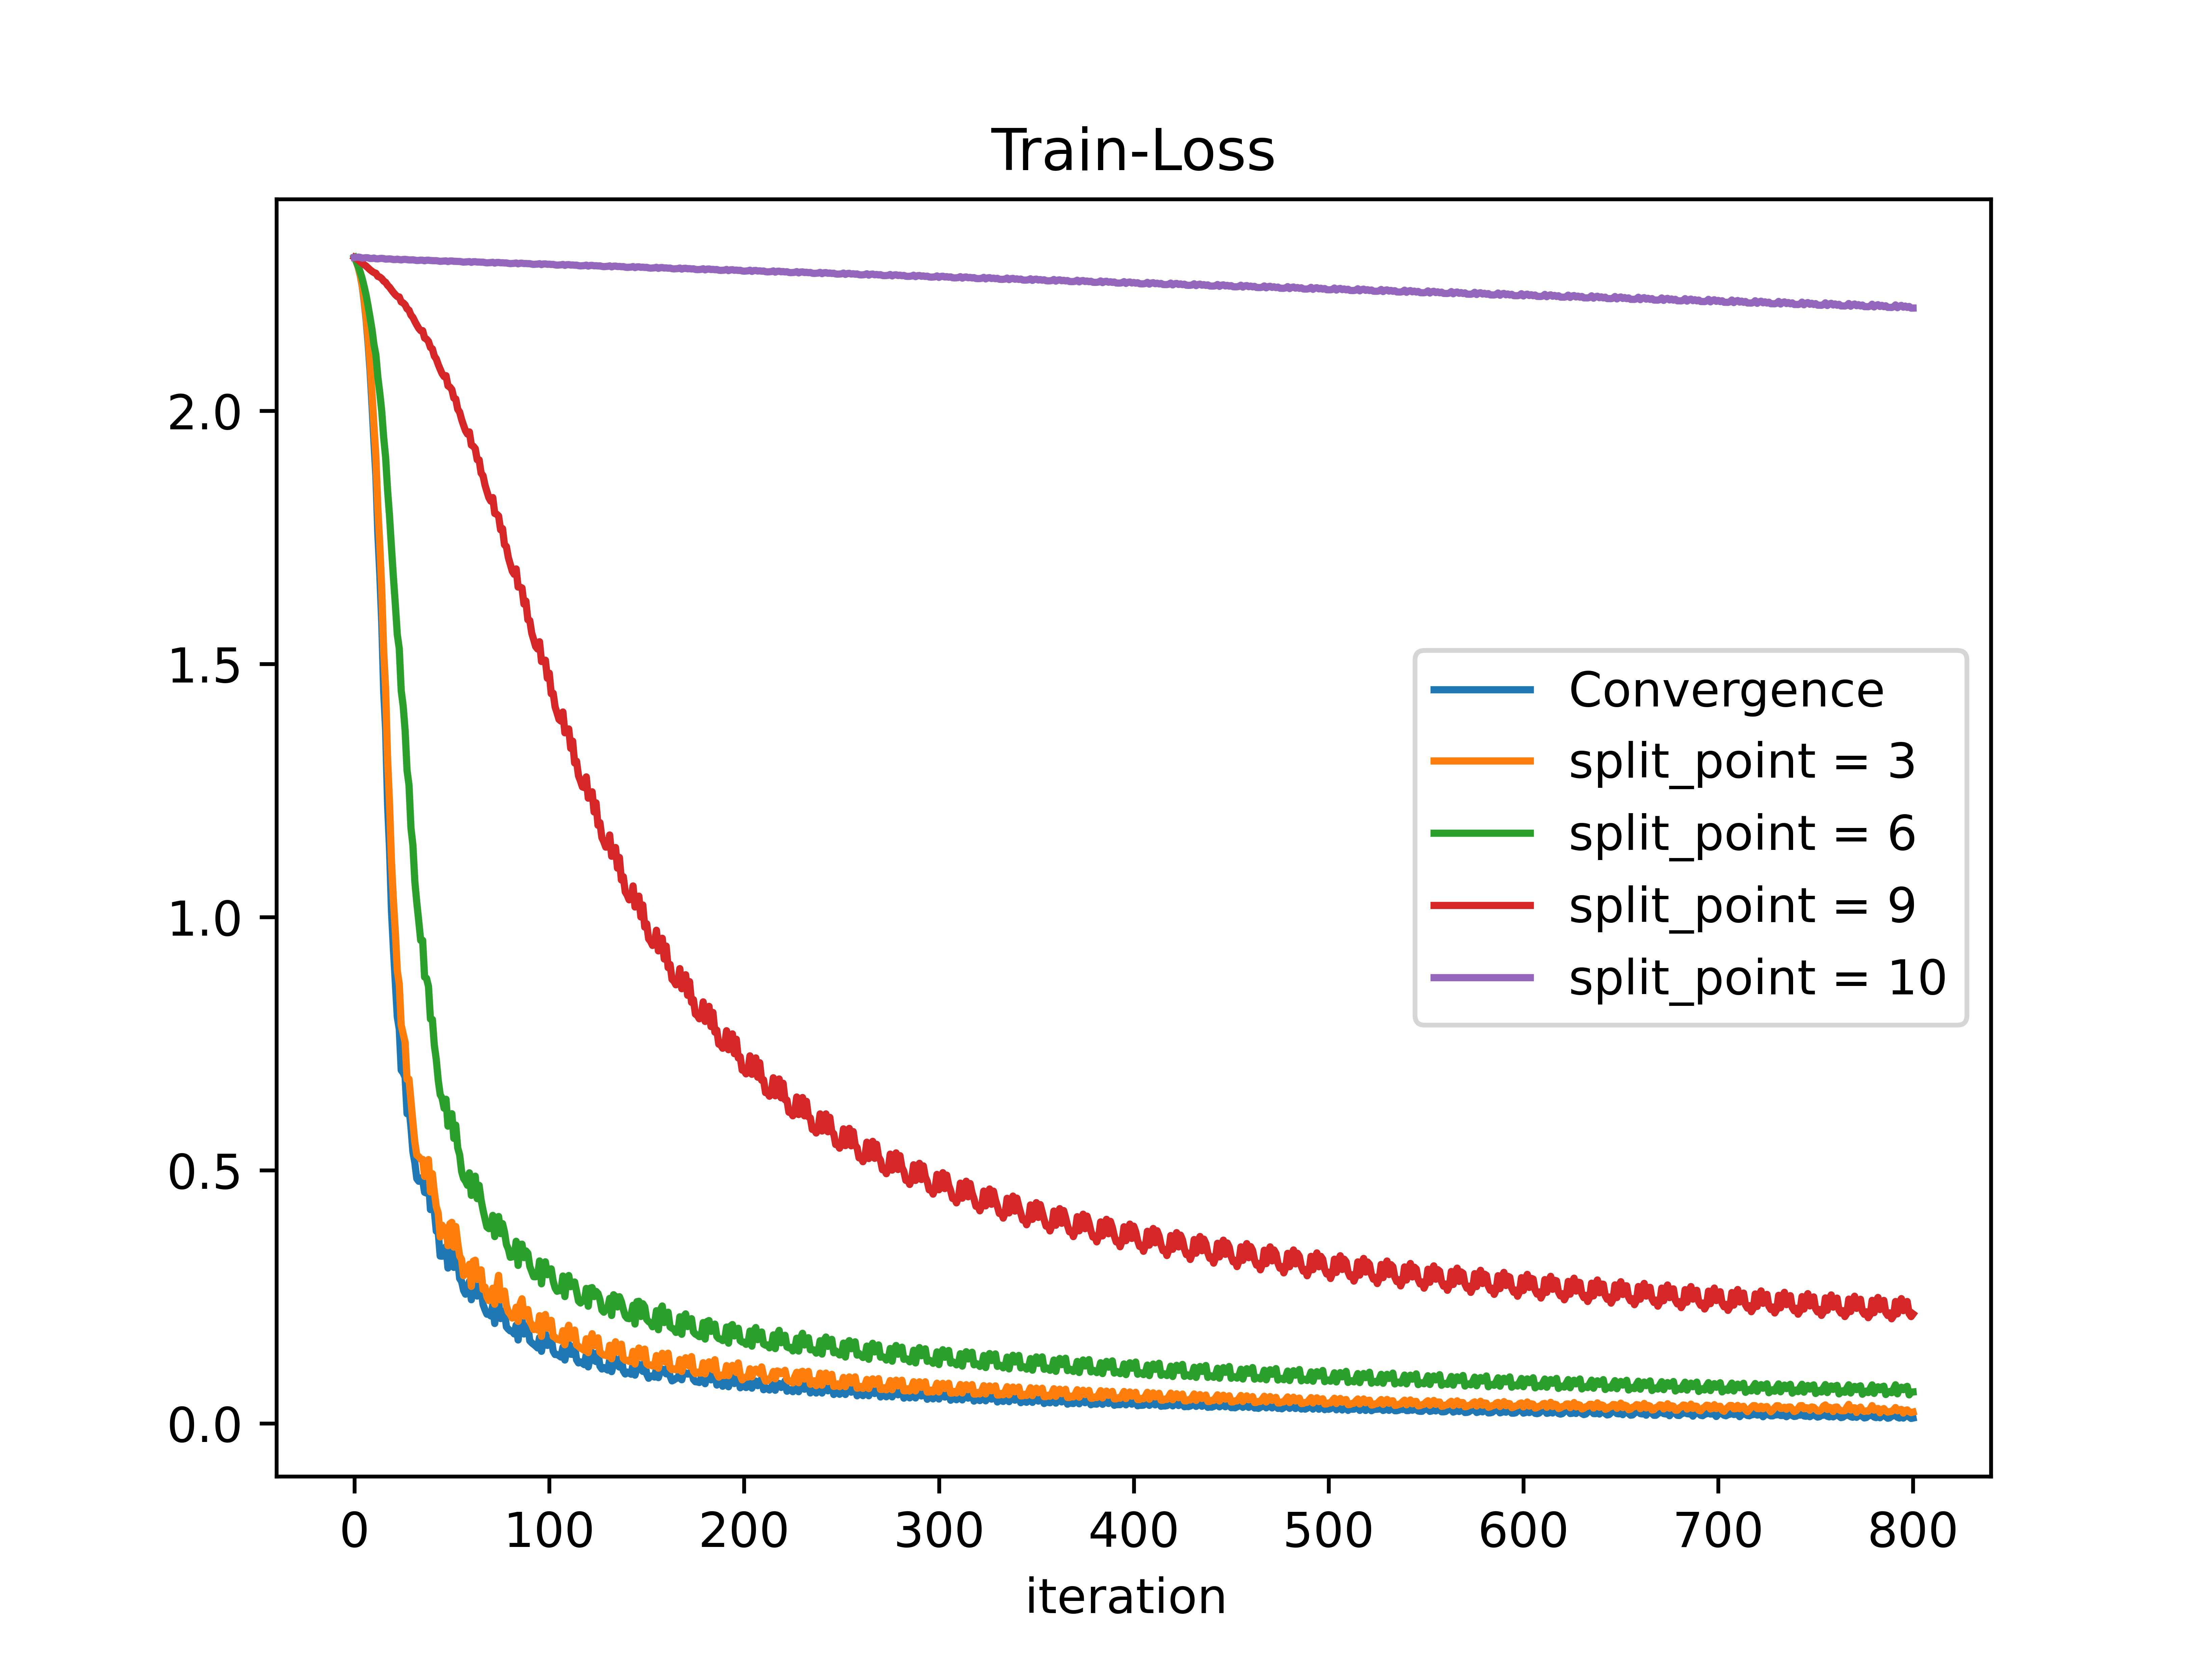
\includegraphics[width=0.45\textwidth]{pictures/Train_Loss.png}
    }
    \subfigure[测试集损失]{  
        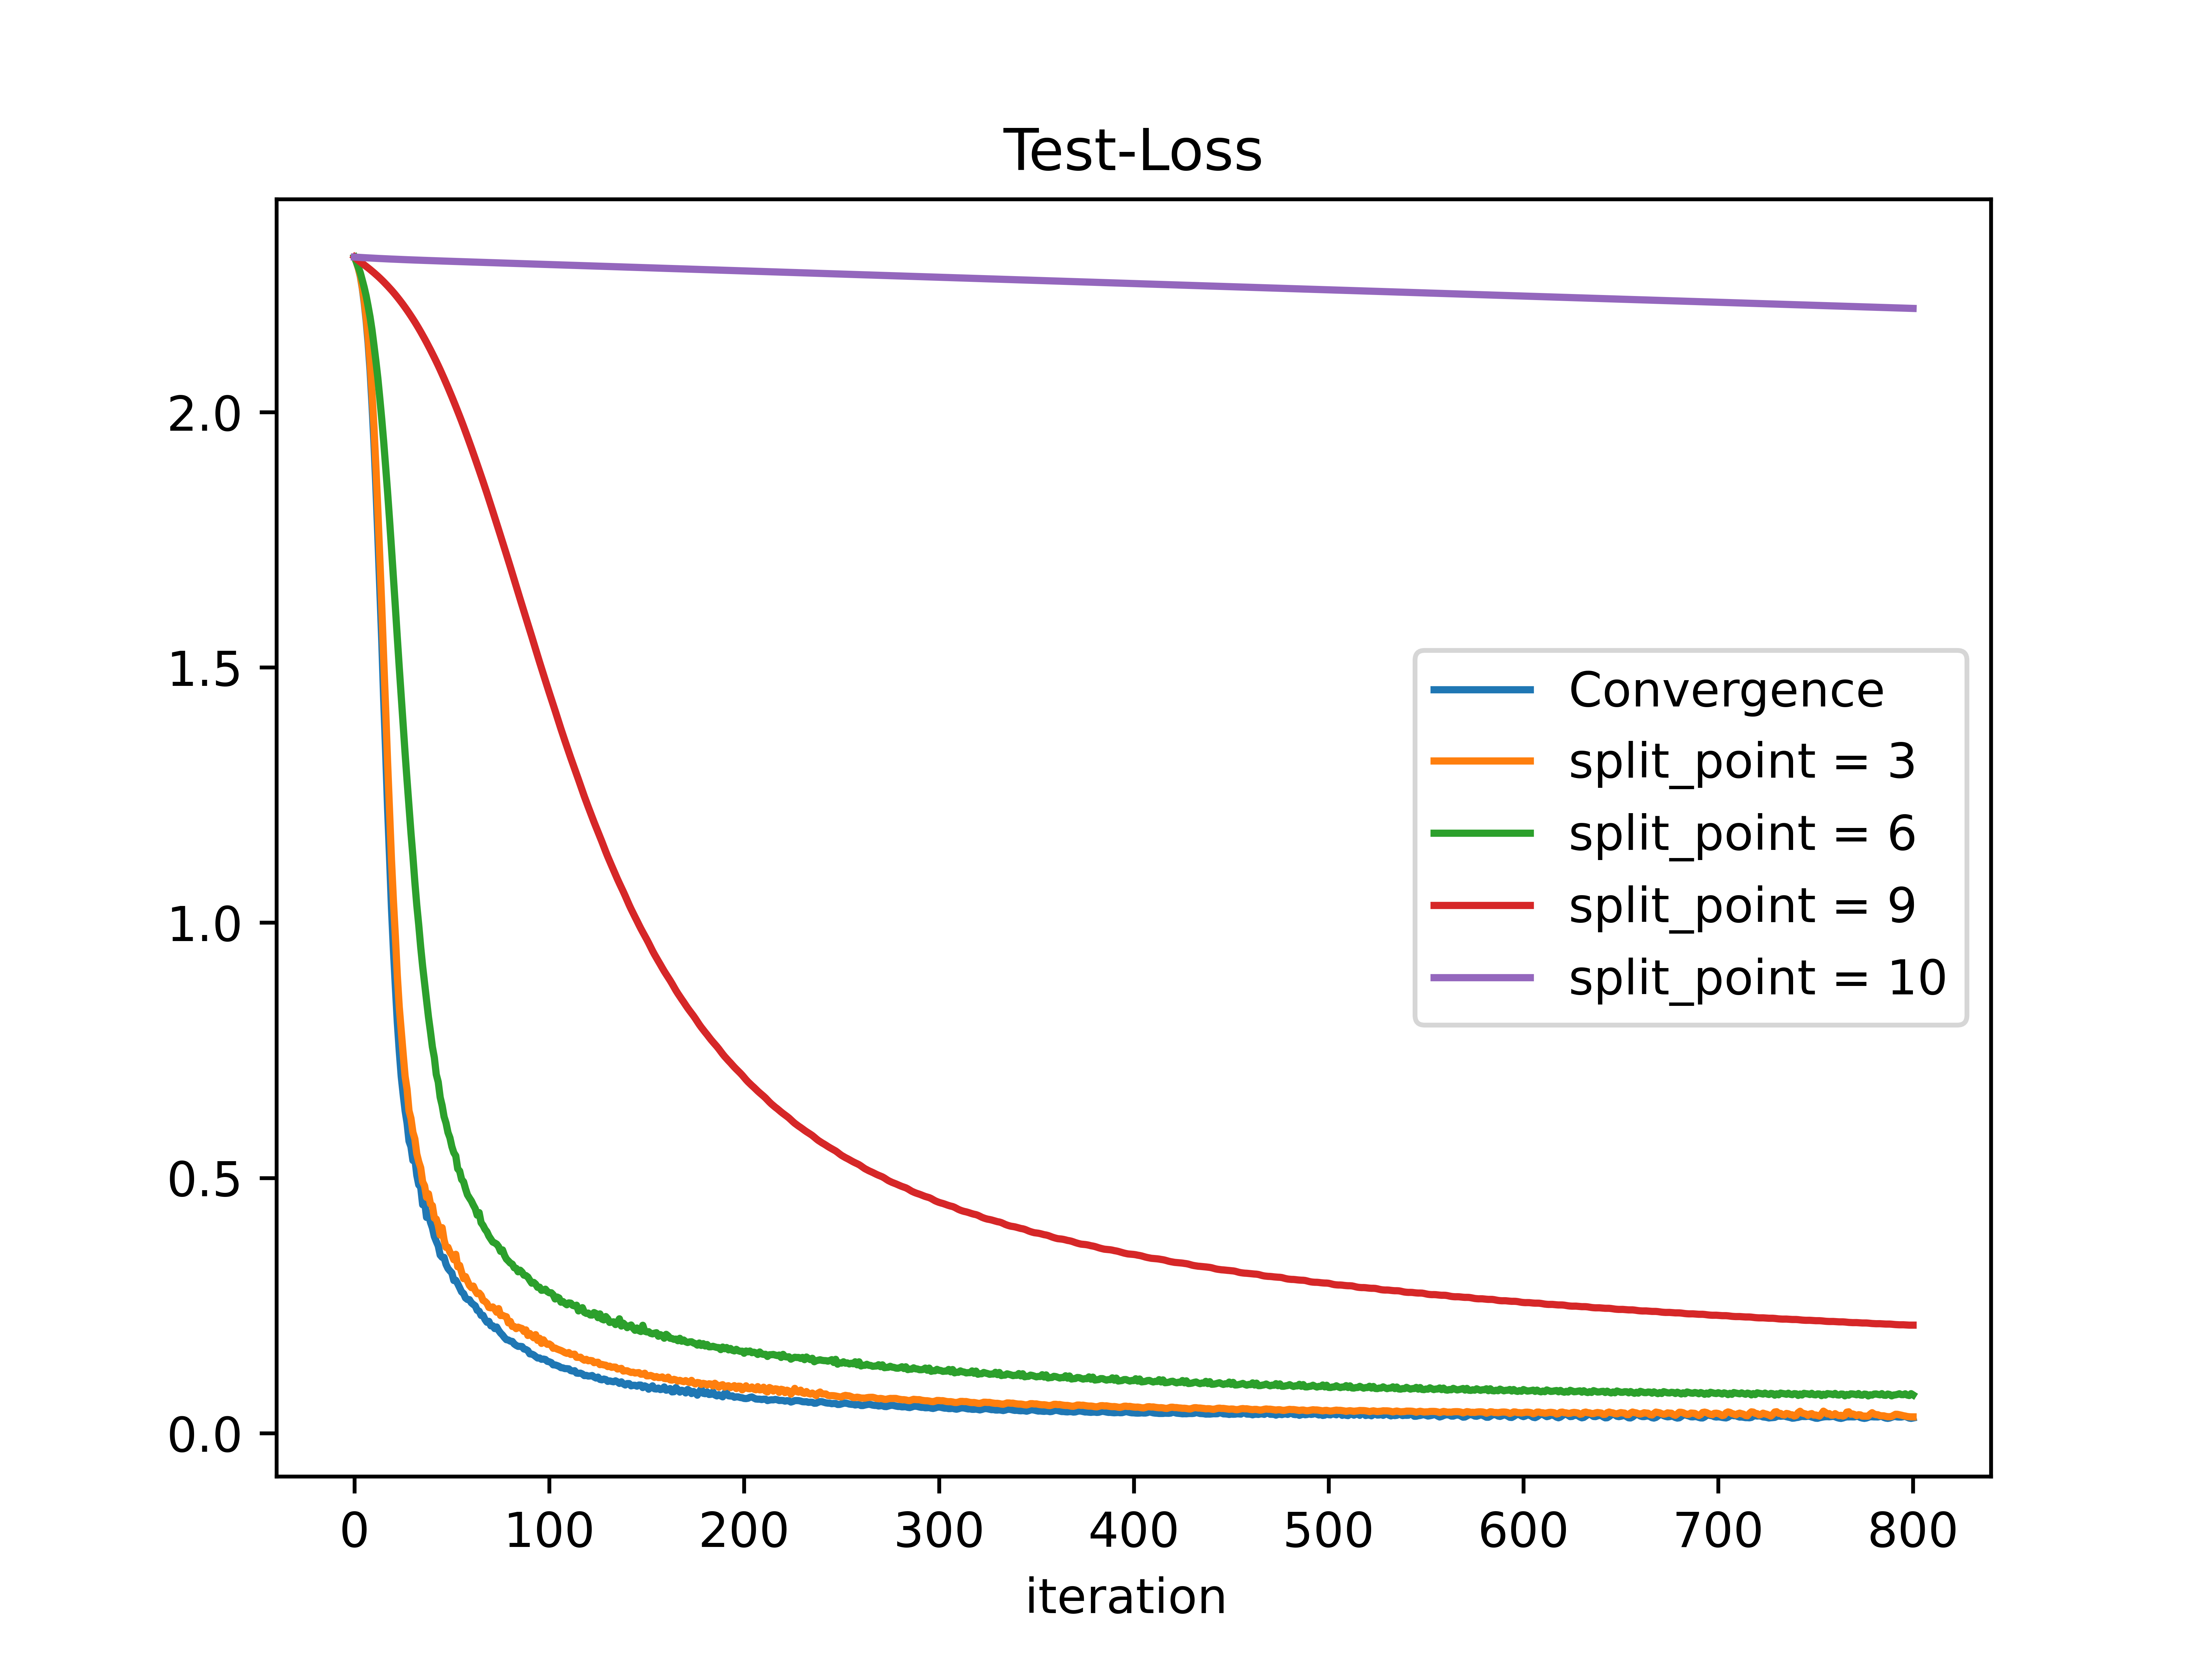
\includegraphics[width=0.45\textwidth]{pictures/Test_Loss.png}
    }
    \subfigure[测试集准确率]{
        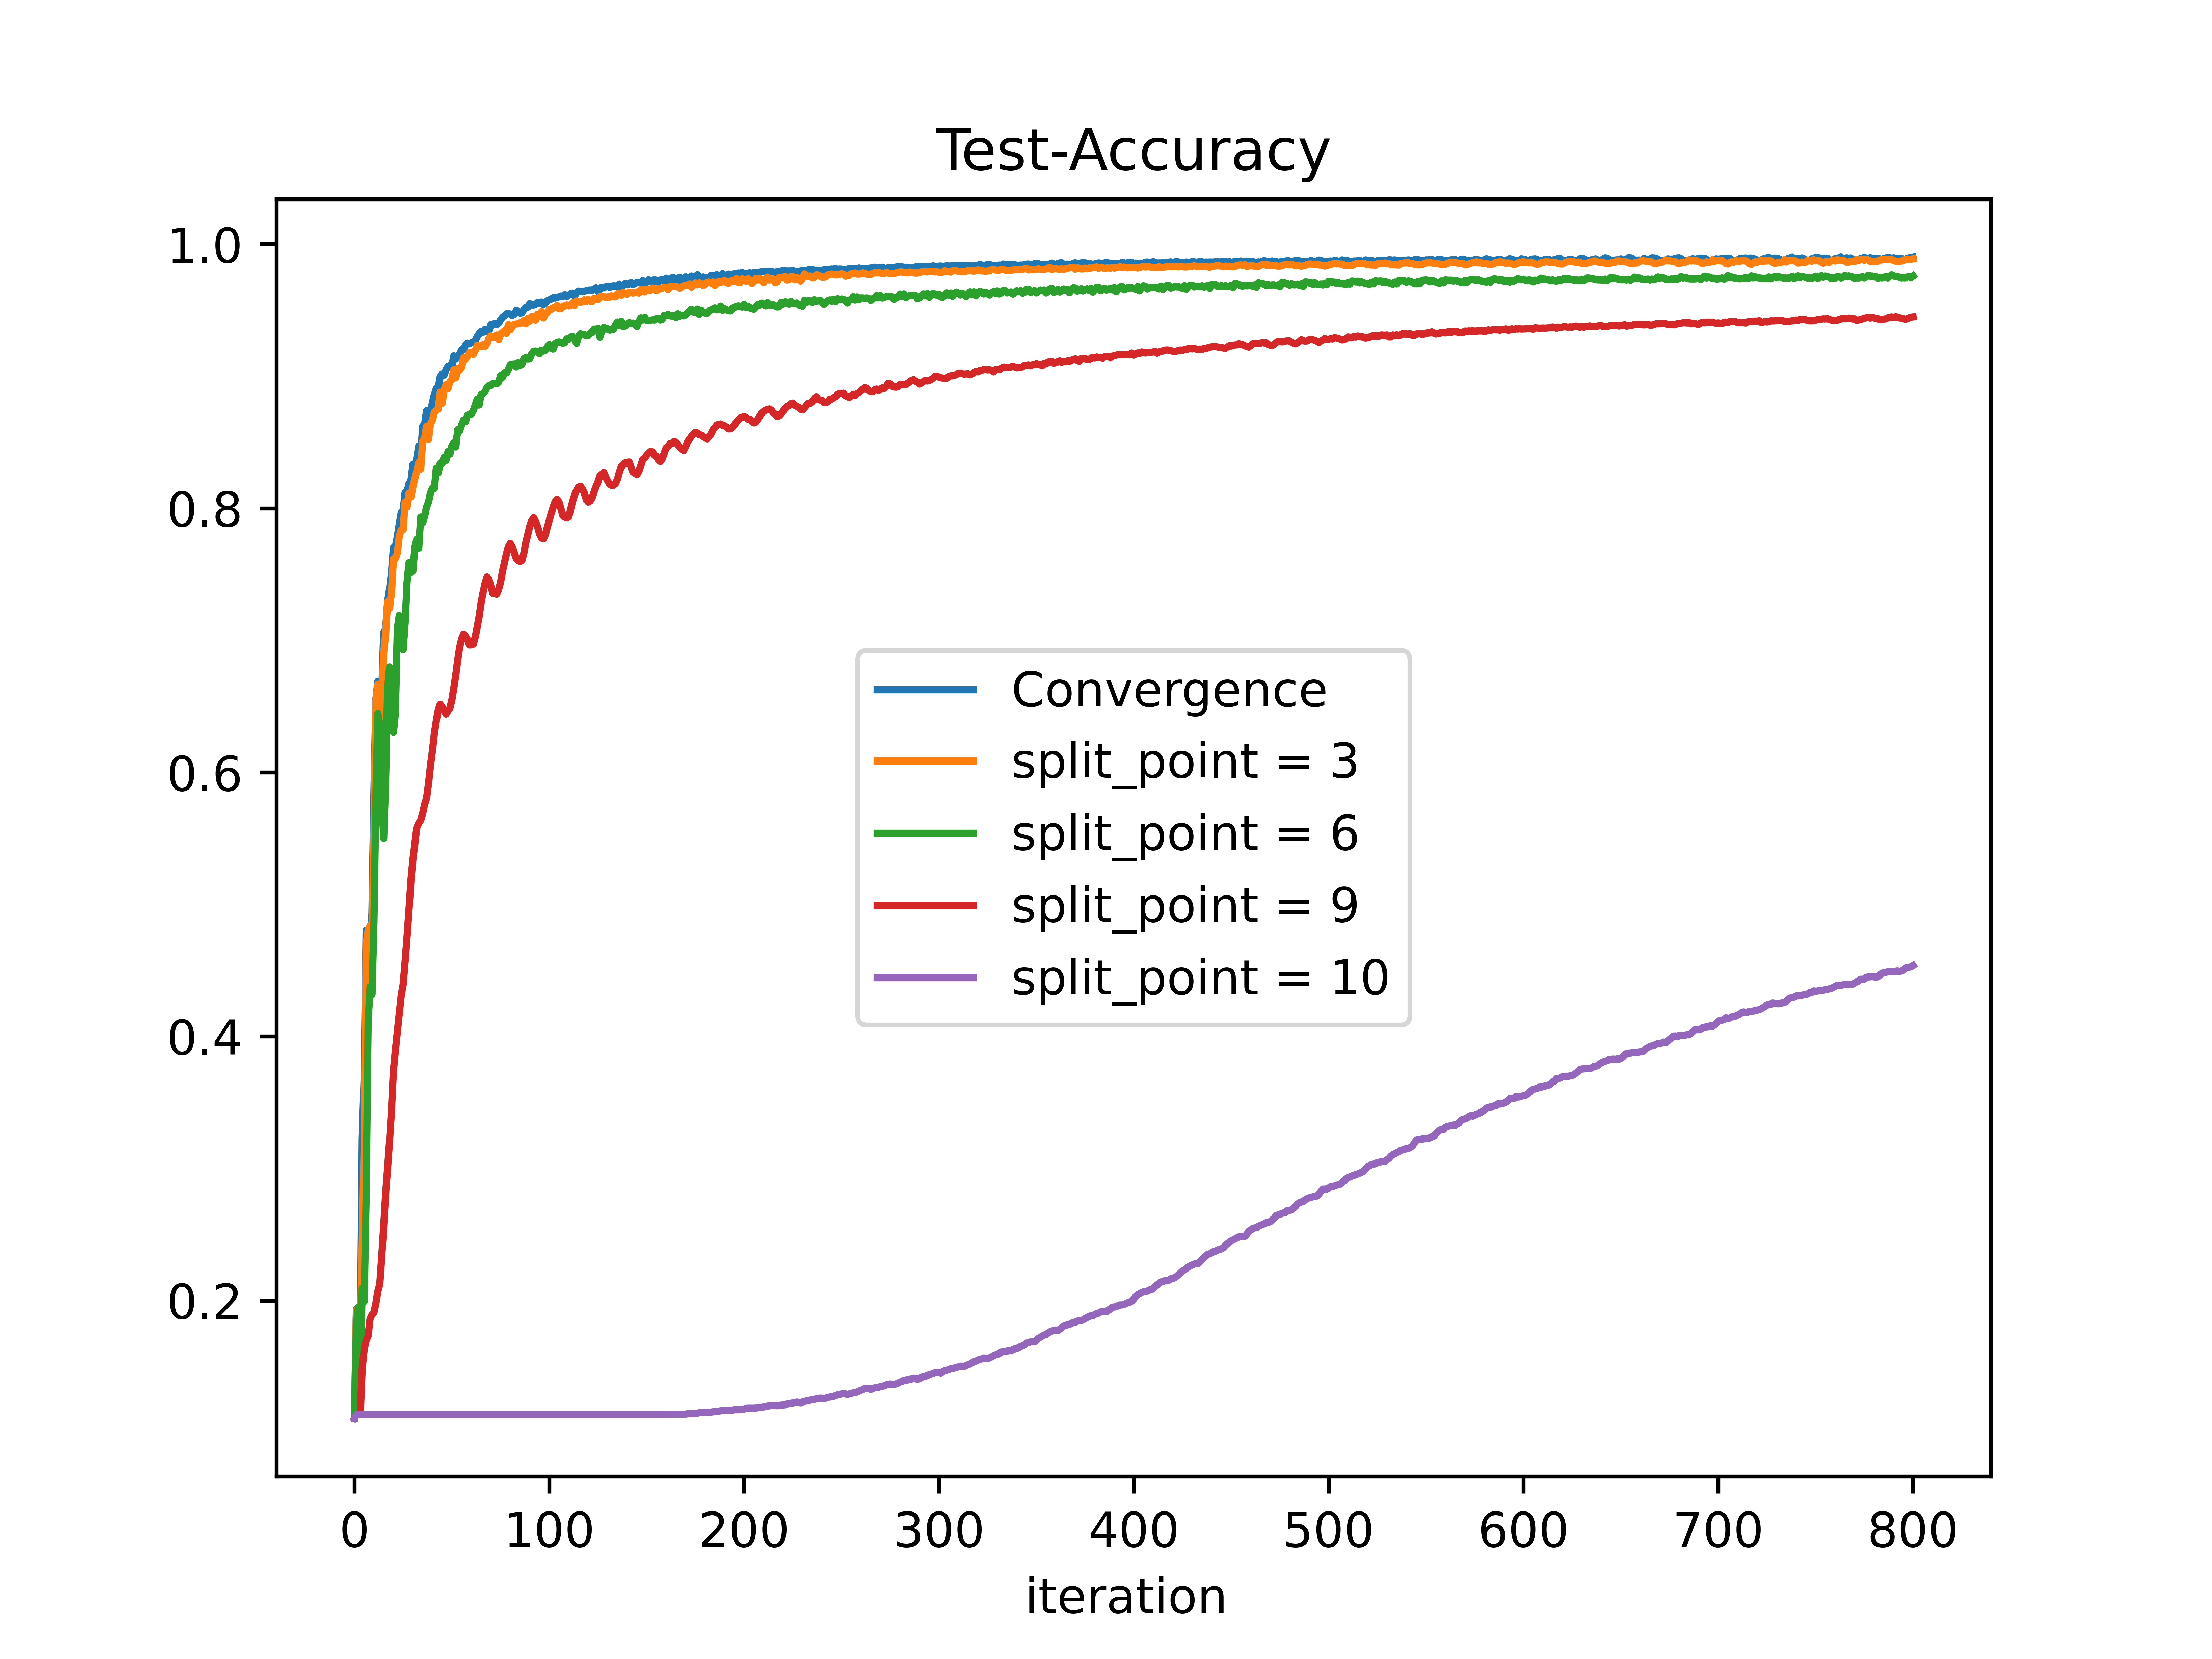
\includegraphics[width=0.45\textwidth]{pictures/Test_Accuracy.png}
    }
    \caption*{图6.共享本地权重模型与不共享本地权重模型的训练损失,测试损失,测试准确率}
\end{figure}

从图6可以看出,共享本地权重模型的不同分割点不影响训练损失,测试损失和测试准确率,并且其准确率最高,损失最小,并且收敛速率最快(相对于迭代次数来说),到最后准确率约为$97\%$。

⽽不共享本地权重模型⾥分割点$k$靠前可以得到更快的收敛速度(相对于迭代次数来说),并且对准确率和损失影响并不大。

\subsubsection{训练开销相关}
根据前文提到的训练开销$V=\alpha C +\beta T$,本文设置,
\begin{align}
    \alpha = 1\times 10^{-8} \notag \\
    \beta = 64 \times 10^{-6} 
\end{align}

因此可以得到三种模型方式以及不同分割点的不同训练开销,如下表3,

\begin{table}[H]
    \caption*{表3.三种方式以及不同分割点的训练开销}
    \centering
    \begin{threeparttable}
    \begin{tabular}{llll}
    \toprule
    分割层 & 共享本地权重 & 不共享本地权重 & 传统的联邦学习\\
    \midrule
    Conv1 & 82.79565 & 41.39840 & \multirow{12}{*}{20.99192}  \\
    Relu1 & 82.79565 & 41.39840 \\
    MaxPool1 & 22.58445 & 11.29280 \\
    Conv2 & 51.80864 & 25.87520\\
    Relu2 & 51.80864 & 25.87520 \\
    MaxPool2 & 21.70304 & 10.82240 \\
    Flatten & 21.70304 & 10.82240 \\
    Linear3 & 41.18208 & 13.53280 \\
    Relu3 & 41.18208 & 13.53280 \\
    Linear4 & 38.93936 & 11.96280\\
    Relu4 & 38.93936 & 11.96280 \\
    Linear5 & 38.38629 & 11.67980\\
    \bottomrule
    \end{tabular}
    \begin{tablenotes}[c]
        \footnotesize
        \item 这里设置$\alpha = 1\times 10^{-8} $, $\beta = 64 \times 10^{-6} $。
    \end{tablenotes}
    \end{threeparttable}
    \end{table}

根据表3,很明显,当$k=6$时共享本地权重的模型以及不共享本地权重的模型具有最小的训练开销。

\subsubsection{共享本地权重模型仿真}
根据表3的训练开销,我们可以得到共享本地权重相关的损失和准确率对于训练代价的图。
\begin{figure}[H]
    \centering
    \subfigure[训练损失]{
        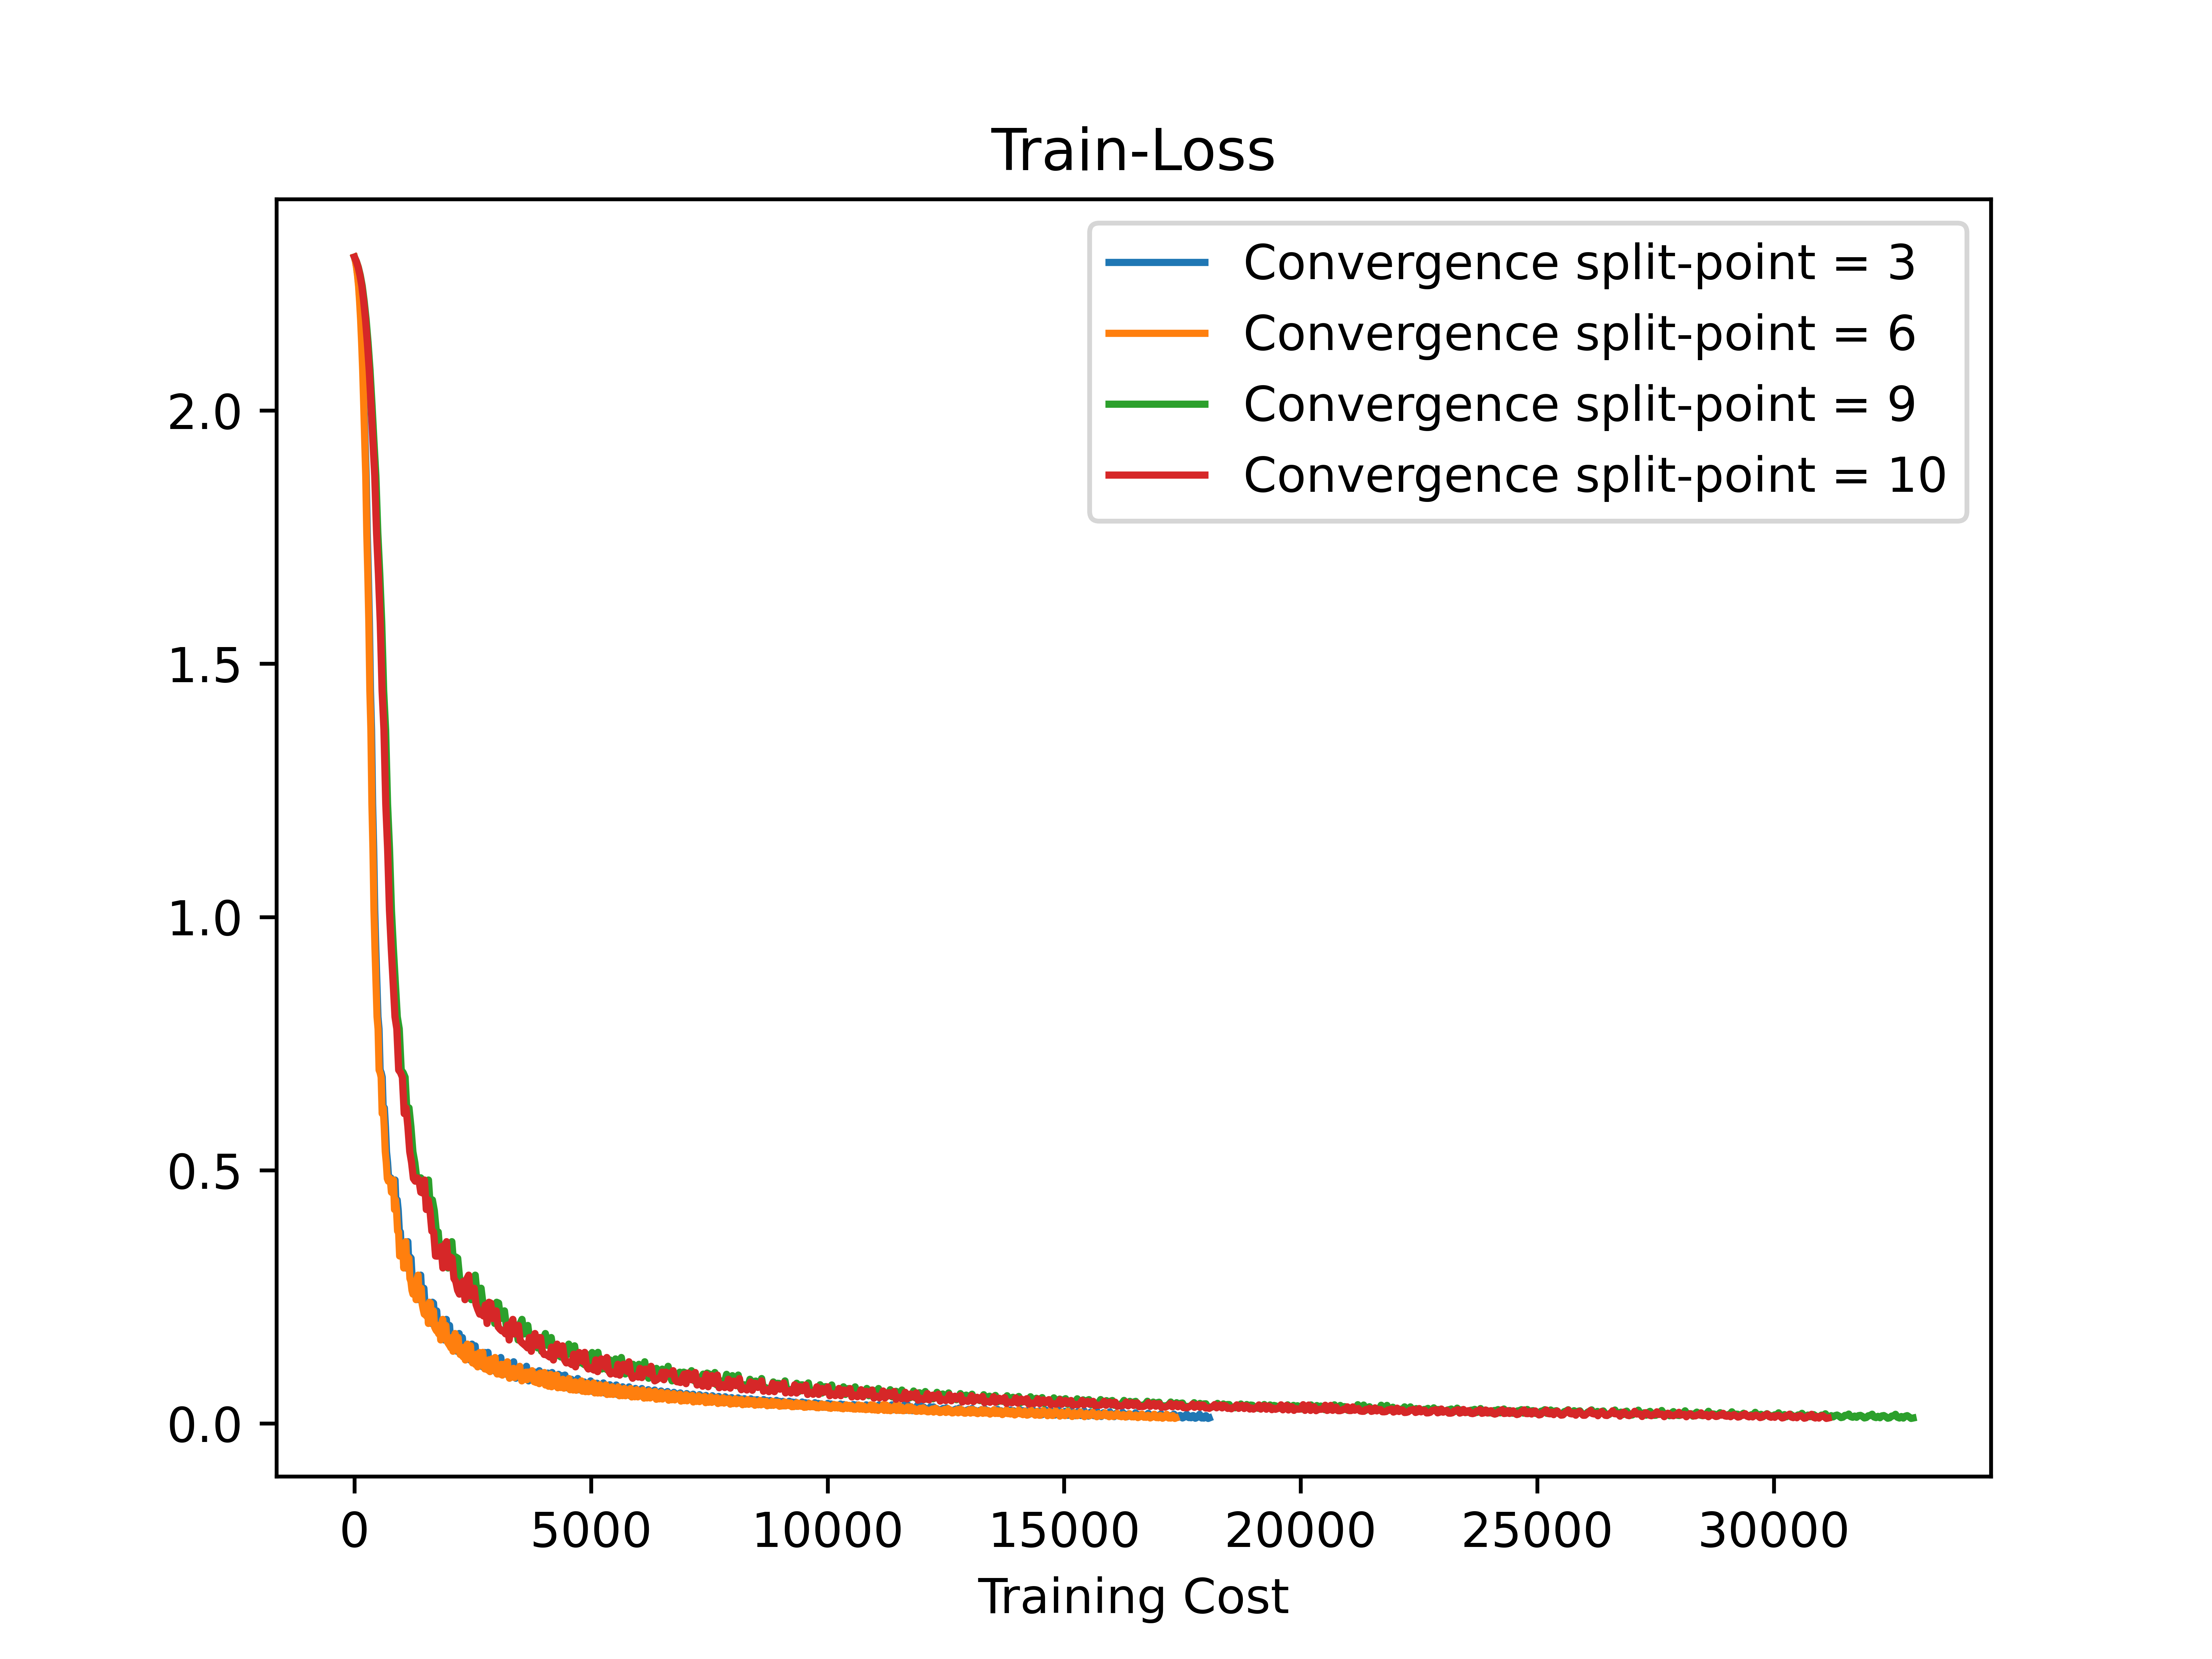
\includegraphics[width=0.45\textwidth]{pictures/Converge_Train_Loss_cost.png}
    }
    \subfigure[测试集损失]{  
        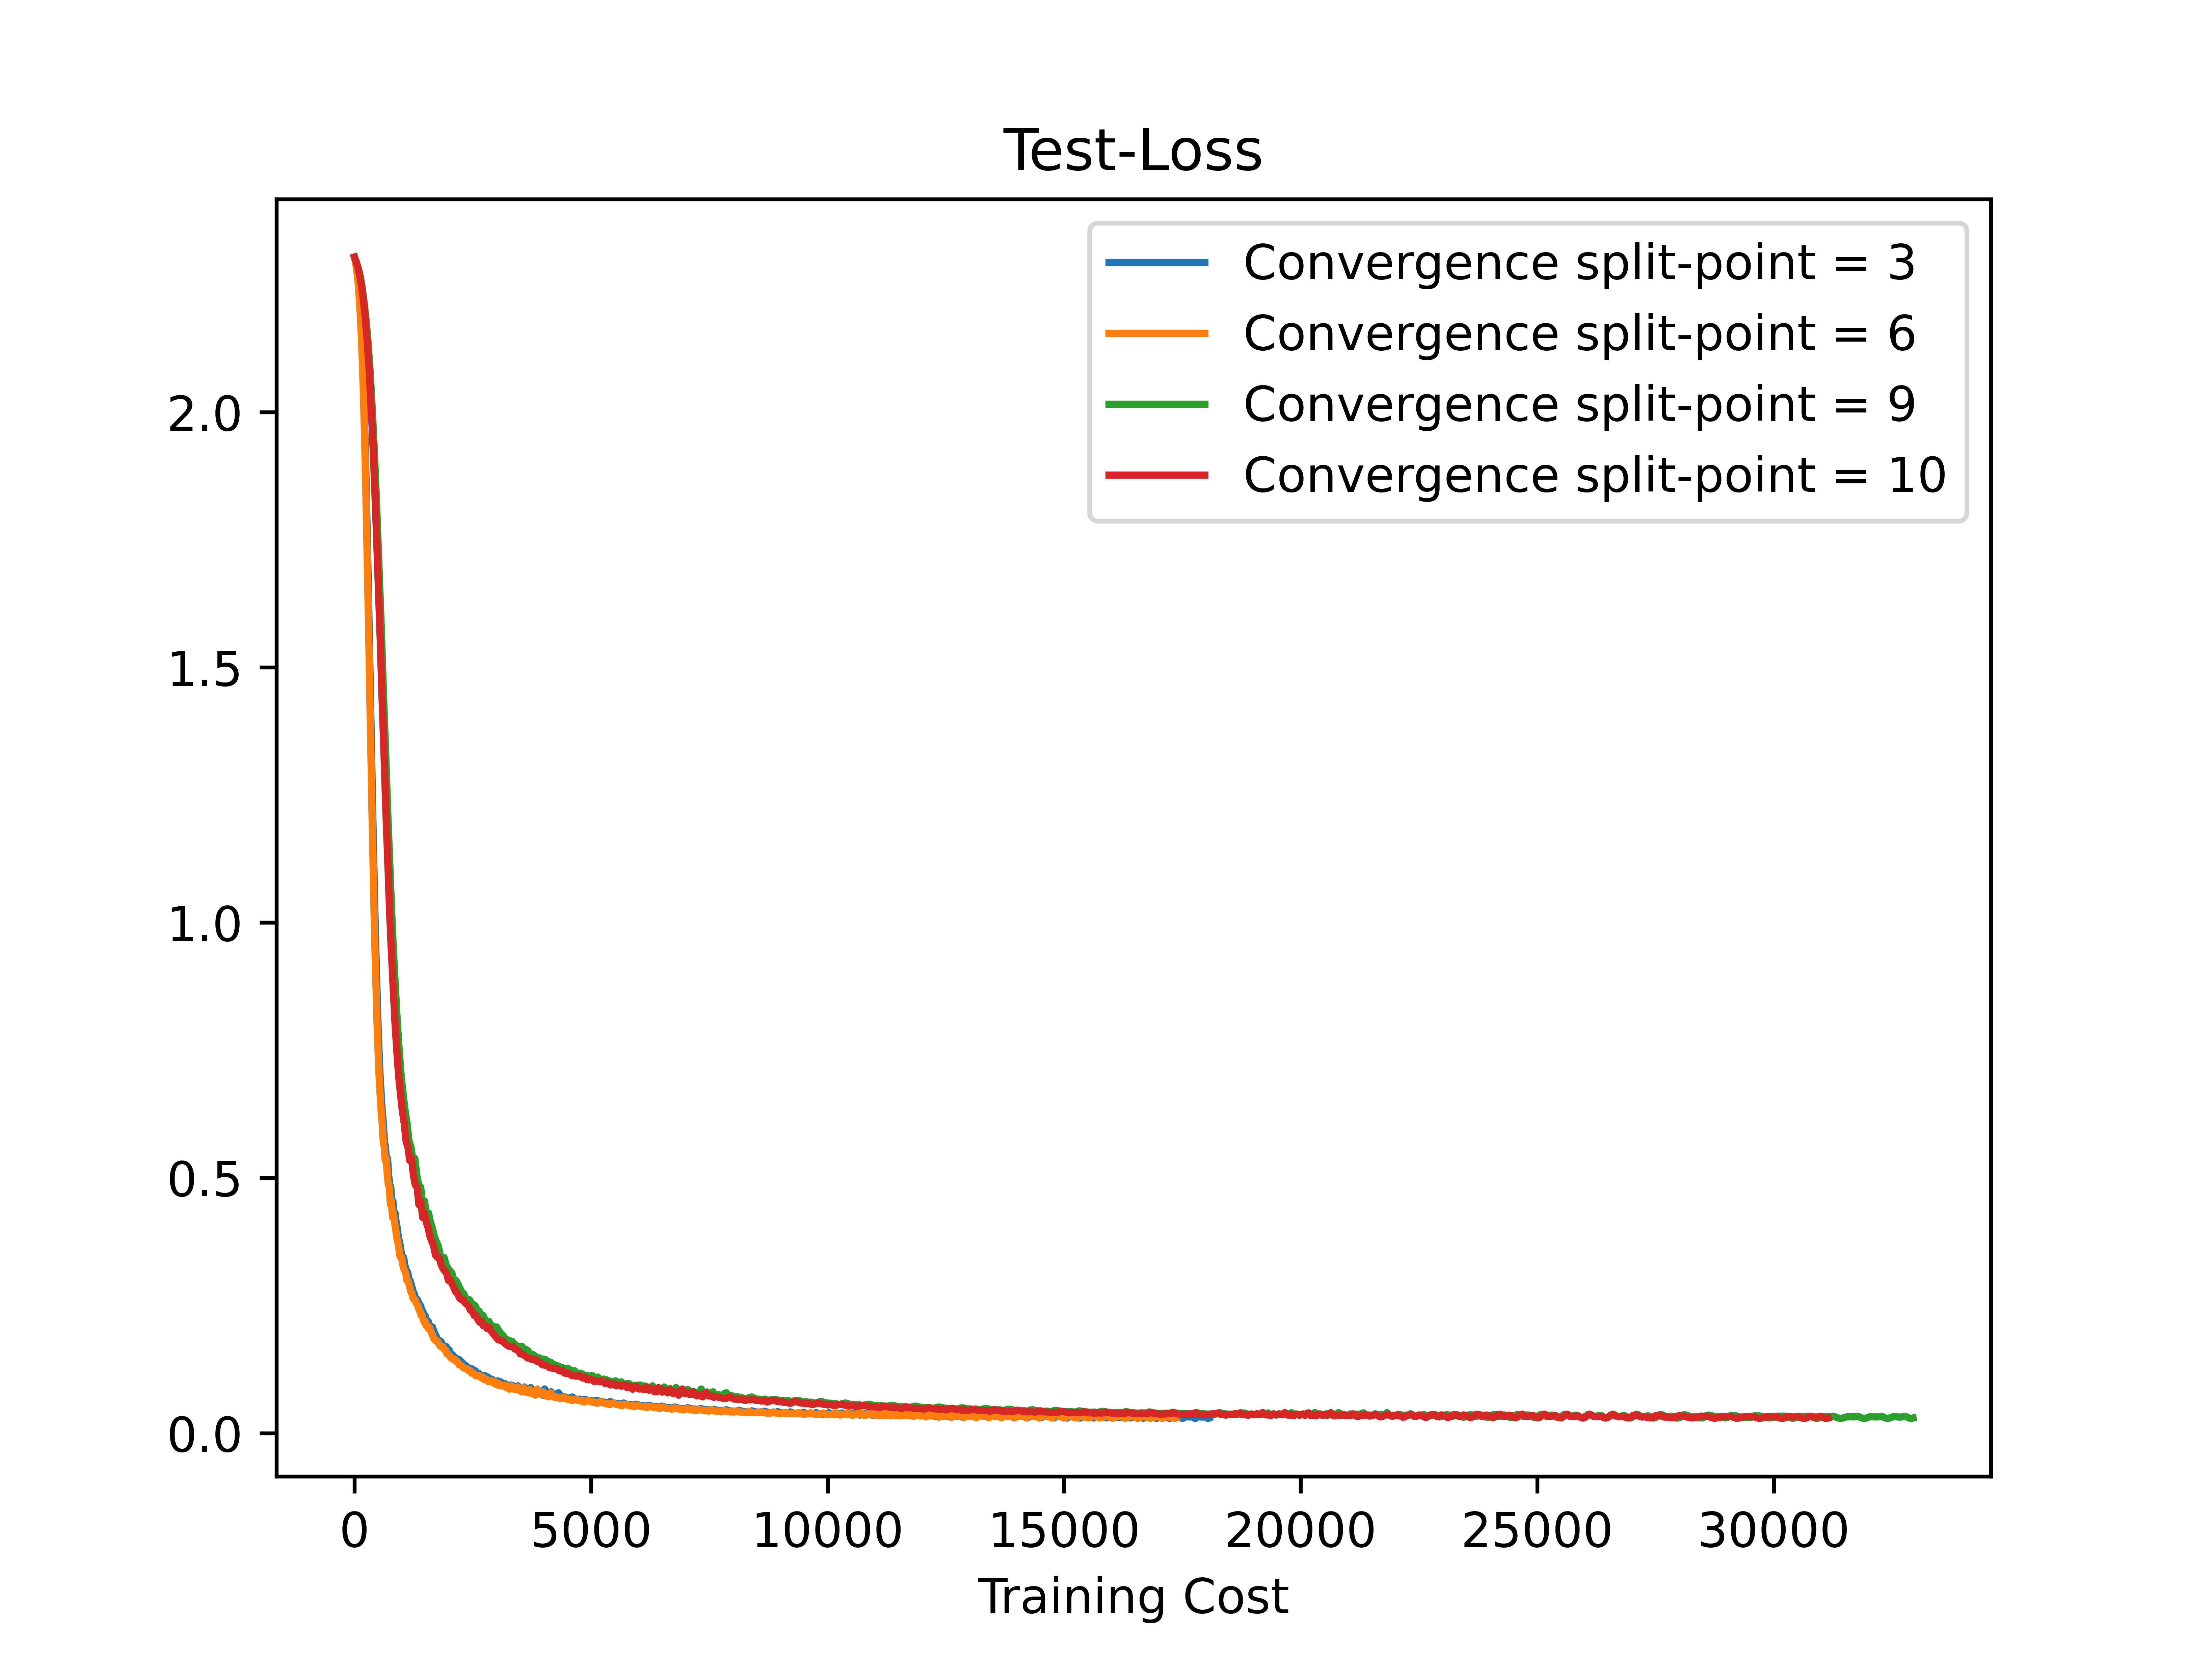
\includegraphics[width=0.45\textwidth]{pictures/Converge_Test_Loss_cost.png}
    }
    \subfigure[测试集准确率]{
        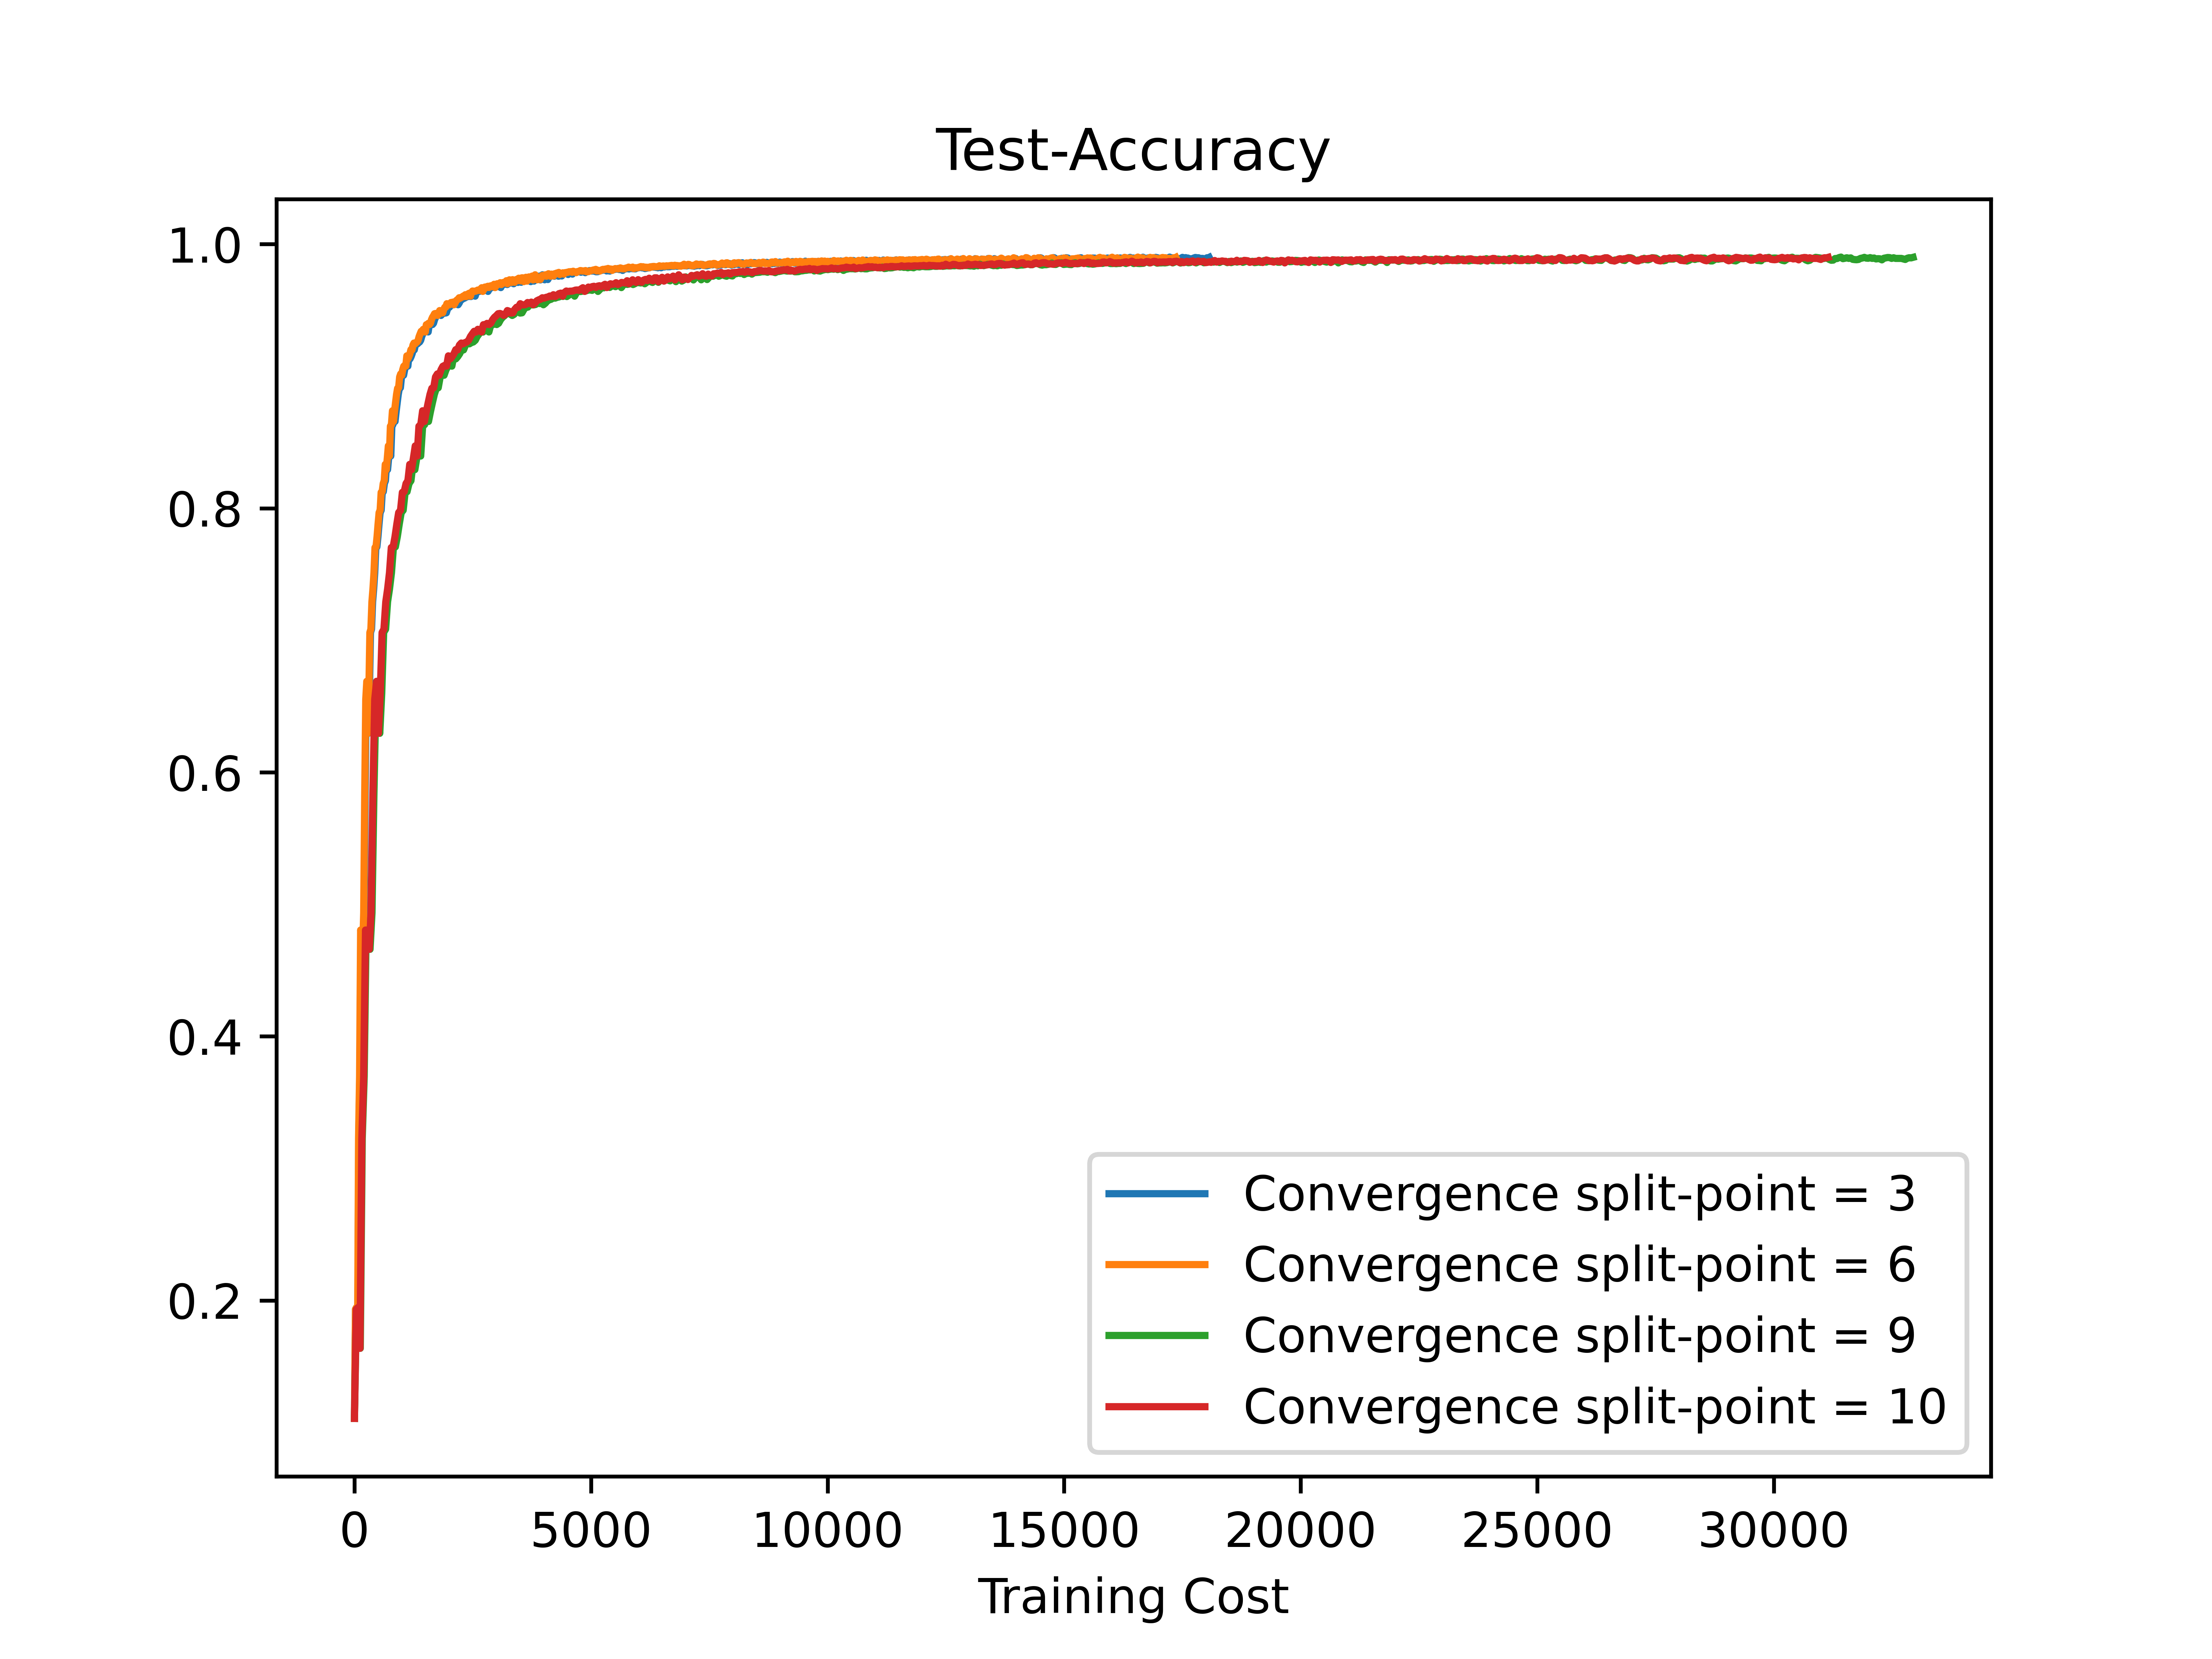
\includegraphics[width=0.45\textwidth]{pictures/Converge_Test_Accuracy_cost.png}
    }
    \caption*{图7.共享本地权重模型的训练损失,测试损失,测试准确率}
\end{figure}

从图7中可以看到,当分割点$k$为6时,的确具有最快的收敛速率,更快地达到更高的准确率和更小的损失,符合我们的预期设想。


\subsubsection{不共享本地权重模型仿真}
根据表3的训练开销,我们可以得到不共享本地权重相关的损失和准确率对于训练代价的图。

\begin{figure}[H]
    \centering
    \subfigure[训练损失]{
        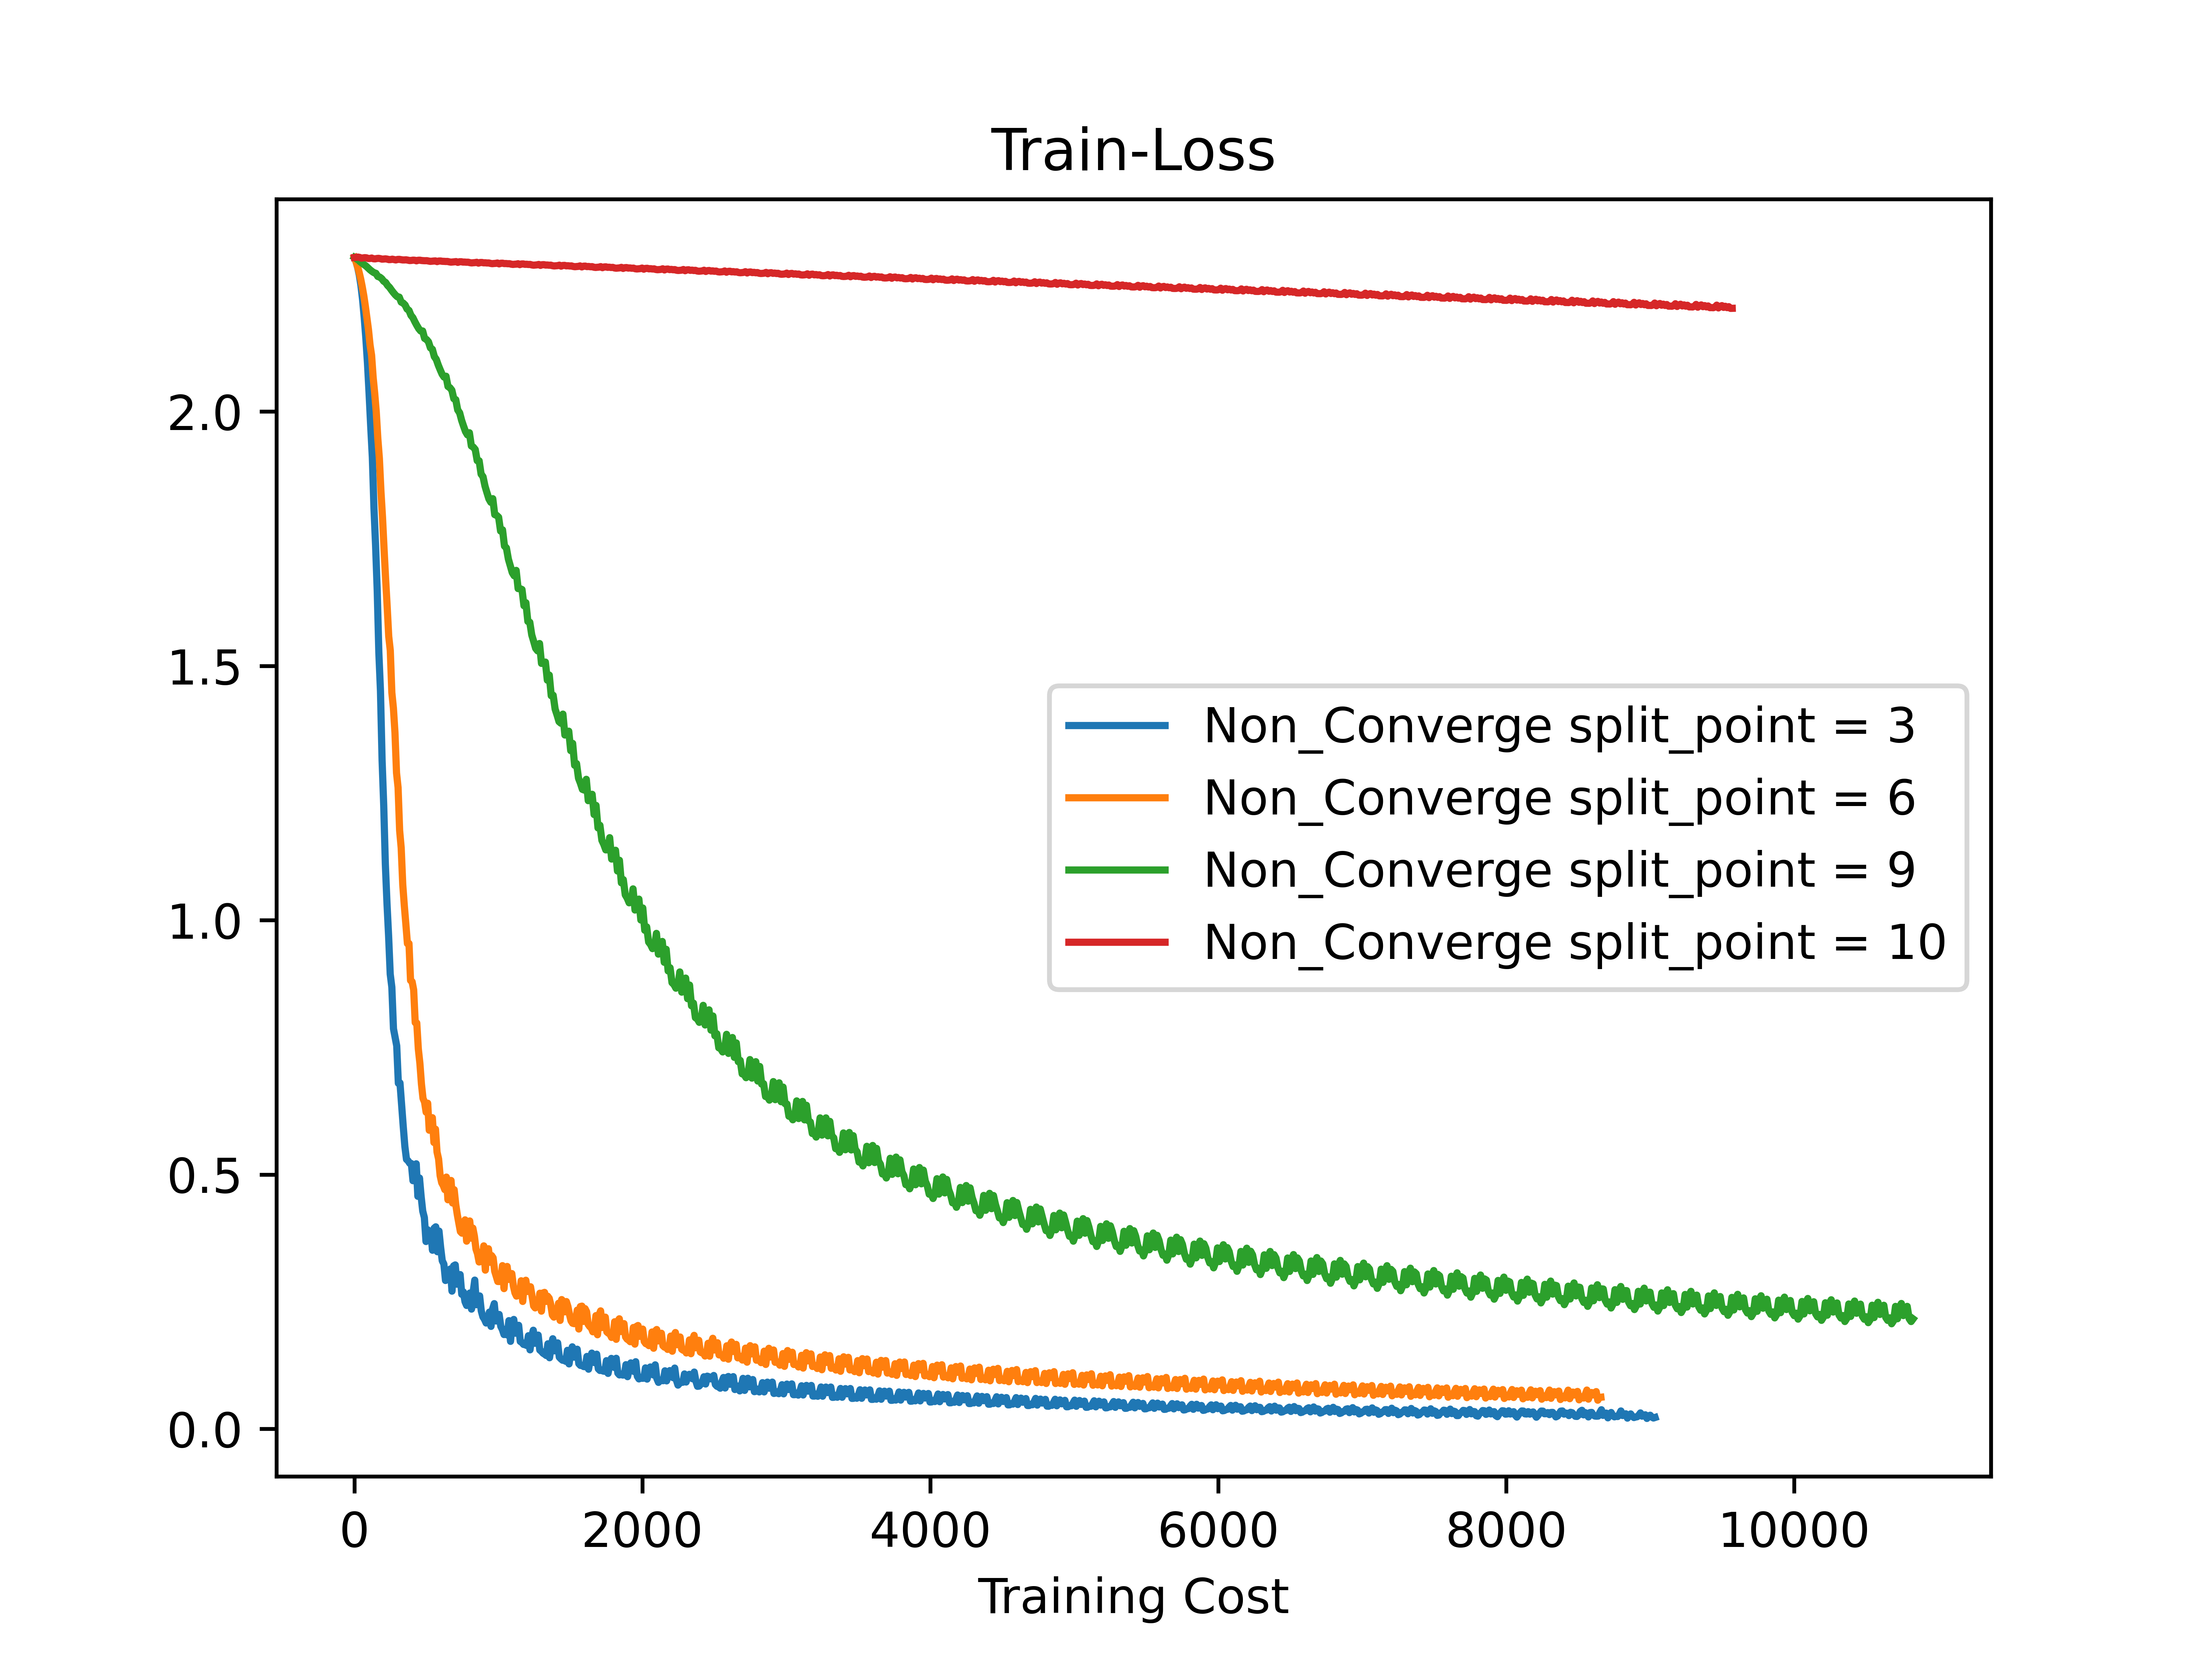
\includegraphics[width=0.45\textwidth]{pictures/Non_Converge_Train_Loss_cost.png}
    }
    \subfigure[测试集损失]{  
        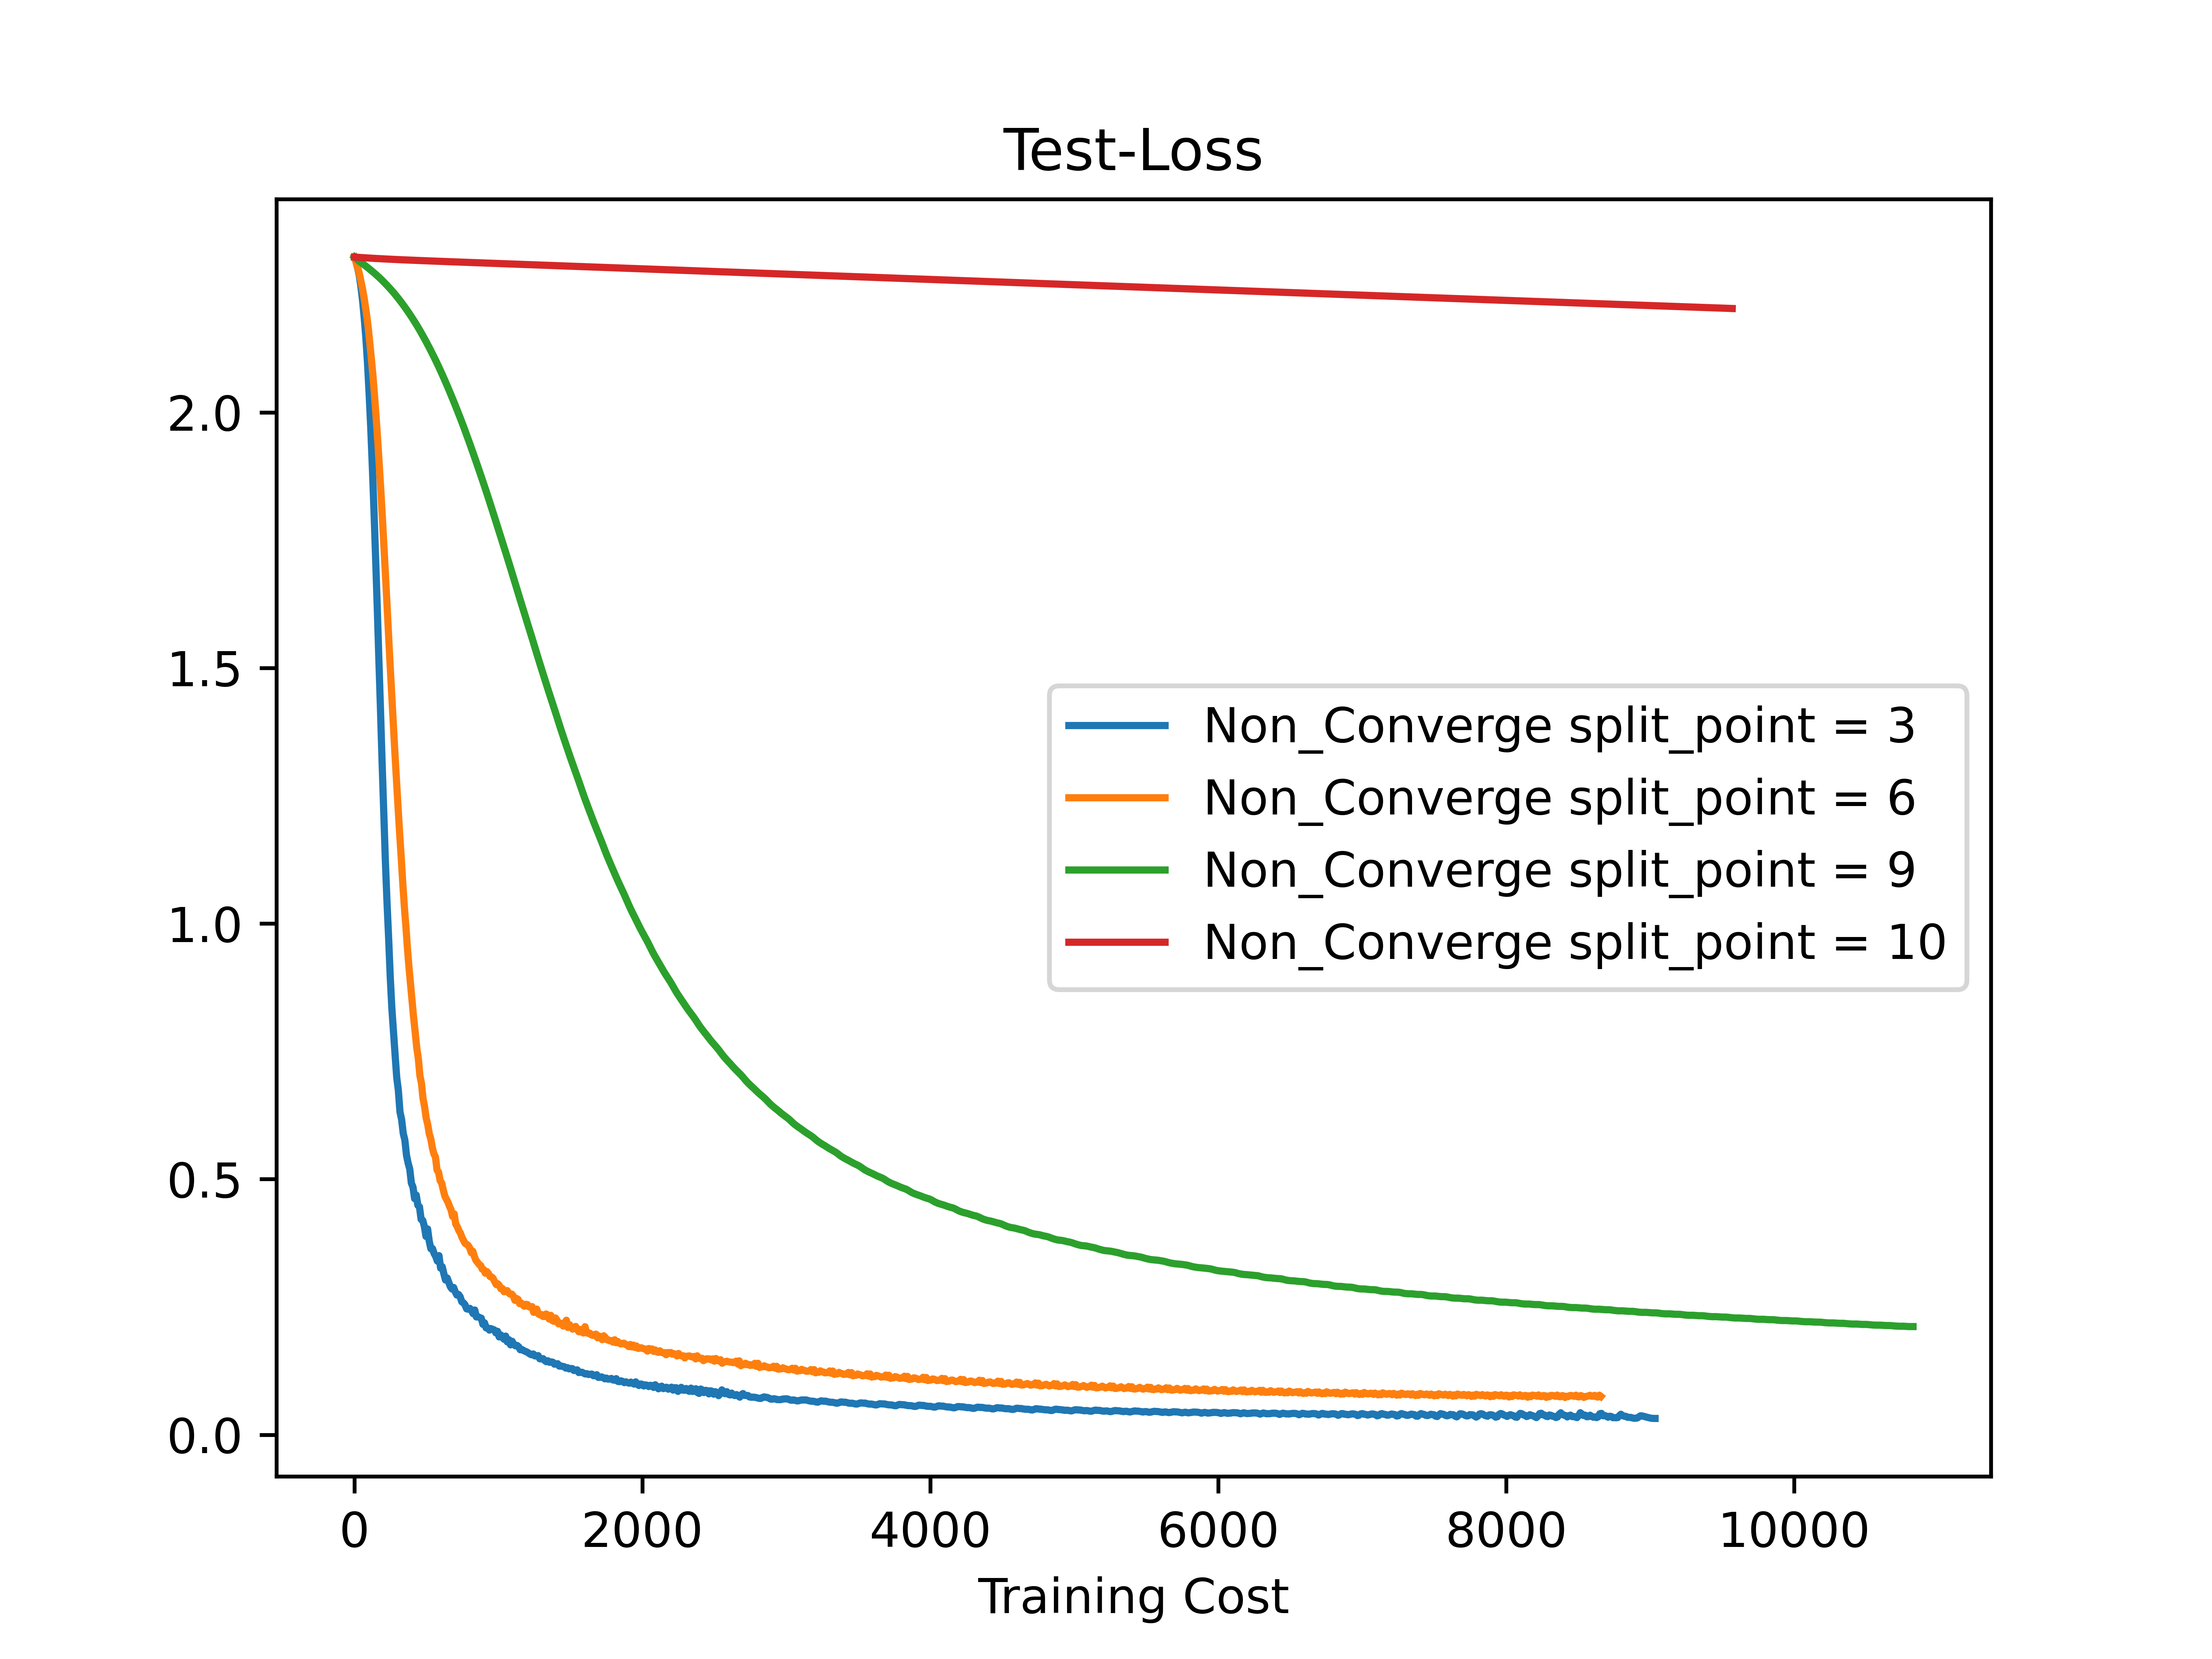
\includegraphics[width=0.45\textwidth]{pictures/Non_Converge_Test_Loss_cost.png}
    }
    \subfigure[测试集准确率]{
        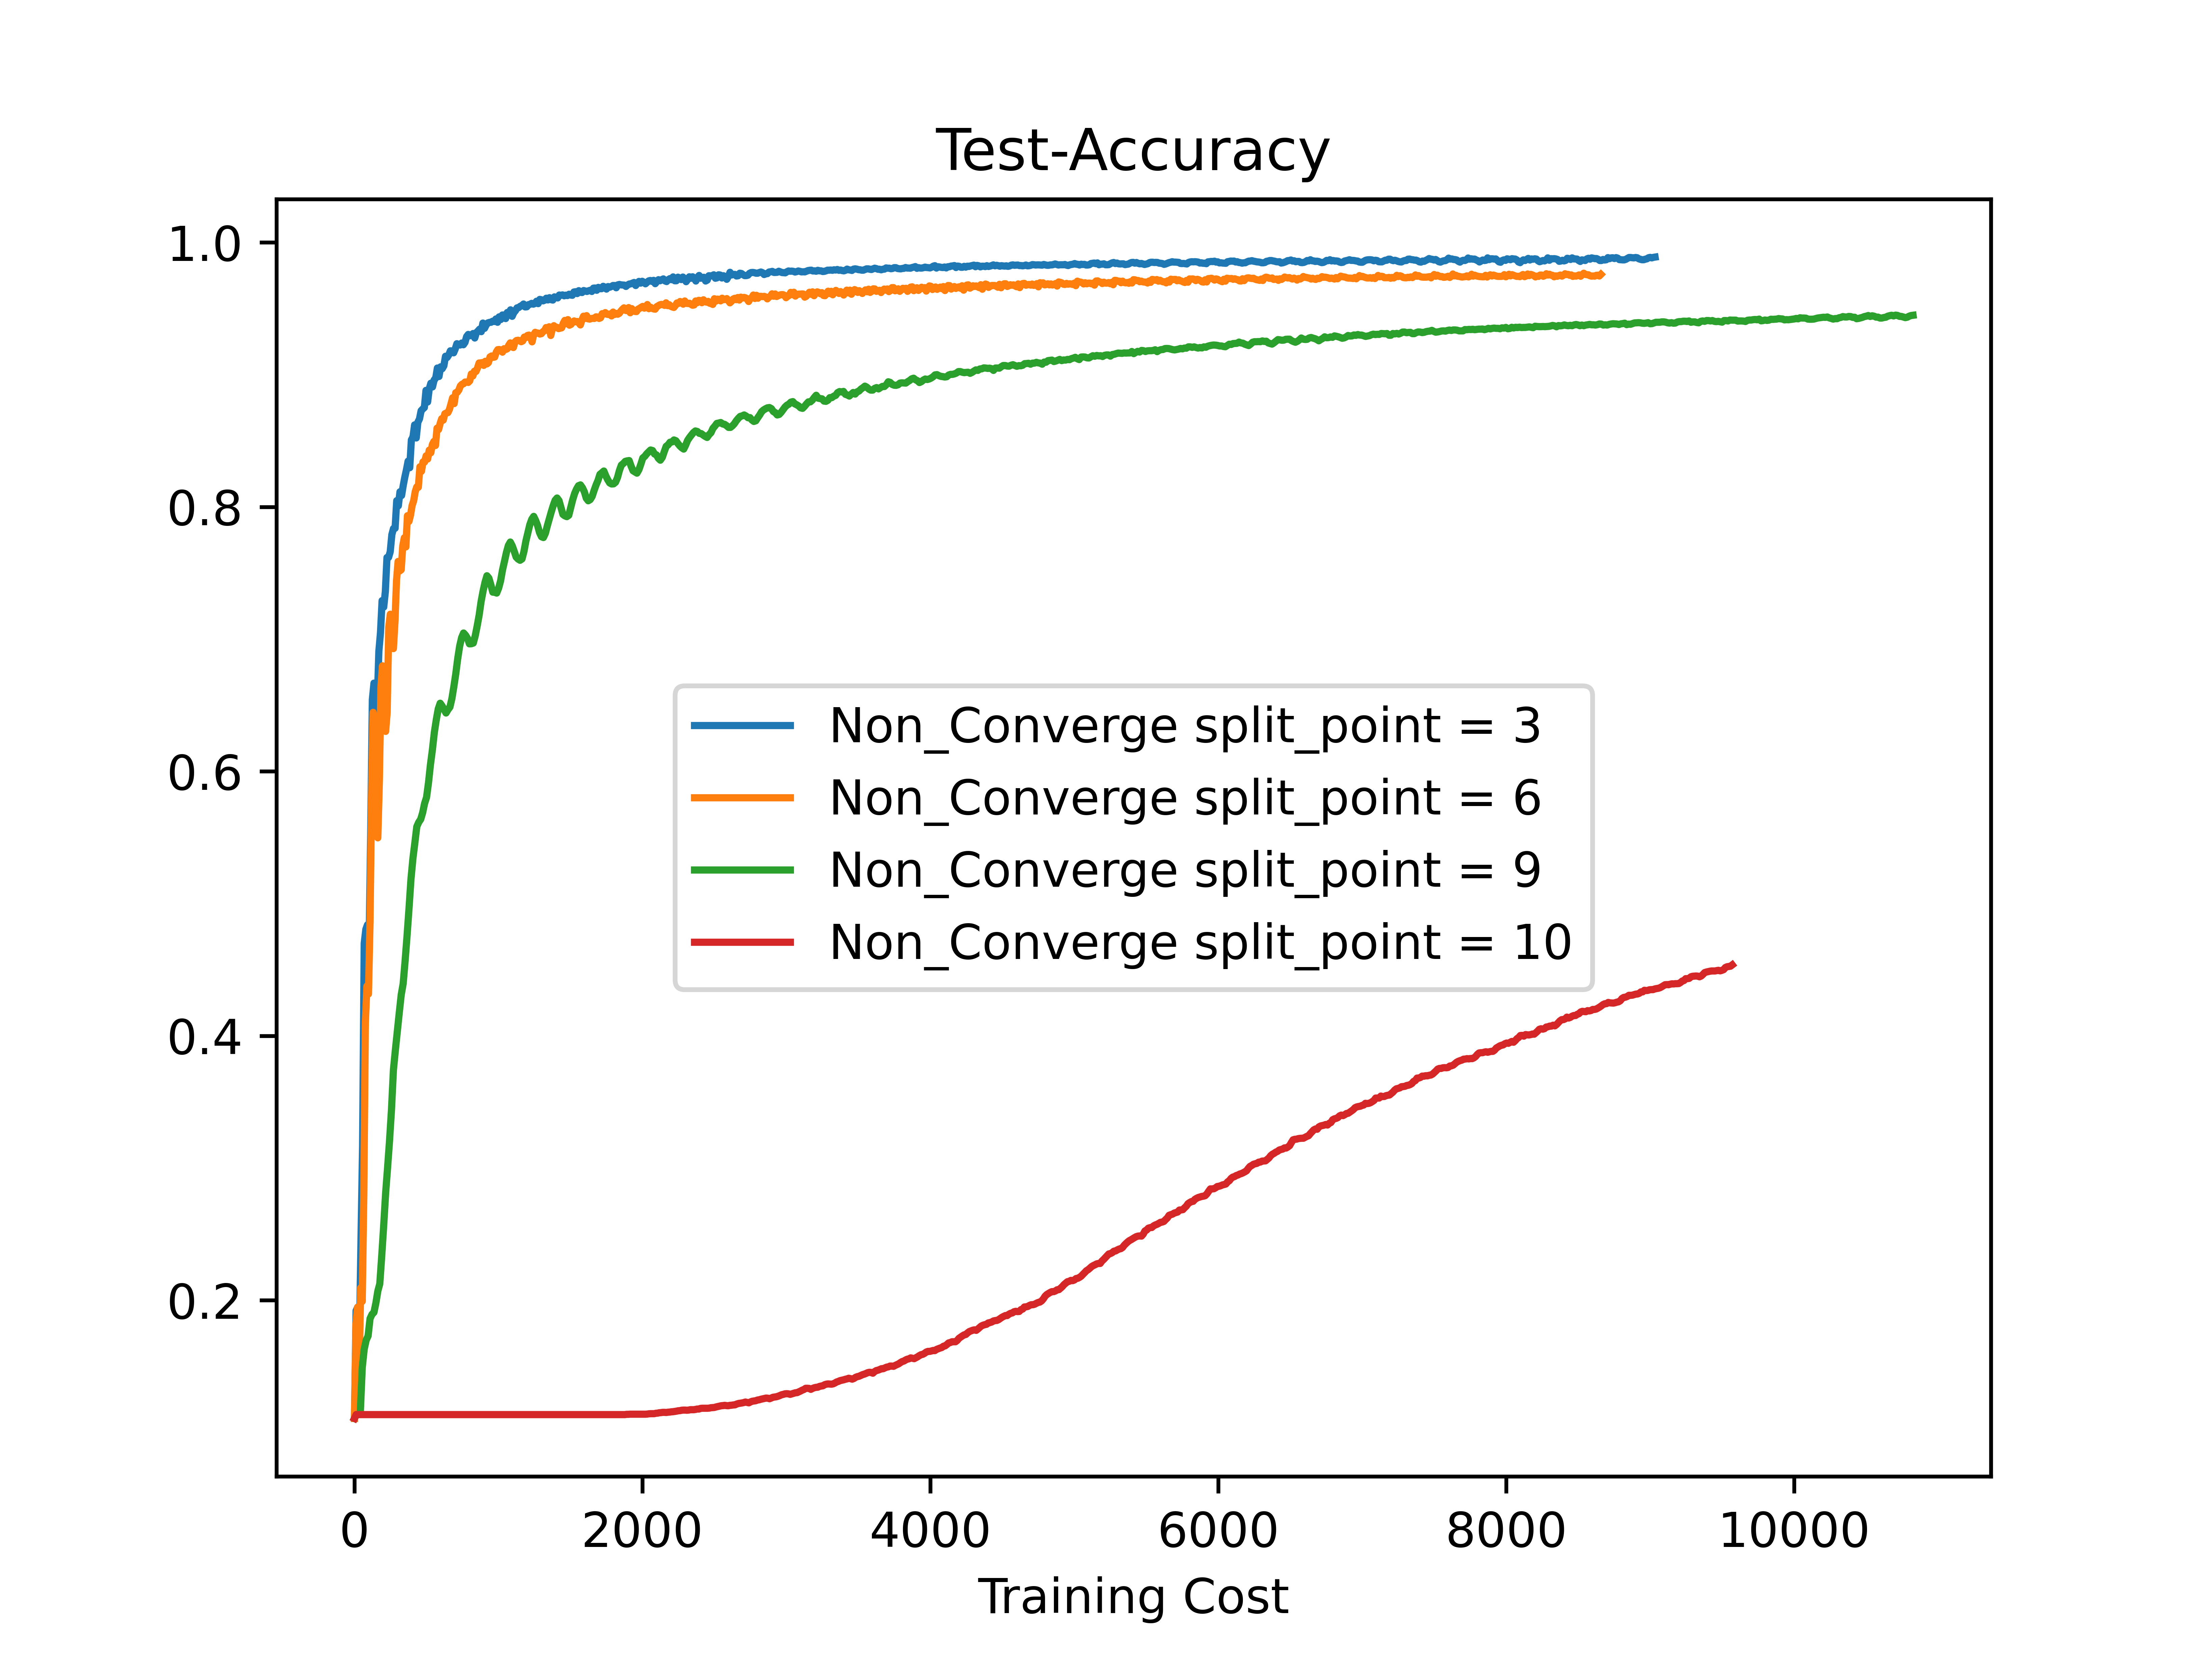
\includegraphics[width=0.45\textwidth]{pictures/Non_Converge_Test_Accuracy_cost.png}
    }
    \caption*{图8.不共享本地权重模型的训练损失,测试损失,测试准确率}
\end{figure}

从图8中可以看到,之前根据训练开销最小化计算出的分割点为$6$,在图中有不错的准确率和损失,准确率也高于$92\%$。
虽然牺牲了部分模型,但是也达到了比较好的结果。

同时,当分割点$k=3$时,收敛效果最好,但是对于训练开销来说,分割点为$6$时是最小的,但是两者相差无几。

在训练之前,是并不知道训练结果和准确率,因此,对于不共享本地权重的模型,本文认为,不仅要考虑训练开销,还需要分割点在学习模型的前面几层。
分割点层数越靠前,牺牲的模型越少,准确率也会相应的提高。

\subsubsection{三种模型仿真结果比较}
根据表3的训练开销以及上述测试,我们发现分割点$k=6$时,共享本地权重模型与不共享本地权重模型都可以达到最⼩的训练开销,因此我们使⽤该分
割点来⽐较两种模型分割机制的具体训练开销。
\begin{figure}[H]
    \centering
    \subfigure[训练损失]{
        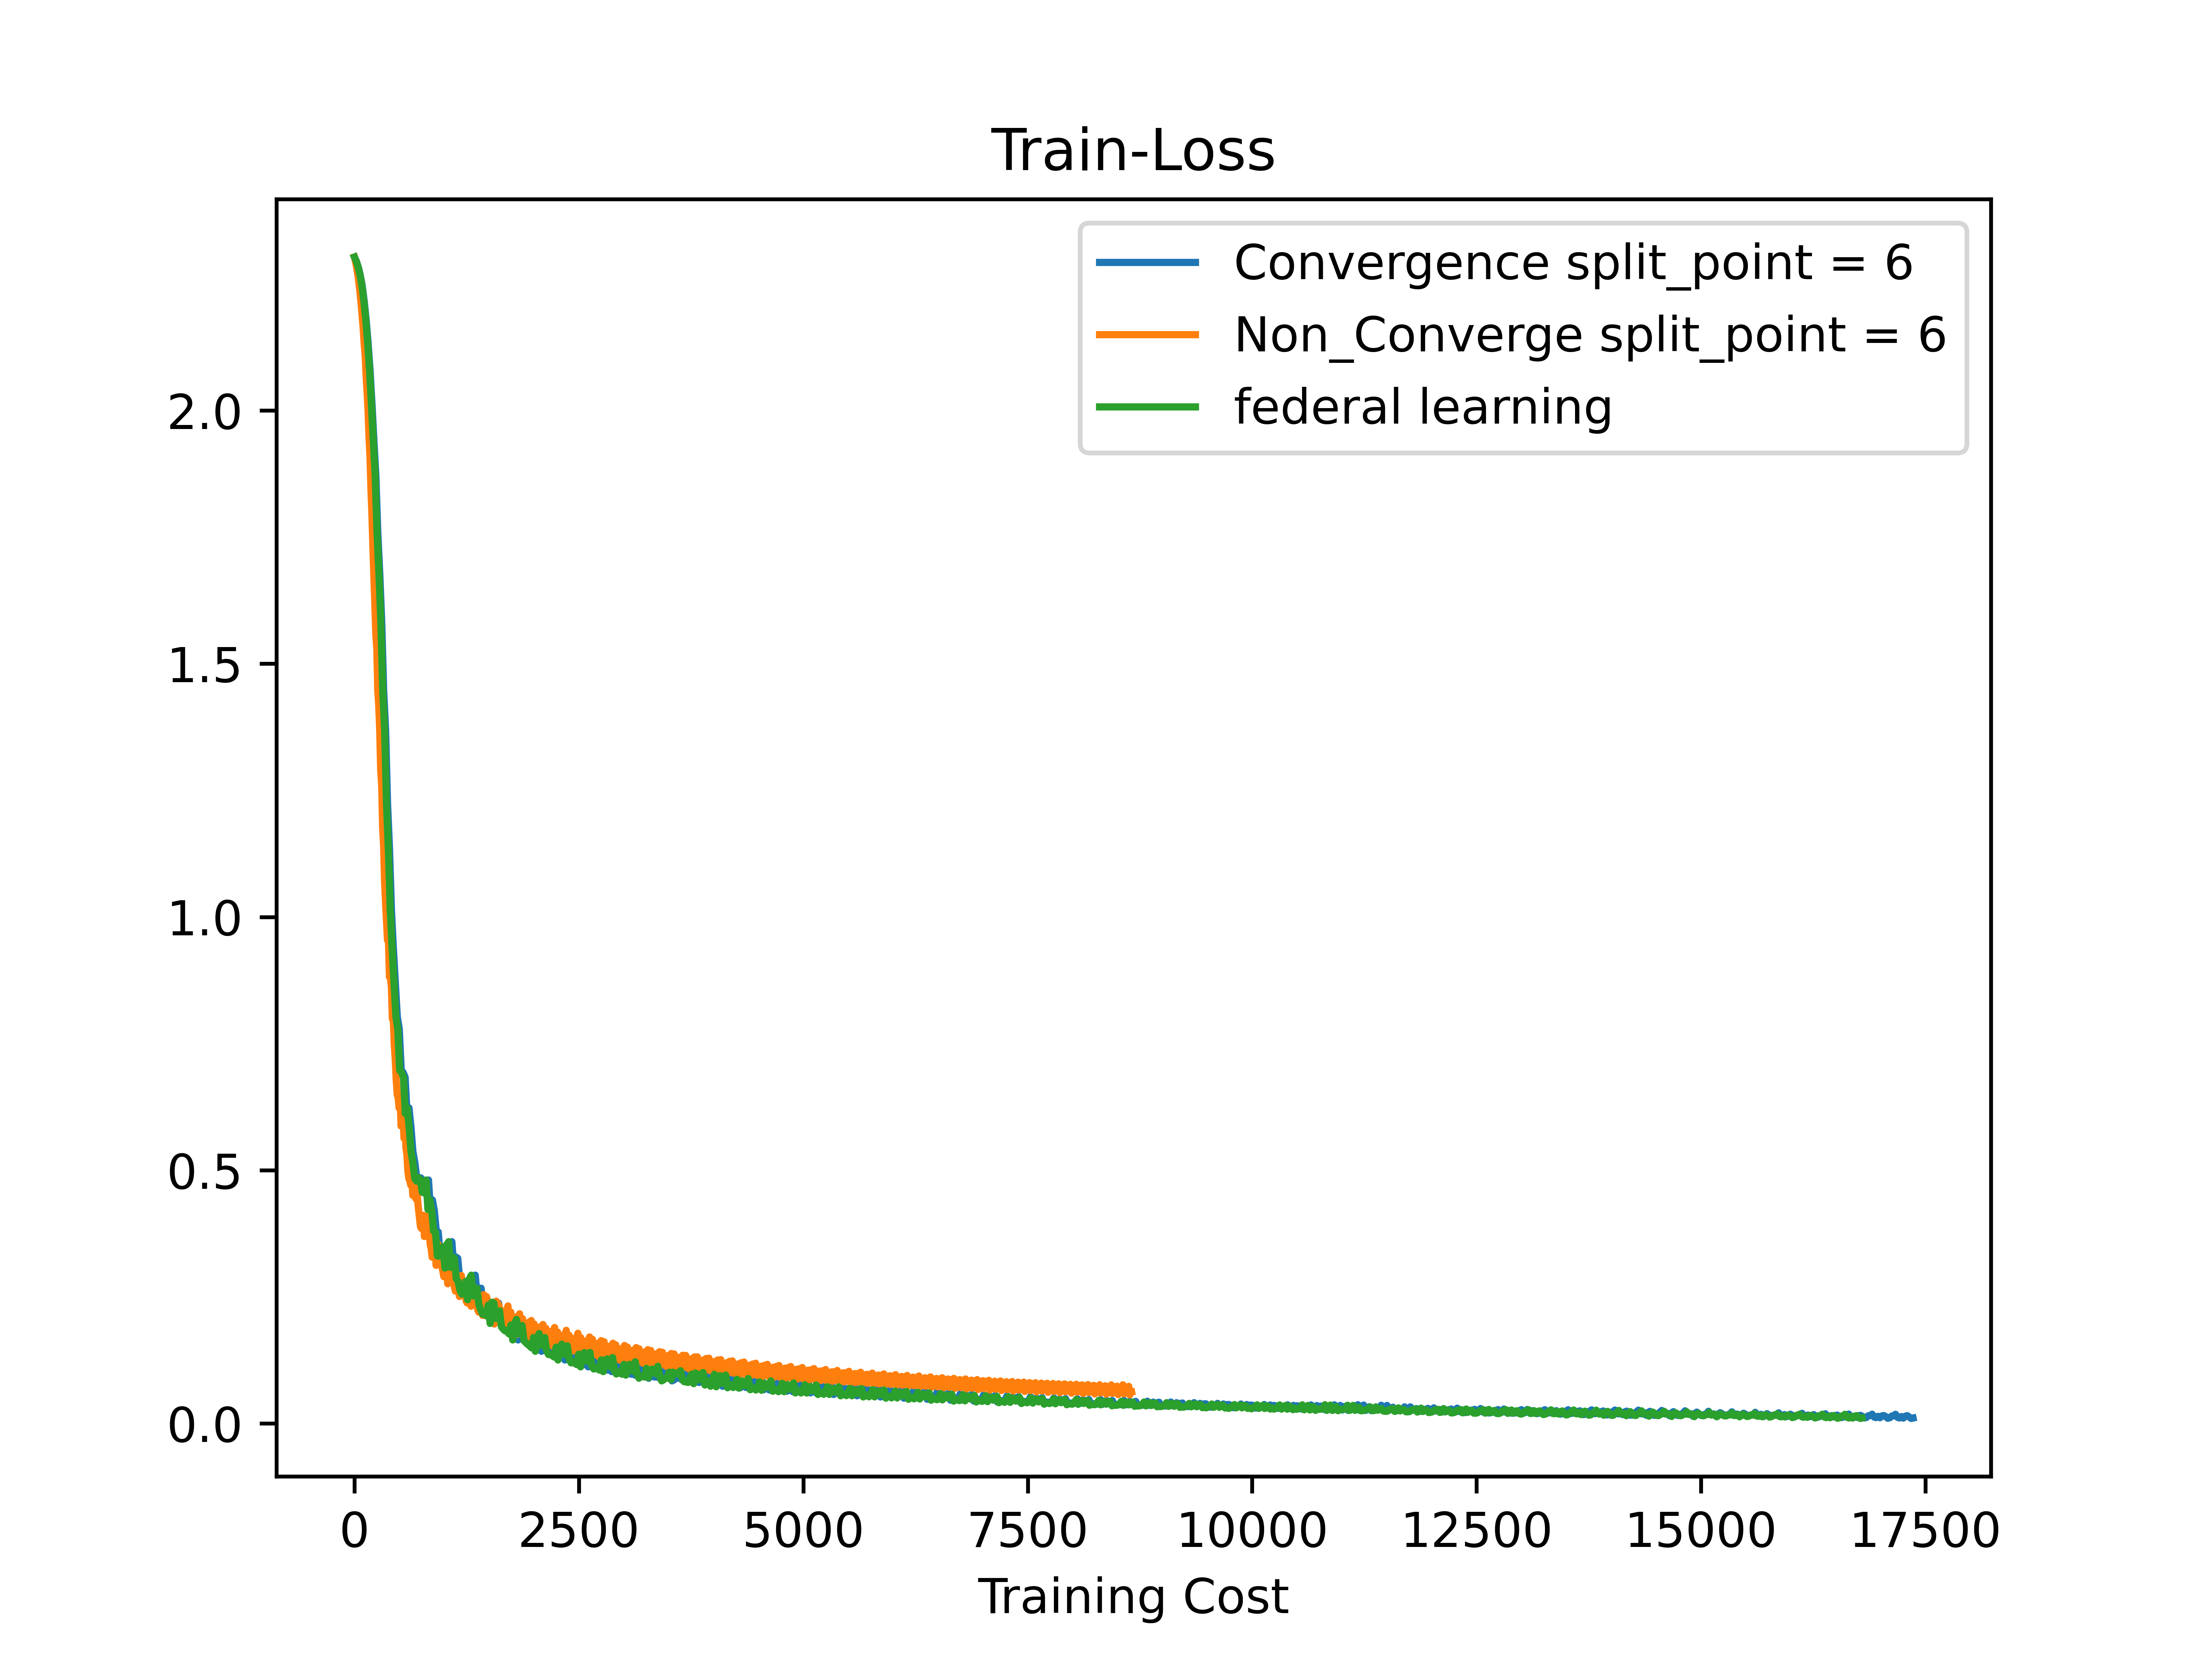
\includegraphics[width=0.45\textwidth]{pictures/kinds3_Train_Loss_cost.png}
    }
    \subfigure[测试集损失]{  
        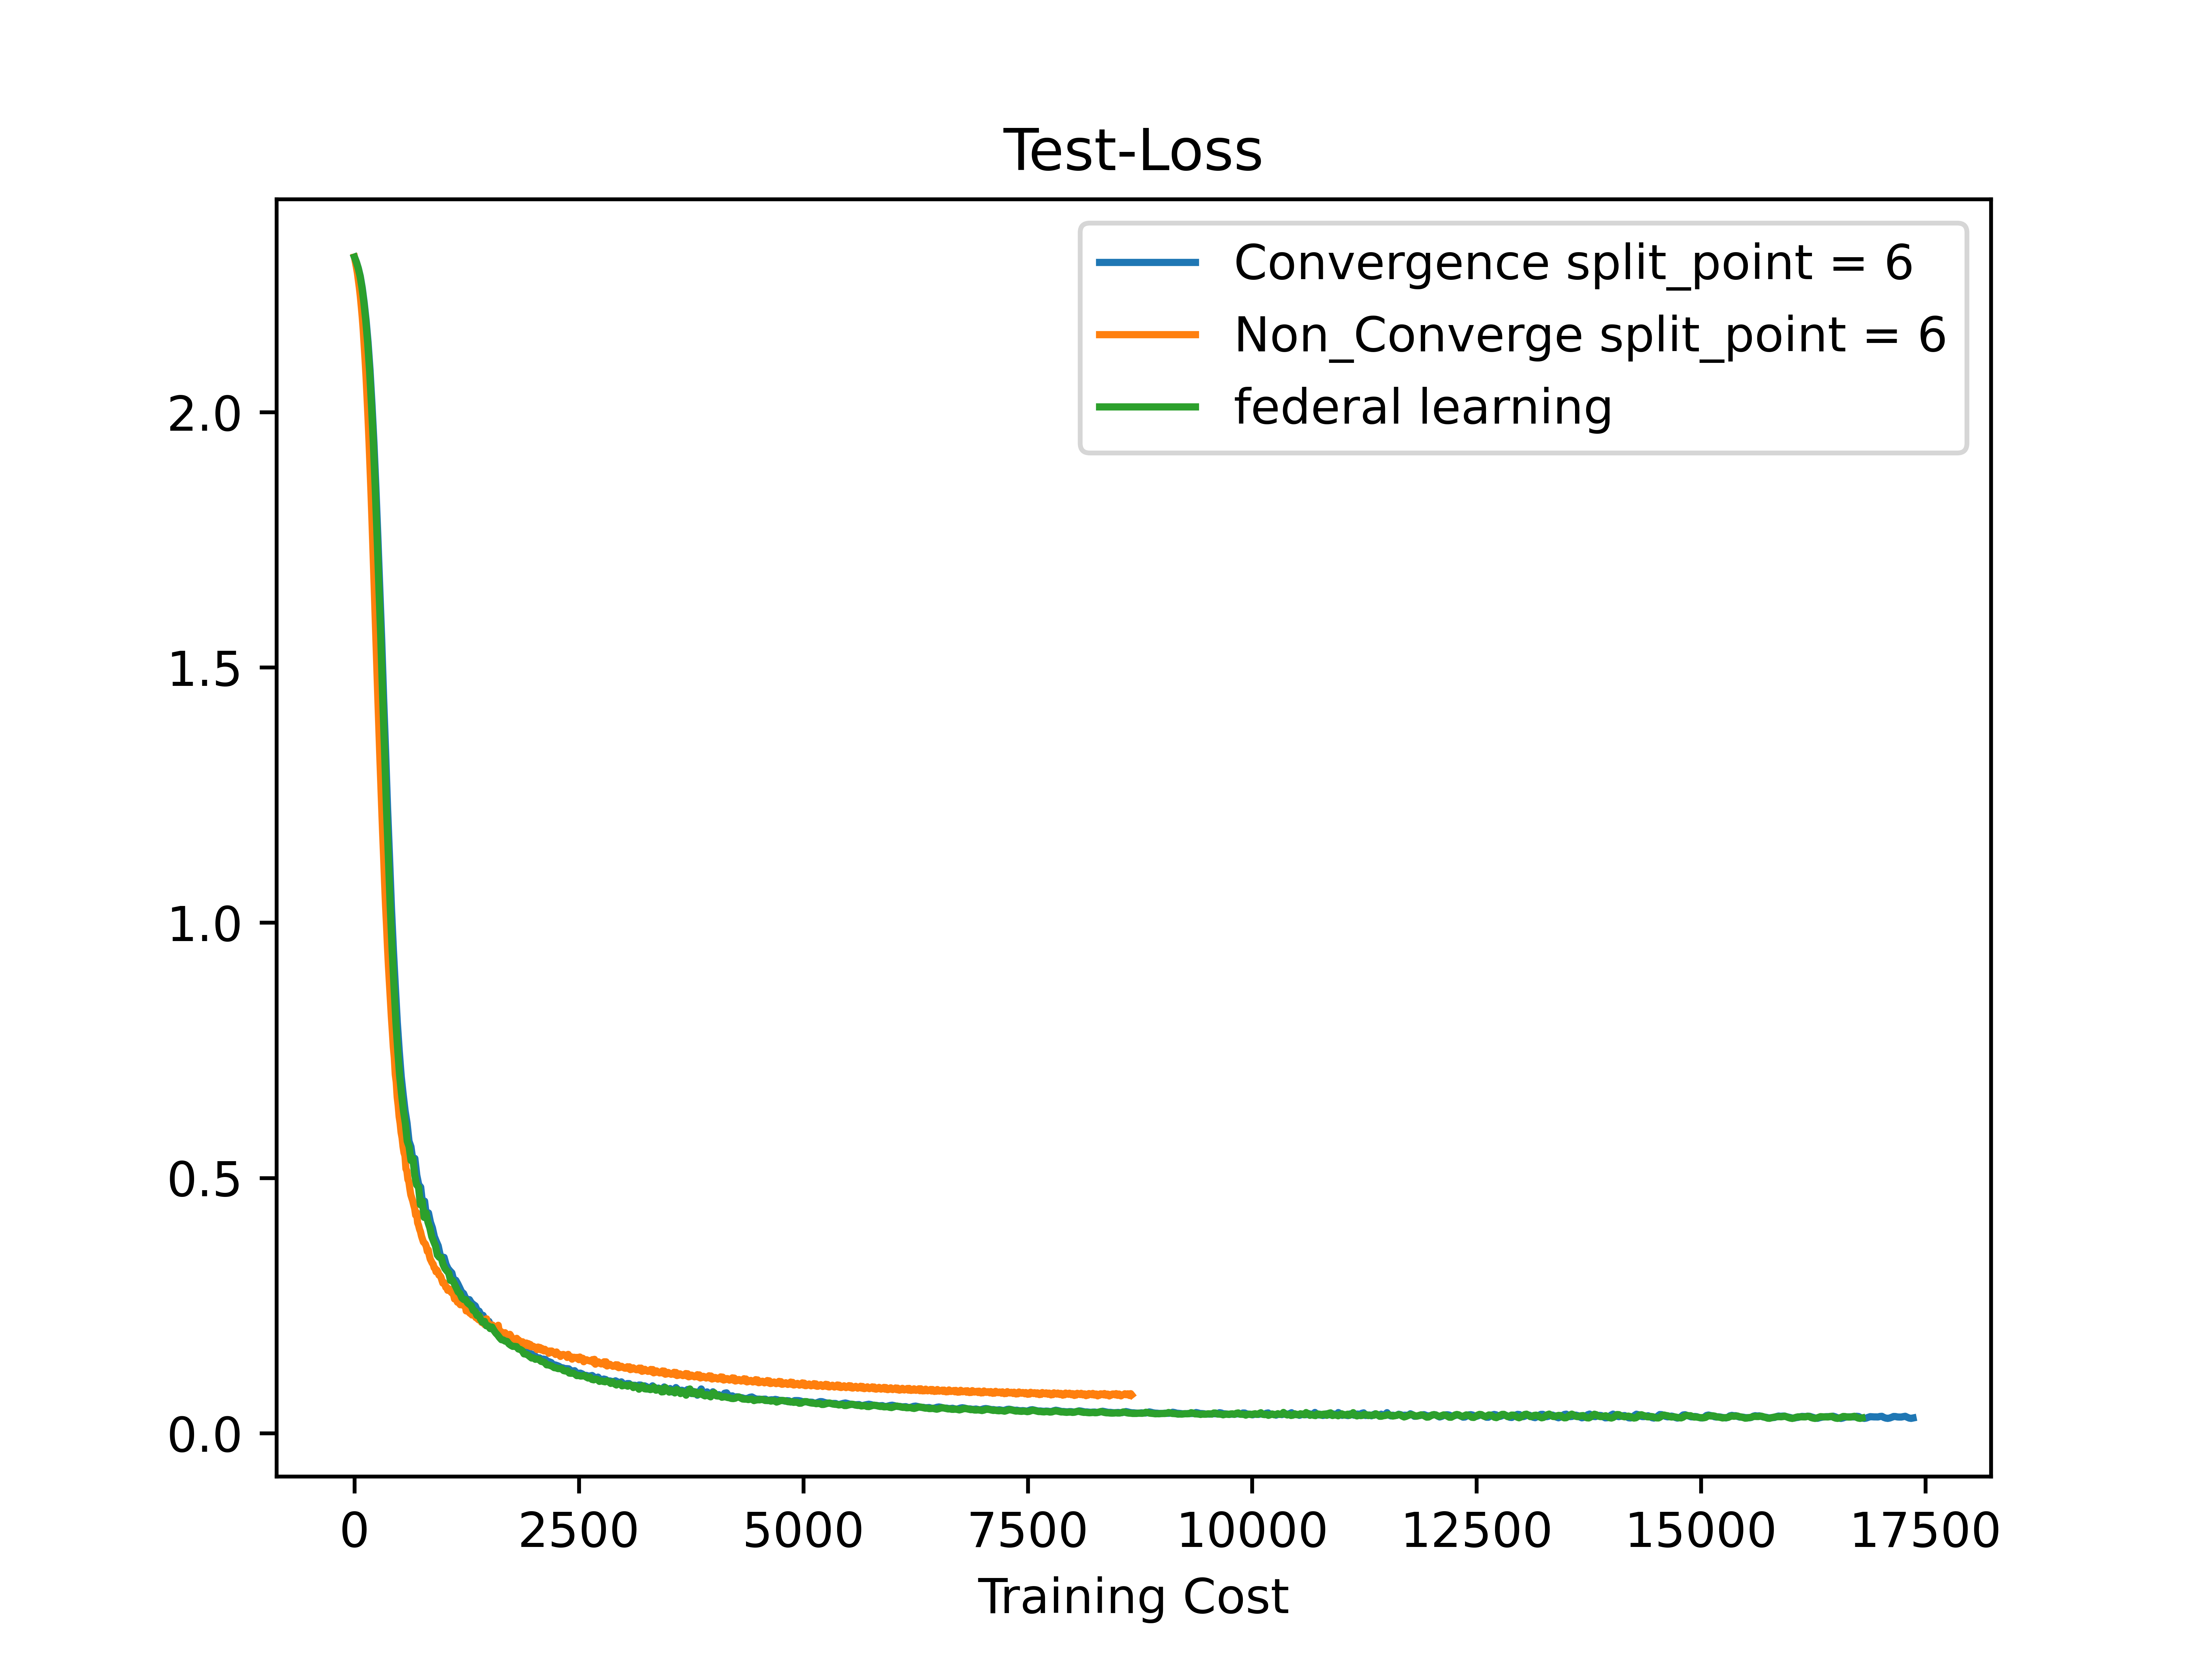
\includegraphics[width=0.45\textwidth]{pictures/kinds3_Test_Loss_cost.png}
    }
    \subfigure[测试集准确率]{
        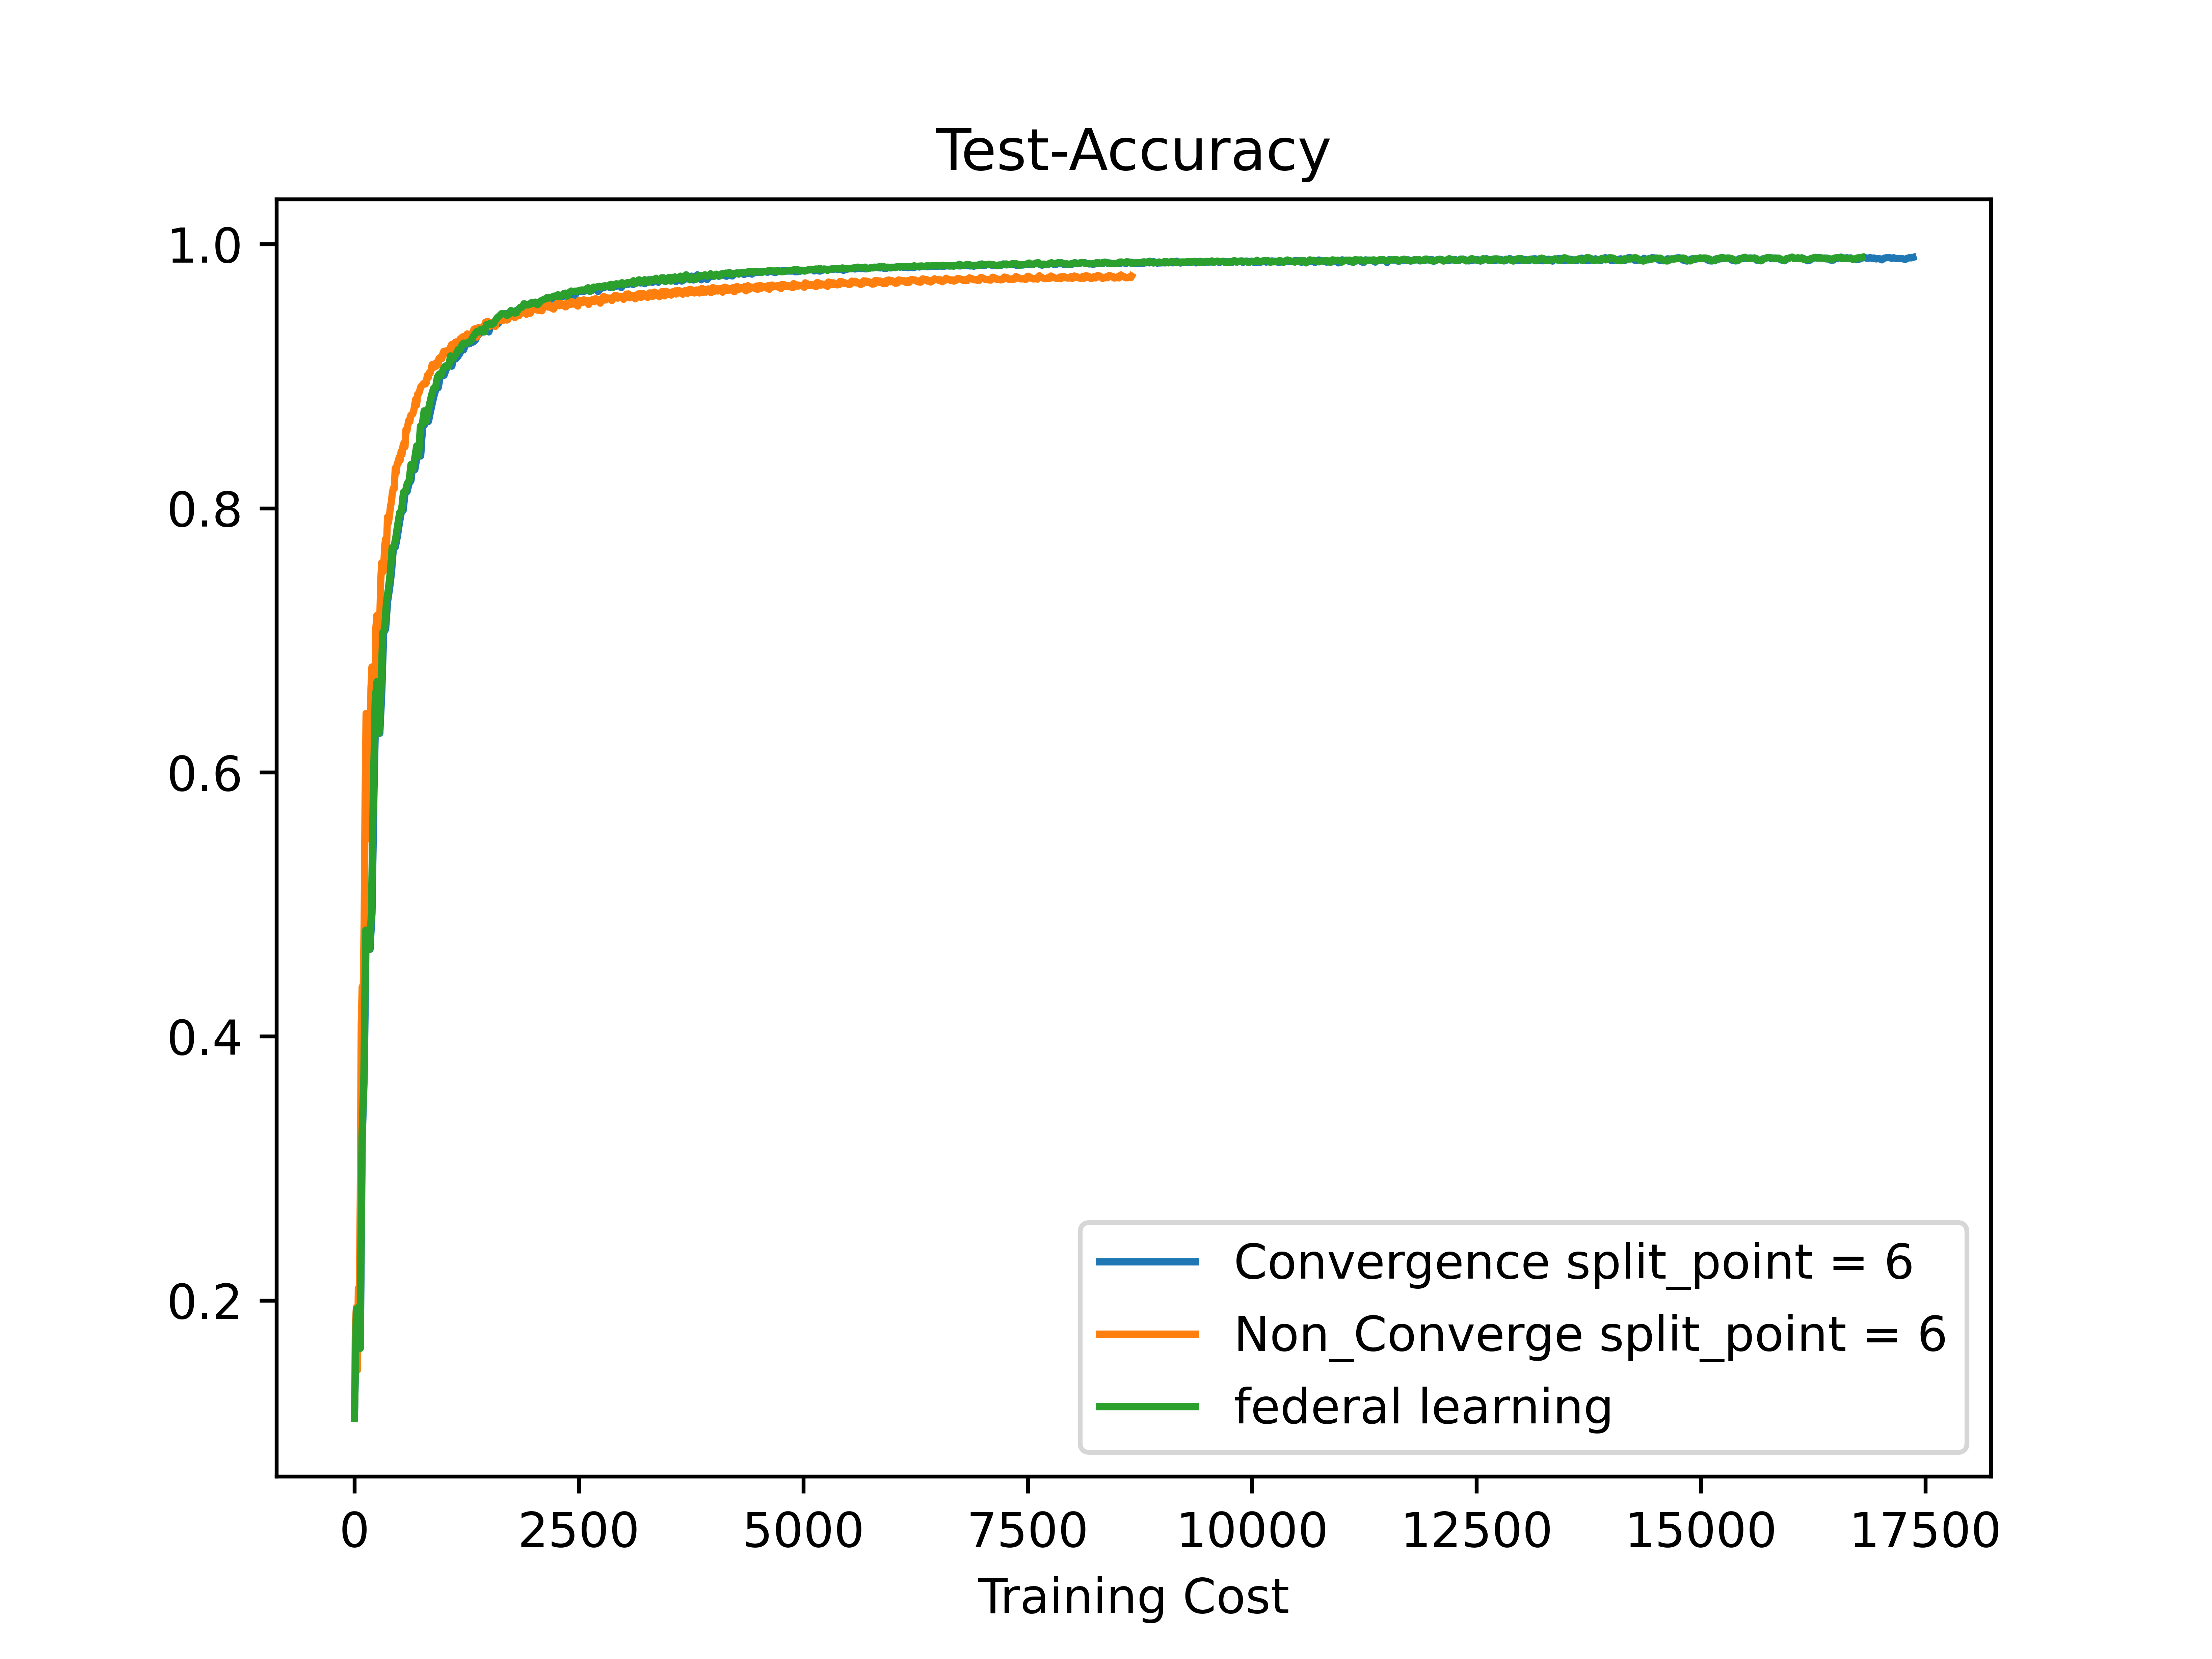
\includegraphics[width=0.45\textwidth]{pictures/kinds3_Test_Accuracy_cost.png}
    }
    \caption*{图9.三种模型仿真结果比较}
\end{figure}

很明显,在图9当中,三条曲线有交汇,这表明了,在交汇点之前,不共享本地权重的模型具有更快的收敛效率,之后随着训练开销增大,准确率以及损失会被不共享本地权重的模型和传统联邦学习模型赶上。
因此,在训练开销较小的情况下,不共享本地权重的模型具有一定优势,比如更快到达收敛,节约了时间成本、计算成本以及传输成本等。

对于共享本地权重模型和传统联邦学习模型,两者训练开销相似,共享本地权重模型开销稍微比传统联邦学习大,因此在图中基本重合。
但是也可以预测到,如果学习模型中间有节点较少而且比较靠前时,共享本地权重模型在该点为分割点的开销会大幅减小。

\section{实物测试}

根据仿真,笔者也搭建了一套实物的仿真平台,如图10所示。我们这里使用了三个终端设备,分别是一个树莓派、一个Jetson Nano、以及一个个人电脑,并且以另一台电脑当作服务器。
服务器和各个终端之间通过TCP连接,互相传递数据信息。
于此同时,我们在服务器上绘制了一个图形界面,可以时时看到每次迭代的损失,以及测试的损失和准确率,并绘制出图形来。

\begin{figure}[H]
    \centering
    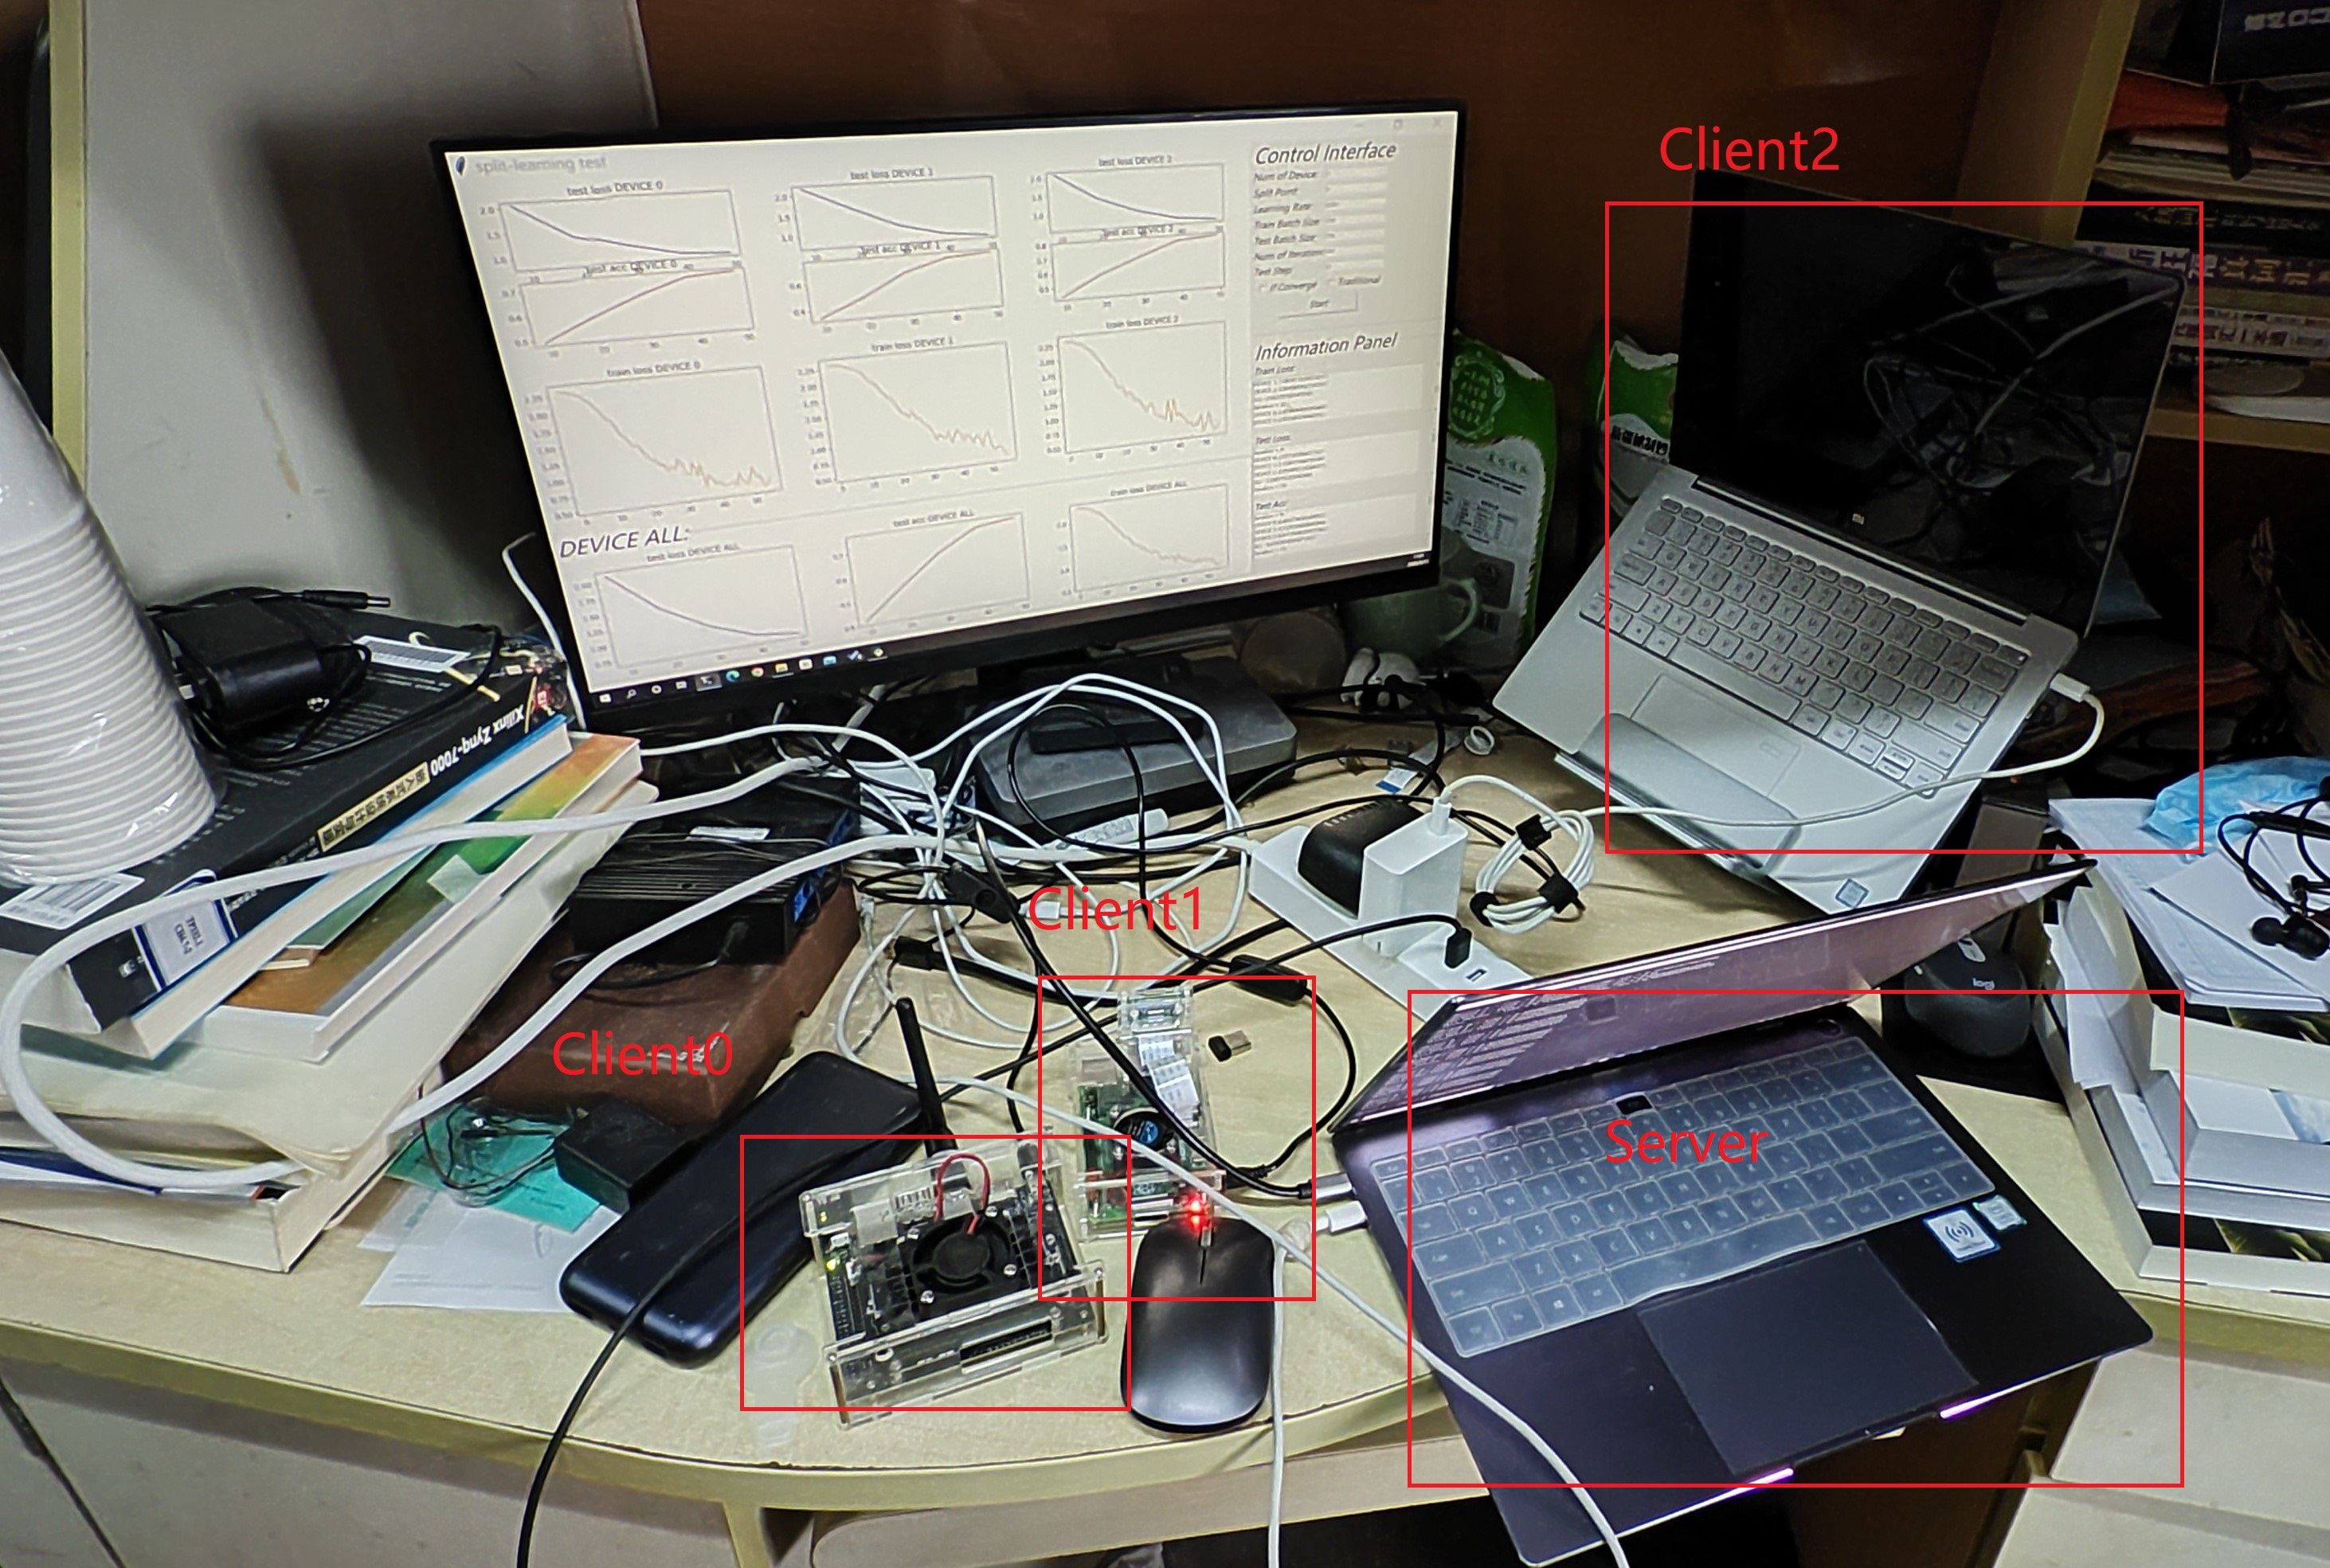
\includegraphics[width=0.85\textwidth]{./figure/5.jpg}  
    \caption*{图10.实物测试}
\end{figure}

图形界面如下,
\begin{figure}[H]
    \centering
    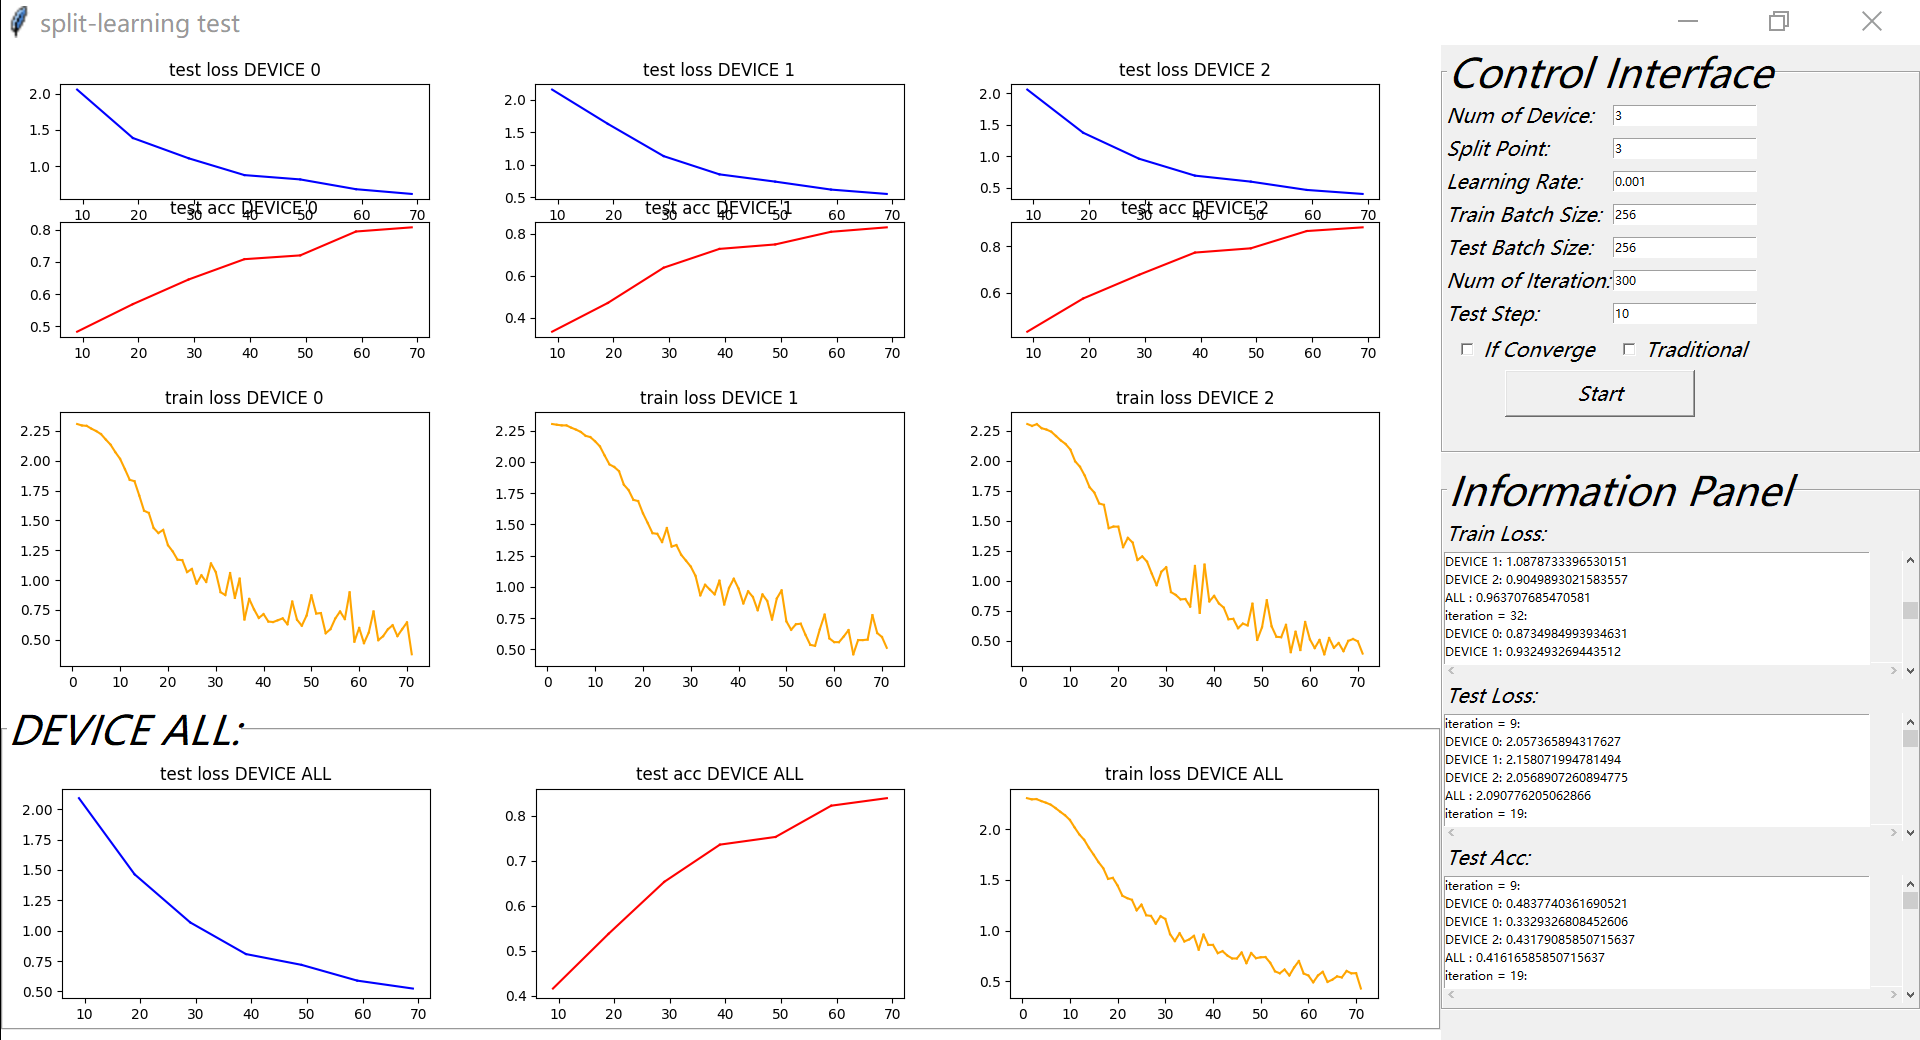
\includegraphics[width=0.85\textwidth]{./figure/6.png}  
    \caption*{图11.服务器端图形界面}
\end{figure}

在右侧的控制台输入用户个数、分割点、学习率、训练和测试的$Batch\_Size$、迭代次数以及测试间隔。与此同时,选择是否共享本地权重,或者是否为传统联邦学习。
按下确定按钮后,这些参数会通过TCP传输到各个用户,即这里的终端设备。然后终端设备和服务器端进行程序化通信,进行分布式学习训练。

每次迭代训练和测试的结果也会传到服务端,显示在图形界面上,除了文字信息外,还会时时绘制图像在左侧主界面上。

\section{参考文献}
% \textit{}
    \textit{[1] Singh, A., Vepakomma, P., Gupta, O., and Raskar, R., “Detailed comparison of communication efficiency of split learning and federated learning”, arXiv e-prints, 2019.}
    
    \textit{[2] Y. Mao, C. You, J. Zhang, K. Huang and K. B. Letaief, "A Survey on Mobile Edge Computing: The Communication Perspective," in IEEE Communications Surveys Tutorials, vol. 19, no. 4, pp. 2322-2358, Fourthquarter 2017, doi: 10.1109/COMST.2017.2745201.}
    
    \textit{[3] Zhu, G., Liu, D., Du, Y., You, C., Zhang, J., and Huang, K., “Towards an Intelligent Edge: Wireless Communication Meets Machine Learning”, arXiv e-prints, 2018.}
    
    \textit{[4] Park, J., Samarakoon, S., Bennis, M., and Debbah, M., “Wireless Network Intelligence at the Edge”, arXiv e-prints, 2018.}
    
    \textit{[5] Li, T., Sahu, A. K., Talwalkar, A., and Smith, V., “Federated Learning: Challenges, Methods, and Future Directions”, IEEE Signal Processing Magazine, vol. 37, no. 3, pp. 50–60, 2020. doi:10.1109/MSP.2020.2975749.}
    
    \textit{[6] Konečný, J., Brendan McMahan, H., Yu, F. X., Richtárik, P., Theertha Suresh, A., and Bacon, D., “Federated Learning: Strategies for Improving Communication Efficiency”, arXiv e-prints, 2016.}
    
    \textit{[7] Yang, K., Jiang, T., Shi, Y., and Ding, Z., “Federated Learning via Over-the-Air Computation”, arXiv e-prints, 2018.}
    
    \textit{[8] Chen, M., Yang, Z., Saad, W., Yin, C., Poor, H. V., and Cui, S., “A Joint Learning and Communications Framework for Federated Learning over Wireless Networks”, arXiv e-prints, 2019.}
    
    \textit{[9] Yang, H. H., Liu, Z., Quek, T. Q. S., and Poor, H. V., “Scheduling Policies for Federated Learning in Wireless Networks”, arXiv eprints, 2019.}
    
    \textit{[10] Ren, J., He, Y., Wen, D., Yu, G., Huang, K., and Guo, D., “Scheduling for Cellular Federated Edge Learning with Importance and Channel Awareness”, arXiv e-prints, 2020.}



\end{document}
